\documentclass[12pt,a4paper,oneside]{book} % twoside for draf

%\usepackage{babel}
\usepackage[utf8]{vietnam}
%\usepackage{times}
%\usepackage{graphicx}

\usepackage{mathptmx}	% same Time New Roma

%\renewcommand{\rmdefault}{phv} % Arial
%\renewcommand{\sfdefault}{phv} % Arial
% \usepackage[fontsize=13pt]{scrextend}

\usepackage[acronym]{glossaries}

\usepackage{fancyhdr}
% \usepackage[utf8]{inputenc}
\usepackage[vietnamese]{babel}
\usepackage{titlesec}
\usepackage{titletoc}
\usepackage{listings}
\usepackage[bookmarks=true]{hyperref}
\usepackage[left=3cm,right=2cm,top=2.5cm,bottom=3cm]{geometry}
\usepackage{graphicx}
\usepackage{hyperref}
\usepackage{tikz}
\usepackage{varwidth}
\usepackage{float}
\usepackage{color}
\usepackage{multirow}
\usepackage{booktabs}
\usepackage[linesnumbered,lined,ruled,resetcount, algochapter]{algorithm2e}
\usepackage{svg}
\usepackage{tabularx}
\usepackage{nomencl}
\usepackage{scrfontsizes}
\usepackage{longtable}
\usepackage{multicol}
\usepackage[toc,page]{appendix}
\usepackage{adjustbox}

\usepackage{makecell}
\usepackage{longtable}
\usepackage{multirow}
% \usepackage{algpseudocode}
\usepackage{setting/bkthesis}
\usepackage[toc]{appendix}

\usepackage{amsmath}

\newtheorem{definition}{Định nghĩa}

\newcommand\sbullet[1][.5]{\mathbin{\vcenter{\hbox{\scalebox{#1}{$\bullet$}}}}}

%\counterwithin{figure}{chapter}
\usepackage[
backend=biber,
bibstyle=authoryear,
sorting=none,
citestyle=numeric-comp
]{biblatex}
\usepackage{xpatch}

\makeatletter
\input{numeric.bbx}
\makeatother

\xpatchbibmacro{date+extrayear}{%
  \printtext[parens]%
}{%
  \setunit{\addperiod\space}%
  \printtext%
}{}{}


\addbibresource{refs.bib}      

% \renewcommand\labelitemi{--}

\setlength{\parskip}{6pt}

\usetikzlibrary{calc}
\setlength{\parindent}{10mm}
\renewcommand{\baselinestretch}{1.3}
\graphicspath{{images/}}
\renewcommand{\listalgorithmcfname}{Danh sách thuật toán}
\renewcommand{\nomname}{Danh sách ký hiệu, viết tắt}
\renewcommand\appendixtocname{Phụ lục}

\SetKwRepeat{Do}{do}{while}%

% \algdef{SE}[DOWHILE]{Do}{doWhile}{\algorithmicdo}[1]{\algorithmicwhile\ #1}%
% \usepackage{setting/uetthesis}

%%% The following lines add Chapter or Appendix in front of the number
\titlecontents{chapter}%
[0pt]%
{\vspace{1ex}}%
{\bfseries Chương \thecontentslabel\quad}%
{\bfseries}%
{\bfseries\hfill\contentspage}
%%% Initially, for the main part of the document, set the label to "Chapter"
\let\chapappname\chaptername

% \thesislayout
% hyper setup
\definecolor{dkgreen}{rgb}{0,0.6,0}
\definecolor{gray}{rgb}{0.5,0.5,0.5}
\definecolor{mauve}{rgb}{0.58,0,0.82}

% setup code area as listings
\lstset{frame=tb,
  language=Java,
  xleftmargin=10pt,xrightmargin=10pt,
%   framesep=2cm,
%   aboveskip=2cm,
%   belowskip=2cm,
  showstringspaces=false,
  columns=flexible,
  basicstyle={\small\ttfamily},
  numbers=left,
  numberstyle=\tiny\color{gray},
  keywordstyle=\color{blue},
  commentstyle=\color{dkgreen},
  stringstyle=\color{mauve},
  breaklines=true,
  breakatwhitespace=true,
  tabsize=2,
  escapeinside={(*@}{@*)}
}

\hypersetup{
	bookmarks=true,
	pdftitle={Công cụ hỗ trợ kiểm tra sự tuân thủ các quy chuẩn viết mã nguồn Java},
	pdfauthor={Nguyễn Việt Hòa}, % author
	pdfsubject={TeX and LaTeX},
	pdfkeywords={TeX, LaTeX, graphics, images}, % list of keywords
	colorlinks=false,       % false: boxed links; true: colored links
	linkcolor=black,       % color of internal links
	citecolor=black,       % color of links to bibliography
	filecolor=black,        % color of file links
	urlcolor=black,        % color of external links
	linktoc=page            % only page is linked
}

\lstdefinelanguage{JavaScript}{
  morekeywords=[1]{break, continue, delete, else, for, function, if, in,
    new, return, this, typeof, var, void, while, with},
  % Literals, primitive types, and reference types.
  morekeywords=[2]{false, null, true, boolean, number, undefined,
    Array, Boolean, Date, Math, Number, String, Object},
  % Built-ins.
  morekeywords=[3]{eval, parseInt, parseFloat, escape, unescape},
  sensitive,
  morecomment=[s]{/*}{*/},
  morecomment=[l]//,
  morecomment=[s]{/**}{*/}, % JavaDoc style comments
  morestring=[b]',
  morestring=[b]"
}[keywords, comments, strings]  
\lstalias[]{ES6}[ECMAScript2015]{JavaScript}

\renewcommand{\lstlistingname}{Mã nguồn}
\renewcommand\thechapter{\arabic{chapter}}
\renewcommand\thesection{\thechapter.\arabic{section}.}
\renewcommand\thesubsection{\thesection\arabic{subsection}.}
\renewcommand{\thetable}{\thechapter.\arabic{table}}
\renewcommand{\thefigure}{\thechapter.\arabic{figure}}
\renewcommand{\thealgocf}{\thechapter.\arabic{algocf}}


\newglossaryentry{latex}
{
    name=latex,
    description={Is a markup language specially suited 
    for scientific documents}
}



\newglossaryentry{OSA}
{
    name=OSA,
    description={Obstructive Sleep Apnea - Hội chứng ngưng thở khi ngủ do tắc nghẽn}
}

\newglossaryentry{AHI}
{
    name=AHI,
    description={Apnea-Hypopnea Index - Chỉ số ngưng thở giảm thở }
}

\newglossaryentry{PSG}
{
    name=PSG,
    description={Polysomnography - Đa ký giấc ngủ }
}

\newglossaryentry{BLE}
{
    name=BLE,
    description={Bluetooth Low Energy - Bluetooth năng lượng thấp }
}

\newglossaryentry{GATT}
{
    name=GATT,
    description={Generic ATTribute Profile- Đặc điểm cấu hình chung }
}




\makeglossaries



\begin{document}
\renewcommand{\thelstlisting}{\thechapter.\arabic{lstlisting}}

\renewcommand{\thedefinition}{\thechapter.\arabic{definition}}



% \makeatletter 
% \renewcommand\thealgorithm{\thechapter.\arabic{algorithm}} 
% \makeatother

\pagestyle{plain}
\frontmatter


%-------TITLE PAGE------%
\begin{titlepage}
	\center
	\begin{tikzpicture}[overlay,remember picture]
		\draw [line width=3pt,rounded corners=0pt,]
		($ (current page.north west) + (25mm,-25mm) $)
		rectangle
		($ (current page.south east) + (-15mm,25mm) $);
		\draw [line width=1pt,rounded corners=0pt]
		($ (current page.north west) + (26.5mm,-26.5mm) $)
		rectangle
		($ (current page.south east) + (-16.5mm,26.5mm) $);
	\end{tikzpicture}
	
	{\large \bfseries ĐẠI HỌC QUỐC GIA HÀ NỘI\\ TRƯỜNG ĐẠI HỌC CÔNG NGHỆ}\\[1cm]
	
\includegraphics[width=0.25\linewidth]{images/Logo_UET.png}\\[1cm]
	{\Large  \bfseries Trần Hữu Nam}\\[1cm]
% 	{ \LARGE \bfseries  XÂY DỰNG CÔNG CỤ KIỂM THỬ TỰ ĐỘNG }\\[0.05cm]
%     {\LARGE \bfseries CHO CÁC ỨNG DỤNG SỬ DỤNG NGÔN NGỮ}\\[0.2cm]
%      { \LARGE \bfseries   TYPESCRIPT}\\[0.5cm]
% 	\hfill\\[2cm]
	{ \LARGE \bfseries  
        NGHIÊN CỨU, PHÁT TRIỂN THIẾT BỊ XÁC ĐỊNH TƯ THẾ NGỦ SỬ DỤNG CẢM BIẾN GIA TỐC}\\[0.05cm]
	\hfill\\[1cm]
	{\large \bfseries LUẬN VĂN THẠC SĨ}\\	
	% {\large \bfseries Ngành: Kĩ thuật điện tử}	
	\hfill\\[5.3cm]	
	{\large \bfseries HÀ NỘI - 2025}\\	
	\vfill
\end{titlepage}

%-------TITLE PAGE+6hbk,------%
\begin{titlepage}
	\center
	\begin{tikzpicture}[overlay,remember picture]
	\draw [line width=3pt,rounded corners=0pt,]
	($ (current page.north west) + (25mm,-25mm) $)
	rectangle
	($ (current page.south east) + (-15mm,25mm) $);
	\draw [line width=1pt,rounded corners=0pt]
	($ (current page.north west) + (26.5mm,-26.5mm) $)
	rectangle
	($ (current page.south east) + (-16.5mm,26.5mm) $);
	\end{tikzpicture}
	
	{\large \bfseries ĐẠI HỌC QUỐC GIA HÀ NỘI\\ TRƯỜNG ĐẠI HỌC CÔNG NGHỆ}\\[2cm]
% 	
\includegraphics[width=0.25\linewidth]{images/Logo_UET.png}\\[1cm]
	
	{\Large  \bfseries Trần Hữu Nam}\\[2cm]		
	{ \LARGE \bfseries  NGHIÊN CỨU, PHÁT TRIỂN THIẾT BỊ XÁC ĐỊNH TƯ THẾ NGỦ SỬ DỤNG
                       CẢM BIẾN GIA TỐC
    }\\[0.05cm]
	\hfill\\[1cm]
	\begin{flushleft}
	{\large \bfseries Ngành: Điện tử viễn thông}\\
	{\large \bfseries Chuyên ngành: Kĩ thuật điện tử}\\
	{\large \bfseries Mã số: 23025029}\\
    
	\end{flushleft}
	\hfill\\[1cm]	
	{\large \bfseries LUẬN VĂN THẠC SĨ}\\
	\hfill\\[1cm]
    
	{\large \bfseries NGƯỜI HƯỚNG DẪN KHOA HỌC: PGS.TS. Mai Anh Tuấn}\\	
    
    
	\begin{flushleft}
% 	{\large \bfseries Cán bộ đồng hướng dẫn: CN. Bùi Quang Cường}\\	
	\end{flushleft}
		\hfill\\[3cm]	
	{\large \bfseries HÀ NỘI - 2025}\\		
	\vfill		
\end{titlepage}

\changefontsizes[16pt]{14pt}
\addtocontents{toc}{\vspace{-1cm}}
\addcontentsline{toc}{chapter}{Lời cam đoan}
\begin{center}
    \textbf{LỜI CAM ĐOAN}
\end{center}
Tôi xin cam đoan: đề tài luận văn thạc sĩ “Nghiên cứu, phát triển thiết bị xác định tư thế ngủ sử dụng cảm biến gia tốc” là công trình nghiên cứu của tôi dưới sự hướng dẫn của thầy \textbf{PGS. TS. Mai Anh Tuấn} và thầy \textbf{ThS. Trần Ngọc Thái} cùng với sự tham khảo từ những tài liệu đã liệt kê trong mục Tài liệu tham khảo. Tôi không sao chép công trình nghiên cứu của cá nhân khác dưới bất kỳ hình thức nào. Nếu có tôi xin hoàn toàn chịu trách nhiệm.

\begin{flushright}
	\begin{varwidth}{\linewidth}\centering
		Hà Nội, ngày \space\space\space\space tháng  \space\space\space\space năm 2025\\
		Học viên\\[2cm]
		Trần Hữu Nam
	\end{varwidth}
\end{flushright}

\newpage

\addcontentsline{toc}{chapter}{Lời cảm ơn}
\begin{center}
    \textbf{LỜI CẢM ƠN}
\end{center}

Lời đầu tiên, tôi xin gửi lời cảm ơn đến thầy PGS.TS. Mai Anh Tuấn và thầy ThS. Trần Ngọc Thái vì đã tận tình hướng dẫn, truyền đạt kiến thức cho tôi trong suốt quá trình học tập và thực hiện đề tài. 
Tôi xin cảm ơn tập thể thầy, cô khoa “Điện tử Viễn thông”,  Trường Đại học Công nghệ - ĐHQGHN, đã giảng dạy tôi trong quá trình tôi học tập tại trường. Tôi cũng xin cảm ơn các anh chị ở Bộ môn Công nghệ Vi cơ Điện tử và Kỹ thuật Máy tính đã tạo điều kiện giúp đỡ, chỉ bảo tôi trong thời gian làm khóa luận. 
Cuối cùng, tôi xin cảm ơn bố mẹ, gia đình cũng như bạn bè, tập thể lớp K30 đã luôn đồng hành, chia sẻ và động viên tôi suốt thời gian qua.


\newpage
\addcontentsline{toc}{chapter}{Tóm tắt}
\begin{center}
    \textbf{TÓM TẮT}
\end{center}
% \changefontsizes[16pt]{12pt}
\textit{\textbf{Tóm tắt: }} 
Ngưng thở tắc nghẽn khi ngủ (Obstructive Sleep Apnea - OSA) là tình trạng rối loạn hô hấp khi ngủ thường gặp, được đặc trưng bởi những cơn ngưng/giảm thở ngắn, lặp lại trong khi ngủ, gây gián đoạn giấc ngủ bởi hành vi thức giấc thường xuyên và giảm oxy máu ngắt quãng\cite{Epstein2009}. Nghiên cứu\cite{Salari2025} đã phân tích dữ liệu từ 15 nghiên cứu với tổng cộng 42.924 người. Kết quả cho thấy tỷ lệ mắc chứng buồn ngủ ban ngày quá mức (EDS) ở bệnh nhân ngưng thở tắc nghẽn khi ngủ (OSA) trên toàn cầu là 39,9\% (khoảng tin cậy 95\%: 34,4\%–45,7\%).

Trong bối cảnh công nghệ chế tạo ngày càng phát triển mạnh mẽ, việc thu nhỏ hóa và tối ưu hiệu suất hoạt động của các loại cảm biến, pin đã trở thành một yếu tố then chốt, mang tính quyết định trong quá trình tích hợp chúng vào các thiết bị điện tử có kích thước nhỏ gọn. Không chỉ góp phần nâng cao độ chính xác trong việc đo lường các thông số sinh lý quan trọng, nó còn giúp giảm thiểu kích thước thiết bị, tăng tính di động và mở rộng khả năng ứng dụng trong nhiều lĩnh vực, đặc biệt nổi bật trong y học cá thể hóa.

Bên cạnh đó, sự phát triển vượt bậc của trí tuệ nhân tạo (AI) đóng vai trò như một đòn bẩy quan trọng trong việc nâng cao hiệu quả khai thác dữ liệu cảm biến. AI không chỉ tối ưu hóa quy trình xử lý và phân tích dữ liệu mà còn thúc đẩy khả năng nhận diện mẫu, phân cụm, dự đoán và đưa ra quyết định mang tính hỗ trợ lâm sàng. Trong lĩnh vực chẩn đoán hội chứng ngưng thở khi ngủ, sự phối hợp giữa cảm biến và thuật toán học máy không chỉ đảm bảo độ chính xác cao trong thu thập dữ liệu mà còn mở ra khả năng phân tích chuyên sâu về các yếu tố sinh lý, phục vụ quá trình đánh giá y tế toàn diện.

Trên cơ sở đó, nghiên cứu này tập trung phát triển một thiết bị theo dõi tình trạng bệnh nhân trong khi ngủ, sử dụng cảm biến gia tốc kết hợp với thuật toán học máy nhằm phân tích tư thế ngủ và phát hiện các dấu hiệu liên quan đến hội chứng ngưng thở khi ngủ. Hệ thống được tiến hành nghiên cứu, triển khai trên ứng dụng di động trước rồi được tích hợp trên chip, hướng đến khả năng giám sát liên tục, thu thập dữ liệu thời gian thực và đưa ra đánh giá có độ tin cậy cao, góp phần cải thiện hiệu quả trong phát hiện sớm và hỗ trợ điều trị bệnh lý hô hấp liên quan đến giấc ngủ.


\vspace{-0.5cm}
\begin{flushleft}
  \textit{\textbf{Từ khóa: } cảm biến gia tốc, học máy, ngưng thở khi ngủ}
\end{flushleft}
% \changefontsizes[16pt]{13pt}



\changefontsizes[16pt]{13pt}


% \changefontsizes[16pt]{14pt}
% \input{chapters/0.2.start}

\tableofcontents

% \pagestyle{fancy}

\addcontentsline{toc}{chapter}{\listfigurename}
\listoffigures


\listoftables
\addcontentsline{toc}{chapter}{\listtablename}

\printglossaries

% \newpage
% \chapter*{Thuật ngữ}

% \addcontentsline{toc}{chapter}{Thuật ngữ}
% \begin{table}[h!]
%     \centering
%     \begin{adjustbox}{width=1\textwidth}
%     \small
%     \begin{tabular}{|c|c|c|}
%          \hline
%          \textbf{Từ viết tắt} & \textbf{Từ đầy đủ} &\textbf{Ý nghĩa}\\
%          \hline
%         API   & Application Programming Interface & Giao diện lập trình ứng dụng\\
%         \hline
%         AST   & Abstract Syntax Tree & Cây cú pháp trừu tượng\\
%         \hline
%          BDD   & Behaviour Driven Development & Mô hình phát triển phần mềm định hướng hành vi\\
%         \hline
%         CFG   & Control Flow Graph & Đồ thị dòng điều khiển\\
%          \hline
%         CFT   & Control Flow Testing & Kiểm thử dòng điều khiển\\
%          \hline
%         DFT  & Data Flow Testing & Kiểm thử dòng dữ liệu\\
%         \hline
%         HTML   & Hyper Text Markup Language & Ngôn ngữ đánh dấu siêu văn bản\\
%         \hline
%         JSON   & JavaScript Object Notation & Cú pháp lưu trữ và trao đổi dữ liệu\\
%         \hline
%         MC/DC   & Modified Condition/Decision Coverage & Bao phủ quyết định sửa đổi\\
%         \hline
%         OOP   & Object-oriented Programming & Lập trình hướng đối tượng\\
%          \hline
%         SE   & Symbolic Execution & Thực thi tượng trưng\\
%         \hline
%         SMT   & Satisfiability Modulo Theories & Lý thuyết mô-đun thỏa mãn\\
%         \hline
%         TDD   & Test Driven Development & Mô hình phát triển phần mềm định hướng kiểm thử\\
%         \hline
%         XML   & Extensible Markup Language & Ngôn ngữ đánh dấu có thể mở rộng\\
%         \hline
%         \end{tabular}
%     \end{adjustbox}
%     % \caption{Bảng thuật ngữ được sử dụng trong khóa luận}
%     \label{table:1}
% \end{table}

\mainmatter



\changefontsizes[16pt]{13pt}
\chapter*{Đặt vấn đề}
\addcontentsline{toc}{chapter}{Đặt vấn đề}
\thispagestyle{empty}
Ngưng thở tắc nghẽn khi ngủ (Obstructive Sleep Apnoea – OSA) là một rối loạn hô hấp phổ biến trong giấc ngủ, được đặc trưng bởi các đợt ngưng thở hoặc giảm thông khí tắc nghẽn lặp đi lặp lại trong lúc ngủ, dẫn đến việc gián đoạn giấc ngủ do vi thức giấc và giảm oxy trong máu.  Tỷ lệ hiện mắc OSA tại Việt Nam ước tính khoảng 8,5\% \cite{nguoimacOSA_VN}. OSA hiện được công nhận là một yếu tố có nguy cơ độc lập đối với nhiều bệnh lý liên quan đến tim mạch, đặc biệt là tăng huyết áp. Ngoài ra, hội chứng này còn có mối liên hệ đáng kể với các nguy cơ như tai nạn giao thông, tai nạn lao động dẫn đến làm gia tăng gánh nặng kinh tế xã hội\cite{osa_bike}\cite{Marin2005}\cite{drive_osa}. Đáng chú ý, tình trạng ngưng thở khi ngủ kéo dài và không được phát hiện, điều trị có thể ảnh hưởng nghiêm trọng đến sức khỏe gây ra rối loạn nhịp tim và một trong những nguyên nhân gây đột tử \cite{sumarry_osa}. Theo PSG.TS Nguyễn Thy Khuê, Hội Y học Giấc ngủ Việt Nam, ngưng thở khi ngủ còn là một trong nhưng dấu hiệu rõ ràng của bệnh đái tháo đường, bệnh thận \cite{bsThyKhue}. OSA được phát hiện ở hơn 20\% người bệnh đái tháo đường và làm trầm trọng thêm các rối loạn chuyển hóa, đặc biệt là đái tháo đường type 2. Trong một nghiên cứu tiêu biểu tại Việt Nam, GS.TS. Dương Quý Sỹ và cộng sự đã khảo sát 524 trẻ em mắc rối loạn tăng động giảm chú ý (Attention Deficit Hyperactivity Disorder - ADHD) tại Bệnh viện Nhi Trung ương Việt Nam. Kết quả cho thấy tỷ lệ mắc (OSA) ở nhóm này là 23.3\%, trong đó chủ yếu ở mức độ trung bình đến nặng \cite{ThaySUCHildren}. Nghiên cứu cũng đồng thời xác định mối tương quan đáng kể giữa mức độ nghiêm trọng của OSA và các triệu chứng mất tập trung, tăng động, rối loạn hành vi, lo âu và trầm cảm. Phát hiện nhấn mạnh sự cần thiết của việc sàng lọc OSA trong quá trình điều trị toàn diện ADHD ở trẻ em. 

Một dạng đặc biệt của OSA được ghi nhận là ngưng thở khi ngủ do tư thế (Positional Obstructive Sleep Apnea - pOSA). Bệnh nhân được chẩn đoán mắc pOSA có chỉ số AHI lớn hơn 5, và giá trị AHI ở tư thế ngửa cao gấp ít nhất hai lần so với nằm ở tư thế khác \cite{heinzer2018}. Các nghiên cứu gần đây chỉ ra rằng tỷ lệ mắc pOSA lên tới 50\% bệnh nhân OSA \cite{sabil2020}. Điều này cho thấy tư thế ngủ có ảnh hưởng sinh lý rõ rệt đến sự sụp đổ đường thở trên, đặc biệt ở tư thế nằm ngữa. Lúc nằm ngửa, trọng lực làm xẹp các cơ vùng họng dẫn đến làm hẹp khoang khí.

Việc chẩn đoán hội chứng ngưng thở tắc nghẽn khi ngủ (OSA) hiện nay chủ yếu được thực hiện thông qua hai phương pháp: đa ký giấc ngủ (Polysomnography – PSG) và thiết bị kiểm tra giấc ngủ tại nhà (Home Sleep Test – HST). Trong đó, PSG được xem là tiêu chuẩn vàng trong việc đánh giá OSA. DO phương pháp này cho phép thu thập đồng thời nhiều thông số sinh lý quan trọng bao gồm: luồng khí hô hấp qua mũi và/hoặc miệng, cử động thành ngực và bụng, tiếng ngáy, điện não đồ (Electroencephalography – EEG), điện tâm đồ (Electrocardiography – ECG), điện cơ đồ (Electromyography – EMG), và độ bão hòa oxy trong máu (SpO$_2$). Quá trình do PSG phải được thực hiện trong môi trường có kiểm soát tại các cơ sở y tế chuyên khoa, dưới sự giám sát trực tiếp của bác sỹ chuyên ngành giấc ngủ hoặc kĩ thuật viên có chuyên môn\cite{psg_paper}\cite{kushida2005psg}. 

Mặc dù PSG vẫn giữ vai trò là phương pháp tham chiếu trong chẩn đoán và theo dõi chất lượng giấc ngủ cũng như các rối loạn liên quan, nhưng việc triển khai kỹ thuật này thường đòi hỏi chi phí cao, trang thiết bị chuyên dụng và điều kiện thực hiện tại các cơ sở y tế chuyên khoa. Một thách thức khác của PSG là người bệnh thường cảm thấy bất tiện và cảm giác khó chịu do mang nhiều cảm biến gắn trên cơ thể trong suốt đêm, dẫn đến nguy cơ gián đoạn hoặc sai lệnh dữ liệu trong quá trình ghi nhận. Vì vậy, các hệ thống HST đang ngày càng thu hút sự quan tâm từ cộng đồng khoa học toàn cầu\cite{e3hst}\cite{hstSurvey}\cite{hst_paper}. Các thiết bị HST hiện đại dùng các cảm biến không xâm lấn nhằm ghi nhận và phân tích một số tín hiệu sinh lý cơ bản như luồng khí hô hấp, tư thế ngủ, áp suất mũi, độ bão hòa oxy và nhịp tim. Việc cải thiện chất lượng, kéo dài thời lượng sử dụng và tăng độ chính xác và cải thiện mức độ thoải mái vẫn là những thách thức lớn đối với giới nghiên cứu và các nhà sản xuất thiết bị y tế. Tuy nhiên, với những tiến bộ công nghệ đang diễn ra nhanh chóng, HST có tiềm năng trở thành một công cụ chẩn đoán quan trọng và được ứng dụng rộng rãi trong lâm sàng. Điều này không chỉ mang lại sự thuận tiện và chấp nhận cao hơn từ phía người bệnh, mà còn góp phần làm giảm gánh nặng chi phí và áp lực cho hệ thống chăm sóc sức khỏe.

Trong những năm gần đây, nhiều nhóm nghiên đang chú trọng nghiên cứu, phát triển hệ thống HST nhằm mục đích thay thế hoặc hỗ trợ cho đa ký giấc ngủ. Năm 2011, Collop và cộng sự đã phát triển một hệ thống phân loại SCOPER (Sleep, Cardiovacular, Oximetry, Position, Effort, and Respiration) để đánh giá các tín hiệu sinh lý thu nhận trong việc chẩn đoán OSA\cite{hst_6p_paper}. Tác giả Morillo D và cộng sự đề xuất một phương pháp sàng lọc ngưng thở tắc nghẽn khi ngủ dựa trên cảm biến gia tốc gắn tại vị trí hõm ức, cho phép trích xuất các tín hiệu hô hấp, tim mạch và tiếng ngáy bằng kỹ thuật xử lý tín hiệu số, từ đó chứng minh tính khả thi của thiết bị di động đơn giản và chi phí thấp trong hỗ trợ chẩn đoán hội chứng ngưng thở – giảm thở khi ngủ\cite{morillo2010accelerometer}. Trong nhóm các thiết bị đeo, A.H. Yüzer và cộng sự đã phát triển thiết bị đeo tay sử dụng cảm biến gia tốc ADXL345 để phát hiện và phát tín hiệu rung khi cảnh báo. \cite{hst_wear_paper}. Tương tự, nhóm Yunyoung Nam và cộng sự cũng đã tích hợp hệ thống thu thập, phân tích sử dụng một cảm biến gia tốc ba trục và một cảm biến áp suất để giám sát chất lượng giấc ngủ tư thế ngủ, trạng thái ngủ, giai đoạn ngủ (REM và chu kỳ giai đoạn ngủ không REM) \cite{hst_pressure_paper}. Tại Việt Nam, nhóm nghiên cứu của  Giáo sư Lê Tiến Thường, trường đại học Bách Khoa TP Hồ Chí Minh đã sử dụng cảm biến gia tốc MPU6050 cùng với vi xử lý ESP32 nhằm ghi nhận hơi thở và nhịp tim của bệnh nhân OSA thông qua rung động, và dòng chảy của động mạch và tĩnh mạch ở cổ \cite{thuong_wear_paper}. Gần đây, Domingues và cộng sự (2024) xây dựng một mô hình mạng nơ-ron nhân tạo dựa trên dữ liệu từ máy đo SPO2, cấm biến gia tốc và ghi âm tiếng ngáy của hệ thống Biologix, nhằm dự đoán chính xác trạng thái ngủ. Kết quả cho thấy mô hình này có khả nâng cao độ chính xác trong chẩn đoán ngưng thở khi ngủ tại nhà, tiệm cận với tiêu chuẩn của đa ký giấc ngủ truyền thống \cite{domingues2024sleep}. Một hướng nghiên cứu khác là cảm biến đặt dưới nệm giường. Tác giả Andrei Boiko và cộng sự đánh giá hệ thống phát sử dụng cảm biến gia tốc đặt dưới đệm giường để ghi dao động do cử động ngực khi thở. Kết quả cho thấy thuật toán phát hiện ngưng thở đạt độ chính xác, độ đặc hiệu và độ nhạy lần lượt là 94.6\%, 95.3\% và 93.7\% \cite{Boiko2023}. 

Nhìn chung, việc chẩn đoán OSA hay pOSA đòi hỏi hệ thống cần có khả năng thu thập liên tục, và đưa ra quyết định chính xác dựa trên những dữ liệu đó. Do đó, việc xây dựng các mô hình học máy để phân loại AHI, hay các tư thế ngủ đang là 1 hướng nghiên cứu phổ biến hợp hợp cả hai lĩnh vực y tế giấc ngủ và công nghệ dữ liệu. Các nghiên cứu tiêu biểu sử dụng mô hình như Decision Tree, Ramdom Forest, SVM và các mô hình Deep Learning cho độ chính xác từ 



Khóa luận văn có mục đích nghiên cứu, ứng dụng cảm biến gia tốc kết hợp với các bộ lọc tín hiệu, trí tuệ nhân tạo, ứng dụng phần mềm để tạo ra một sản phẩm có độ chính xác, tính ứng dụng cao trong cuộc sống. Khóa luận đưa ra cái nhìn tổng quan về chứng ngưng thở khi ngủ và thiết bị chẩn đoán sử dụng cảm biến gia tốc. Kết quả có tiềm năng ứng dụng thực tế phục vụ cho mục đích chuẩn đoán, đánh giá và phân tích về chứng ngưng thở khi ngủ. Khóa luận này trình bày thiết kế, chế tạo và thử nghiệm một thiết bị đeo được tích hợp cảm biến gia tốc 3 trục cho phép tiến hành thực nghiệm chế tạo và thiết lập hệ thống đo đạc cho cảm biến đã đề xuất với những mục tiêu cụ thể: 01) Tăng độ chính xác của hệ thống, 02) Thu nhỏ thiết kế mạch, 03) Tăng trường khả năng lưu trữ dữ liệu và 04) Hỗ trợ người sử dụng thông qua phần mềm ứng dụng. Khóa luận được thực hiện thông qua 01) tham khảo tài liệu, 02) Phương pháp nghiên cứu lý thuyết, 03) phương pháp thực nghiệm. Nội dung nghiên cứu được trình bày trong 3 chương như sau:

    Chương 1: Tổng quan về OSA và các thiết bị theo dõi.

    Chương 2: Quá trình lựa chọn và xây dựng thiết bị.

    Chương 3: Kết quả thực nghiệm, đánh giá và kế hoạch nghiên cứu trong thời gian tới.


\chapter{Tổng quan về OSA và các thiết bị theo dõi \label{background_section}}

\section{Giới thiệu về chứng ngưng thở trong lúc ngủ}
\gls{OSA}\cite{osa_summary}\cite{ThaySYOSA} là tình trạng xảy ra khi đường hô hấp trên bị tắc nghẽn một phần hoặc hoàn toàn trong ít nhất 10 giây, mặc dù cơ thể vẫn nỗ lực hô hấp thông qua chuyển động của ngực và bụng. Các triệu chứng thường gặp của OSA bao gồm buồn ngủ quá mức vào ban ngày, mệt mỏi, ngáy to, thức giấc ngắn lặp đi lặp lại (vi thức tỉnh), và đau đầu khi thức dậy vào buổi sáng. OSA làm độ bão hòa oxi trong máu giảm xuống khi đó các cơ sẽ cố gắng để chống lại việc này khiến người bị OSA sẽ có thể thức dậy. Các mức độ của hội chứng ngưng thở khi ngủ do tắc nghẽn (OSA) được đánh giá dựa trên chỉ số ngưng thở giảm thở (Apnea–Hypopnea Index - AHI) bằng cách chia tổng số lần ngưng thở và hẹp thở cho tổng số giờ đã ngủ, với mỗi sự kiện phải kéo dài ít nhất 10 giây \ref{ahi}.

\begin{table}[h!]
\caption{Phân loại mức độ ngưng thở khi ngủ theo chỉ số \gls{AHI}}
\label{ahi}
\vspace{-3mm}
\begin{center}
\begin{tabular}{|c|c|}
\hline
AHI & Cấp độ \\
\hline
<5 & Không mắc \\
5 đến 10 & Nhẹ \\
15 đến 30 & Trung bình \\
>30 & Nặng \\
\hline
\end{tabular}
\label{tab1}
\end{center}
\end{table}


1)Ngưng thở tắc nghẽn (Obstructive Apnea): Là tình trạng ngưng thở gần như hoàn toàn (>90\%) trong thời gian ít nhất 10 giây, mặc dù vẫn có nỗ lực hô hấp từ lồng ngực và bụng. 2)Giảm hô hấp (Hypopnea): Là sự giảm luồng khí hô hấp > 30\%, đi kèm với giảm độ bão hòa oxy trong máu >3\% hoặc gây thức giấc. Tỷ lệ ngưng thở tắc nghẽn là từ 2\% đến 9\% ở người lớn. Ngưng thở tắc nghẽn khi ngủ có thể tăng gấp 4 lần ở nam giới và gấp 7 lần hơn ở những người béo phì (ví dụ chỉ số khối cơ thể (Body mass Index - BMI) > 30). OSA nặng (AHI > 30/h) làm tăng nguy cơ tử vong ở nam giới trung niên.

Ngưng thở khi ngủ do tắc nghẽn thường xảy ra ở người lớn tuổi và những người thừa cân béo phì. Yếu tố gây ra có thể liên quan đến cấu trúc hoặc phi cấu trúc, bao gồm cả yếu tố di truyền. Nguyên nhân chủ yếu là do diện tích vòng họng hoặc khoang mũi bị thu hẹp như viêm xoang, các khối u, bệnh phì đại tuyến lưỡi, amydal, phì đại tuyến mỡ (đặc biệt ở trẻ em), béo phì hoặc đến từ các bệnh lý: tiểu đường, huyết áp cao, các bệnh tim mạch v.v\cite{wright1997health}. Ngoài ra, có thể đến từ thói quen không lành mạnh của con người như là sử dụng các chất kích thích, hút thuốc, ngáy khi ngủ\cite{reason_osa}\cite{reasonOsa}. Bên cạnh đó, các yếu tố không giải phẫu như hoạt động kém của cơ giãn họng, ngưỡng thức giấc thấp và sự điều hòa hô hấp không ổn định cũng góp phần quan trọng vào cơ chế bệnh sinh. Sự tương tác giữa các yếu tố này tạo nên tính đa dạng trong biểu hiện và mức độ nặng của OSA.



Phần lớn bệnh nhân mắc hội chứng ngưng thở khi ngủ tắc nghẽn (\gls{OSA}) không tự nhận thức được các rối loạn hô hấp xảy ra trong lúc ngủ. Điều này đặc biệt đúng với những người sống hoặc ngủ một mình, do thiếu sự quan sát từ bên ngoài. Đặc biệt OSA xuất hiện lớn hơn 80\% ở các bệnh liên quan đến béo phì: tiểu đường, thận, mỡ máu v.v\cite{wright1997health}. Hội chứng ngưng thở khi ngủ tắc nghẽn (OSA) ảnh hưởng nghiêm trọng đến chất lượng cuộc sống của người bệnh. Các hoạt động thường ngày trở nên gián đoạn hoặc khó thực hiện hơn. Hậu quả của OSA bao gồm suy giảm trí nhớ, giảm tỉnh táo, dễ cáu gắt, trầm cảm, đau đầu và giảm khả năng tập trung\cite{flemons1997quality}. Những tác động này dẫn đến hiệu suất làm việc giảm, rối loạn các mối quan hệ xã hội và gia tăng nguy cơ tai nạn giao thông. Một nghiên cứu khác cũng bởi Mooe và cộng sự\cite{mooe1996sleep} ở nam giới cho thấy 37\% bệnh nhân bệnh mạch vành (Coronary Artery Disease - CAD) có AHI > 10. Young và cộng sự (1997) phát hiện rằng chỉ số AHI tăng tỉ lệ thuận với huyết áp tâm thu và tâm trương (p=0.003 và p=0.01)\cite{young1997population}.

Trong điều kiện hiện tại, đa số bệnh nhân nghi ngờ có hội chứng tắc nghẽn ngưng thở khi ngủ được khám bới bs chuyên khoa Tai Mũi Họng và bác sĩ chuyên gia về ngủ ngáy. Khám tổng quát hỏi bệnh sử liên quan với thang điểm ngủ ngáy (ví dụ: Epworth Sleepiness Scale, STOP BANG đã được dịch sang tiếng Việt và được chấp thuận tại Việt Nam như một phương án sáng lọc bệnh nhân OSA) và khám nội soi Tai Mũi Họng để tìm nguyên nhân. Vì đa số các trường hợp ngáy, ngưng thở khi ngủ là do tắc nghẽn ngoại biên, nguyên nhân từ Mũi – Họng – Màn hầu , VA và amidan, và những bất thường về hàm mặt khác. Việc đánh giá ngưng thở lúc ngủ bắt đầu bằng đánh giá giấc ngủ toàn diện, bao gồm khai thác bệnh sử về các triệu chứng hoặc dấu chứng ban đầu sau đó là đánh giá tổng thể qua PSG\cite{diagnosis_osa}\cite{medical2006polysomnography}.
Phương pháp do dùng đa ký giấc ngủ (Polysomnography) với sự giám sát của các bác sĩ chuyên môn được coi là tiêu chuẩn vàng trong chẩn đoán chứng ngưng thở khi ngủ. Polysomnography là một phương pháp ghi đa kênh liên tục trong suốt một đêm, bao gồm nhiều thông số sinh lý nhằm đánh giá toàn diện hoạt động hô hấp và thần kinh khi ngủ. Các thành phần chính trong một xét nghiệm polysomnography bao gồm: điện não đồ (EEG) để ghi lại hoạt động điện của não; điện cơ ký (EMG) nhằm đo trương lực cơ, đặc biệt là ở cằm và chân; điện động mắt (EOG) để theo dõi chuyển động của nhãn cầu, giúp xác định các giai đoạn của giấc ngủ; và điện tâm đồ (ECG) để theo dõi hoạt động điện của tim. Bên cạnh đó, quá trình đo cũng bao gồm theo dõi độ bão hòa oxy trong máu (SpO2), đo lưu lượng khí thở qua mũi và miệng, đánh giá nỗ lực hô hấp thông qua chuyển động của ngực và bụng, đo áp lực khí thở qua mũi, và ghi nhận cường độ tiếng ngáy. Tập hợp các thông số này cho phép bác sĩ chẩn đoán chính xác các rối loạn hô hấp khi ngủ, đặc biệt là hội chứng ngưng thở khi ngủ tắc nghẽn (OSA).

Một trong những hạn chế của phương pháp đánh giá sử dụng (\gls{PSG}) là sự bất tiện, chi phí cao và khả năng phổ biến thấp, nhất là đối với phần lớn người bệnh có thu nhập thấp. Việc yêu cầu bệnh nhân phải lưu trú qua đêm tại cơ sở y tế, cùng với việc gắn nhiều thiết bị theo dõi sinh lý lên cơ thể, không chỉ gây cảm giác khó chịu mà còn tiềm ẩn nguy cơ ảnh hưởng đến chất lượng và tính chính xác của dữ liệu thu thập được. Chính những bất cập này đã thúc đẩy sự phát triển của các thiết bị theo dõi giấc ngủ ngoài trung tâm (Out-of-Center devices) hay còn gọi là thiết bị kiểm tra giấc ngủ tại nhà (Home Sleep Test – HST). Những thiết bị này thường được thiết kế với số lượng cảm biến tối giản hơn so với PSG truyền thống, đồng thời tích hợp các thuật toán phân tích tự động – được xử lý trực tiếp trên thiết bị hoặc thông qua phần mềm chuyên dụng – nhằm hỗ trợ chẩn đoán ngưng thở khi ngủ do tắc nghẽn (OSA) một cách thuận tiện và tiết kiệm hơn. Những thông số SCOPERA được coi là cơ sở để xây dựng thiết bị HST trong đó giấc ngủ (Sleep - S), tim mạch (Cardiovascular - C), oxi trong máu (Oximetry - O), cố gắng thở (Effort - E), luồng không khí lưu thông (Respiratory - R), âm thở (Audio - A). Nghiên cứu\cite{svmHSt2017} chứng minh rằng tín hiệu chuyển động ngực (Thoracic movement signal - THO) và bụng (Abdominal movement signal - ABD), thu từ các dải piezoelectric đeo được, có thể được sử dụng hiệu quả để phân loại các dạng rối loạn thở khi ngủ thông qua mô hình thuật toán SVM. Kết quả cho thấy khi kết hợp cả hai tín hiệu, độ chính xác phân loại đạt trung bình 81.8\%, khẳng định tiềm năng ứng dụng của phương pháp này trong sàng lọc và theo dõi OSA tại nhà hoặc trong lâm sàng.
Theo tìm hiểu của tác giả, thiết bị HST vẫn có cấu hình khá phức tạp với nhiều cảm biến và thao thác cũng chưa hoàn toàn đơn giản, thêm vào đó giá trung bình của thiết bị vào khoảng 2300 USD làm hạn chế khả năng tiếp cận của người sử dụng, đặc biệt là những người có thu nhập trung bình hoặc thấp \cite{hst_review}. Do đó, những nghiên cứu gần đây tập trung theo hướng phát triển thiết bị với ít điện cực hơn để tối giản phần cứng của hệ thống cũng như tích hợp thêm các mô hình học máy hoặc trí tuệ nhân tạo làm tăng tính chính xác và độ lặp lại. Trong luận văn này, tác giả lựa chọn nghiên cứu ban đầu sử dụng cảm biến gia tốc để phát hiện các tư thế ngủ có liên quan tới chứng ngưng thở trong lúc ngủ kết hợp việc xây dựng mô hình học máy hướng tới phát triển một một thiết bị IoT có thể dự đoán mức độ nghiêm trọng của chứng ngưng thở trong lúc ngủ thông qua chỉ số AHI.

\section{Ứng dụng cảm biến gia tốc trong đánh giá tư thế ngủ của người mắc OSA tại nhà}
Đánh giá tư thế ngủ là một thành phần quan trọng trong nghiên cứu giấc ngủ, đặc biệt trong chẩn đoán và theo dõi các rối loạn hô hấp liên quan đến giấc ngủ như hội chứng ngưng thở khi ngủ do tắc nghẽn (OSA). Nhiều phương pháp kỹ thuật đã được phát triển nhằm ghi nhận và phân tích tư thế ngủ một cách chính xác. Các hệ thống ghi hình sử dụng camera hồng ngoại có khả năng thu thập toàn bộ quá trình ngủ trong điều kiện ánh sáng thấp, trong khi đó, các cảm biến gia tốc ba trục (triaxial accelerometers) cho phép nhận diện sự thay đổi tư thế dựa trên dao động và gia tốc của cơ thể. Bên cạnh đó, các thiết bị tích hợp cảm biến áp suất, chẳng hạn như đệm cảm biến, cung cấp thông tin về sự phân bố trọng lực và áp lực tiếp xúc, từ đó suy luận tư thế ngủ một cách gián tiếp nhưng hiệu quả. Những hệ thống tiên tiến hơn còn kết hợp đa cảm biến và tích hợp nhiều phương pháp đồng thời, nhằm nâng cao độ tin cậy, tính định lượng và khả năng ứng dụng trong cả môi trường lâm sàng lẫn tại nhà. Theo S. Akbarian và đồng các tác giả đã đề cập đến phương pháp giám sát tư thế ngủ bằng máy ảnh hồng ngoại kết hợp với công nghệ học sâu (Deep learning) \cite{Akbarian_osa} có kết quả tốt nhưng có khó khăn để xác định các góc các khác nhau của khuôn mặt. Còn theo A. Channa, M. Yousuf và N. Popescu đã sử dụng cảm biến áp suất được gắn dưới đệm để theo dõi thư thế ngủ với 2048 điểm cảm biến \cite{Channa_osa}. Trong đó cảm biến gia tốc 3 trục được đánh giá là phương pháp hiệu quả, tiết kiệm chi phí và độ chính xác cao. Jeng PY và đồng nghiệp đã thực hiện phát triển chế tạo thiết bị đeo tay sử dụng cảm biến gia tốc kết hợp với thiết bị ở ngực để lấy nhãn cho dữ liệu. Các phương pháp học máy truyền thống được sử dụng với độ chính xác đánh giá 4 tư thế khi ngủ trên 85\% \cite{Jeng_osa}. Cách đặt và vị trí đặt cảm biến ảnh hướng rất lớn đến chất lượng, độ chính xác của phép đo. Theo đó vị trí xương ức cổ được xem là vị trí có thể thu được tín hiệu chính xác để đặt đơn cảm biến \cite{Zhang_osa}. Việc sử dụng nhiều cảm biến ở những vị trí khác như cổ tay, trán, … sẽ có thêm nhiều dữ liệu hữu ích để phân tích, đánh giá. Ngoài ra, hiện nay với sự phát triển vượt bậc của điện thoại di động, việc tận dụng cảm biến gia tốc ở ngay trên chính chiếc điện thoại cũng là giải pháp hữu hiệu. Nhóm tác giả trong \cite{Ferrer_osa} đã báo cáo nghiên cứu đánh giá tư thế ngủ của bệnh nhân sử dụng thiết bị di động đeo ở xương ức kết hợp với phần mềm trên nền tảng Android để thu thập lại dữ liệu kể cả khi tắt màn hình. Trong một nghiên cứu tiêu biểu, Natale và cộng sự đã khai thác các cảm biến tích hợp sẵn trên điện thoại iPhone để ước lượng các thông số liên quan đến chất lượng giấc ngủ, bao gồm tổng thời gian ngủ (Total Sleep Time – TST), độ trễ vào giấc (Sleep Onset Latency – SOL) và hiệu quả giấc ngủ (Sleep Efficiency – SE). Phương pháp tiếp cận này cho thấy tiềm năng trong việc sử dụng thiết bị di động như một công cụ theo dõi giấc ngủ tiện lợi và dễ tiếp cận, đặc biệt trong các nghiên cứu cộng đồng và ứng dụng tại nhà\cite{Natale_osa}. Đặc điểm của sử dụng tích hợp cảm biến gia tốc trên điện thoại là rất tiện lợi, sử dụng trực tiếp mà không cần phát triển phần cứng. Tuy nhiên, việc tiếp xúc điện thoại trực tiếp với cơ thể trực tiếp trong thời gian lâu cũng có gây những ảnh hưởng nhất định đến người dùng.

\begin{figure}[!ht]
		\centering
% 		\setlength{\abovecaptionskip}{1pt plus 3pt minus 2pt}
 		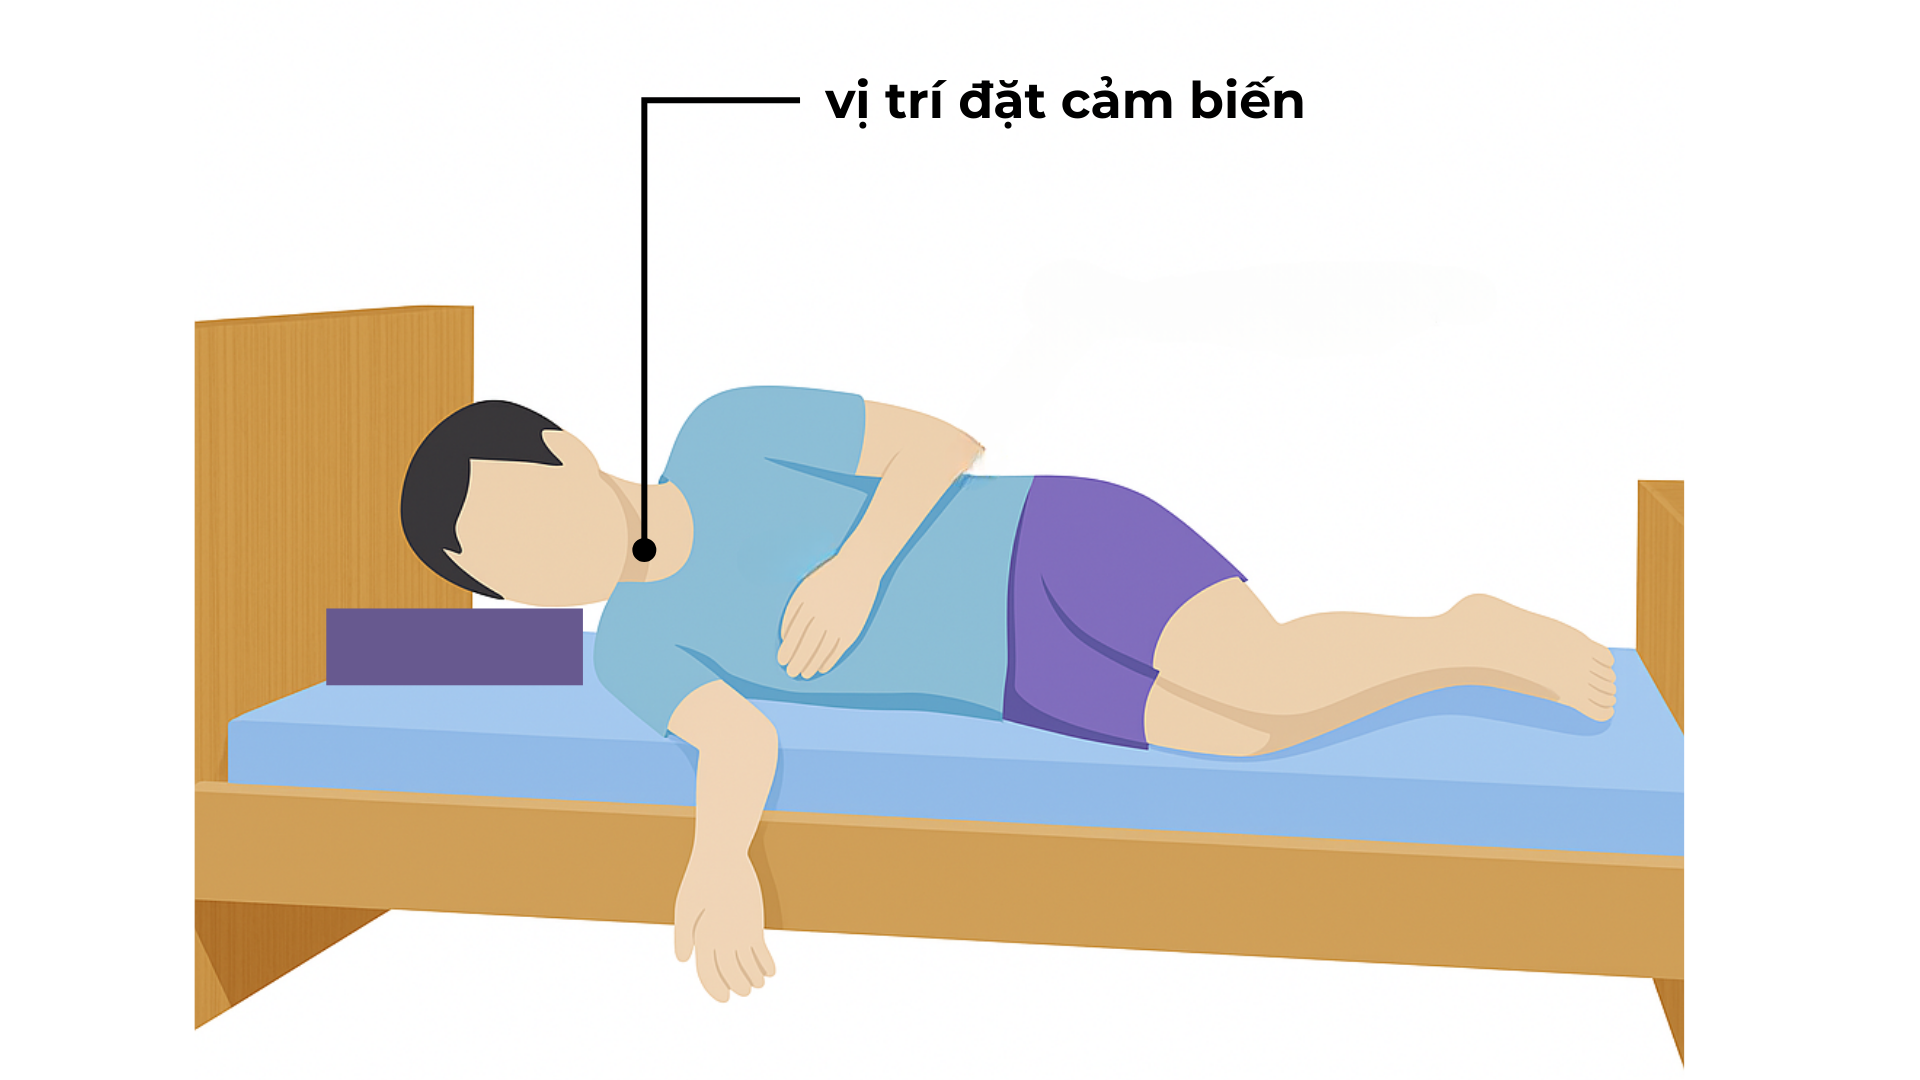
\includegraphics[width=\textwidth]{images/vị trí đặt cảm biến.png}
 		\vspace*{-7mm}
		\caption{Vị trí tối ưu để đặt cảm biến gia tốc}
		\label{position_sensor}
\end{figure}

Trong khuôn khổ luận văn, tác giả đề xuất thiết kế một thiết bị đeo tiếp xúc sử dụng cảm biến gia tốc được đặt tại vị trí xương ức cổ nhằm theo dõi và phân tích tư thế ngủ của người dùng. Vị trí này được lựa chọn không chỉ do tính ổn định trong quá trình ngủ mà còn thuận lợi để tích hợp thêm các cảm biến khác như cảm biến âm thanh và cảm biến nhiệt độ – phục vụ cho các mục tiêu nghiên cứu mở rộng của nhóm. Tín hiệu từ cảm biến gia tốc sẽ được thu thập dưới dạng ba trục không gian (x, y, z), phản ánh chuyển động và hướng trọng lực tương ứng với tư thế cơ thể trong suốt thời gian ngủ. Sau quá trình thu thập, dữ liệu gia tốc sẽ được xử lý sơ cấp bao gồm hiệu chỉnh, lọc nhiễu, và chuẩn hóa nhằm đảm bảo tính chính xác và đồng nhất giữa các mẫu đo. Tiếp theo, các đặc trưng định lượng (features) trong miền thời gian sẽ được trích xuất để phục vụ cho bài toán phân loại tư thế ngủ (ngửa, nghiêng trái, nghiêng phải, sấp). Các đặc trưng này cùng với dữ liệu gốc sẽ được lưu trữ trong hệ thống để phục vụ cho các bước phân tích tiếp theo, bao gồm huấn luyện mô hình học máy hoặc tích hợp với các chỉ số sinh lý khác trong đánh giá rối loạn giấc ngủ, đặc biệt là hội chứng ngưng thở khi ngủ (OSA) hình~\ref{position_sensor}.

\section{Giới thiệu về cảm biến gia tốc nhiều bậc tự do}
Cảm biến gia tốc (accelerometer) là thiết bị được sử dụng phổ biến để đo và phân tích gia tốc của một vật thể. Nhờ khả năng phát hiện sự thay đổi về chuyển động, cảm biến này được ứng dụng rộng rãi trong nhiều lĩnh vực như phát hiện rơi tự do, va chạm, dịch chuyển, rung động, và xoay. Nguyên lý hoạt động chính của cảm biến gia tốc dựa trên định luật II Newton (F = ma), theo đó khi một lực tác động lên một khối lượng, nó sẽ sinh ra gia tốc. Trong cấu trúc cảm biến, sự thay đổi này được ghi nhận thông qua việc chuyển đổi qua lại giữa năng lượng cơ học (sự dịch chuyển của khối lượng) và năng lượng điện (thông qua sự thay đổi điện tích, điện dung hoặc điện áp). Chính khả năng chuyển đổi năng lượng này giúp cảm biến gia tốc hoạt động hiệu quả trong việc giám sát và ghi nhận các trạng thái động học của vật thể.

\begin{figure}[!ht]
		\centering
% 		\setlength{\abovecaptionskip}{1pt plus 3pt minus 2pt}
 		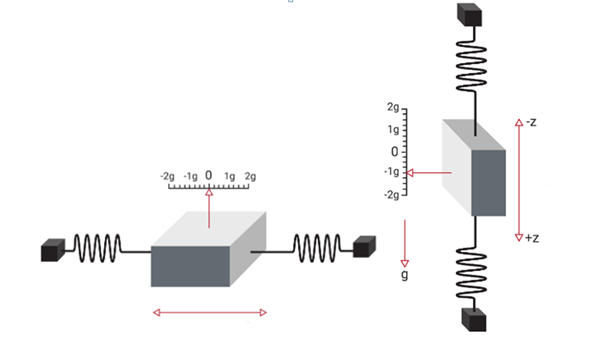
\includegraphics[width=\textwidth]{images/acce.png}
 		\vspace*{-7mm}
		\caption{Nguyên lý cơ bản của cảm biến gia tốc}
		\label{acce}
\end{figure}

Như minh họa trong Hình~\ref{acce}, khi cảm biến gia tốc chịu tác động từ một chuyển động, khối gia trọng (proof mass) sẽ dịch chuyển, làm lò xo kết nối bị biến dạng. Sự biến dạng này tạo ra một lực đàn hồi theo định luật Hooke, tỷ lệ thuận với độ giãn của lò xo. Áp dụng định luật II Newton, ta có mối quan hệ giữa lực, khối lượng và gia tốc như sau:

\begin{equation} F = m \cdot a \Rightarrow a = \frac{k \cdot \Delta l}{m} \end{equation}

Trong đó: \begin{itemize} \item $F$ là lực đàn hồi tác dụng lên khối gia trọng (N) \item $m$ là khối lượng của khối gia trọng (kg) \item $k$ là hệ số đàn hồi của lò xo (N/m) \item $\Delta l$ là độ biến dạng (thay đổi chiều dài) của lò xo (m) \end{itemize}

Phương trình trên cho thấy gia tốc có thể được tính toán gián tiếp thông qua độ biến dạng của lò xo, từ đó cho phép cảm biến gia tốc chuyển đổi dao động cơ học thành tín hiệu điện phục vụ cho việc đo đạc và phân tích chuyển động. Trong hệ tọa độ của cảm biến gia tốc ba trục, trục z thường nằm theo phương vuông góc với mặt phẳng ngang và sẽ chịu thêm tác dụng của trọng lực. Do đó, ở trạng thái cân bằng (khi thiết bị đứng yên và không có chuyển động nào khác), giá trị gia tốc đo được tại trục z sẽ xấp xỉ bằng gia tốc trọng trường $g$ (khoảng 9.81 m/s²). Đặc điểm này có thể được khai thác trong việc hiệu chuẩn cảm biến cũng như xác định tư thế không gian tương đối của thiết bị.

Trong khuôn khổ luận văn này, tác giả tập trung vào việc nghiên cứu và ứng dụng cảm biến gia tốc được chế tạo dựa trên công nghệ vi cơ điện tử (Micro-Electro-Mechanical Systems – MEMS). Đây là một công nghệ tiên tiến cho phép tích hợp các cấu trúc cơ học và linh kiện điện tử ở kích thước vi mô (dưới 10 micromet) trên cùng một chip bán dẫn. Một trong những ưu điểm vượt trội của cảm biến gia tốc MEMS là khả năng gắn trực tiếp lên bo mạch in (PCB), giúp tiết kiệm không gian, giảm chi phí sản xuất và tối ưu hóa thiết kế hệ thống nhúng – đặc biệt phù hợp với các ứng dụng trong thiết bị đeo, điện thoại di động, và hệ thống theo dõi sức khỏe cá nhân.



Hiện nay, có ba loại cảm biến gia tốc MEMS phổ biến, được phân loại dựa trên nguyên lý hoạt động của chúng \cite{Acce}\cite{cambien}:

\begin{itemize}
    \item \textbf{Cảm biến gia tốc dựa trên hiệu ứng điện dung (Capacitive accelerometers)}: Đây là loại cảm biến được sử dụng rộng rãi nhất trong các thiết bị điện tử tiêu dùng như điện thoại thông minh và thiết bị đeo. Nguyên lý hoạt động dựa trên sự thay đổi điện dung giữa các bản cực khi khối gia trọng dịch chuyển dưới tác dụng của gia tốc. Sự thay đổi điện dung này sẽ được chuyển đổi thành tín hiệu điện tương ứng với mức gia tốc.

    \item \textbf{Cảm biến gia tốc dựa trên hiệu ứng áp điện trở (Piezoresistive accelerometers)}: Trong loại cảm biến này, lực hoặc ứng suất cơ học tác động lên cảm biến sẽ làm thay đổi điện trở của vật liệu bán dẫn bên trong. Hiện tượng này – được gọi là hiệu ứng áp điện trở – có đặc tính tuyến tính, trong đó độ biến đổi của điện trở tỷ lệ thuận với lực tác động. Cảm biến loại này thường được ứng dụng trong môi trường có điều kiện khắc nghiệt, do khả năng chịu nhiệt và độ bền cao.

    \item \textbf{Cảm biến gia tốc dựa trên hiệu ứng áp điện (Piezoelectric accelerometers)}: Loại cảm biến này khai thác hiện tượng áp điện, trong đó lực cơ học tác động lên các tinh thể áp điện sẽ tạo ra điện tích. Hiệu ứng áp điện có tính tuyến tính, và lượng điện tích sinh ra tỷ lệ thuận với độ lớn của lực. Cảm biến này phù hợp trong các ứng dụng đo rung động hoặc gia tốc có tần số cao.
\end{itemize}

Mỗi loại cảm biến kể trên đều có những ưu điểm và hạn chế riêng, và việc lựa chọn loại cảm biến phù hợp phụ thuộc vào yêu cầu cụ thể của từng ứng dụng, bao gồm độ chính xác, dải đo, mức tiêu thụ điện năng và điều kiện môi trường hoạt động.



\begin{figure}[H]
	\centering
	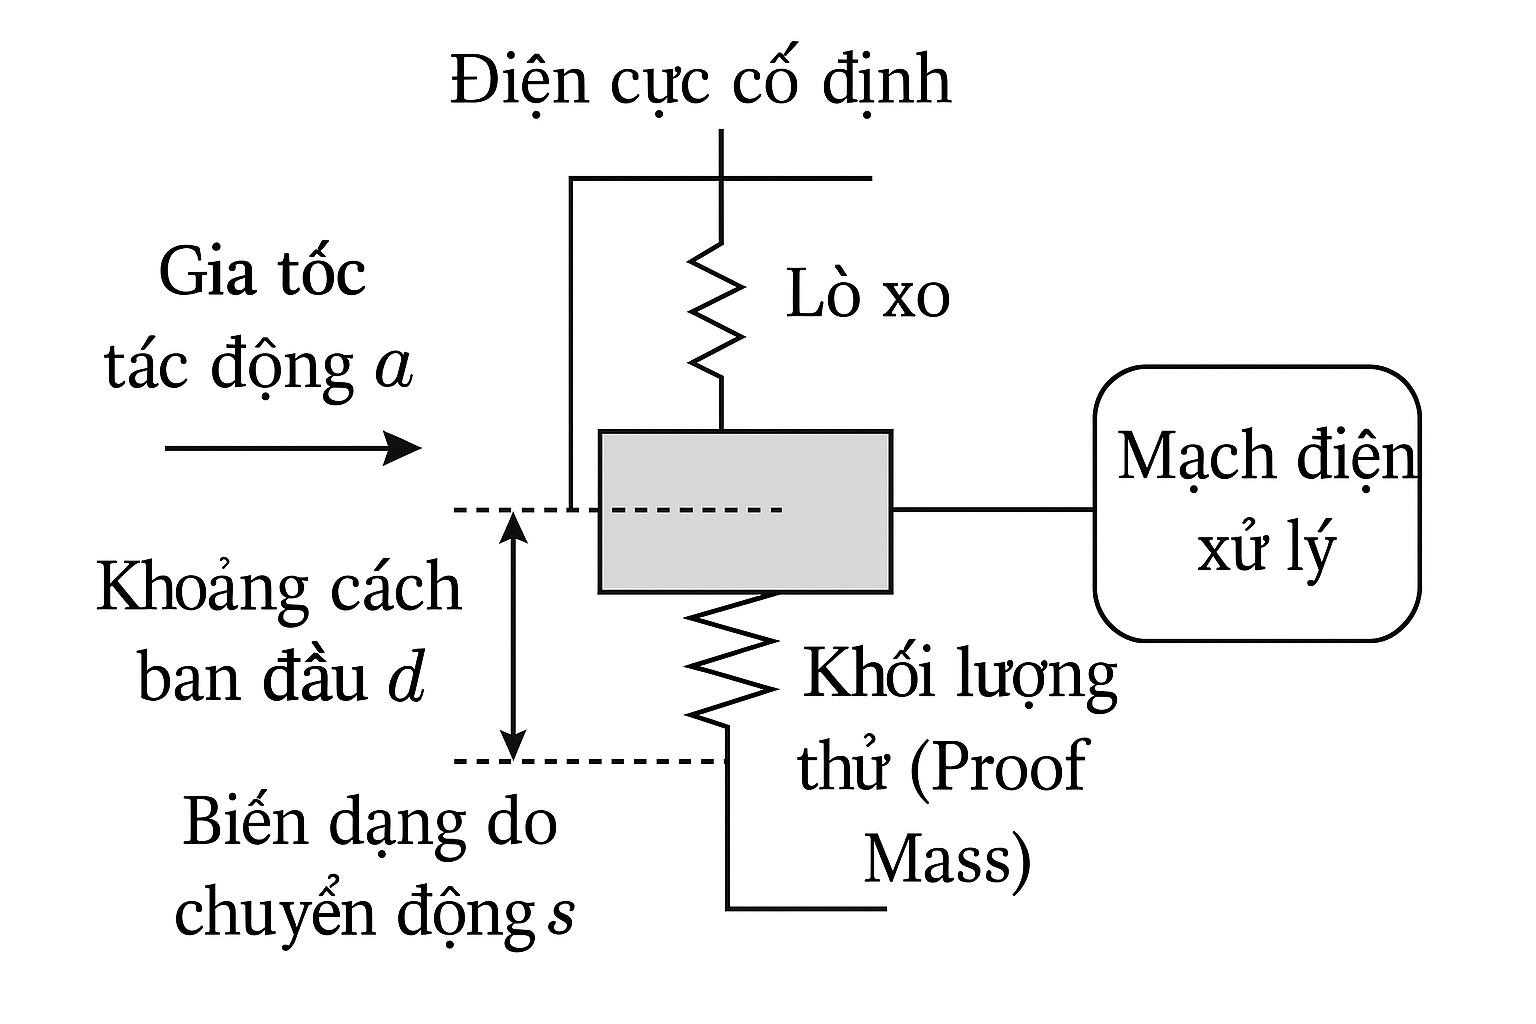
\includegraphics[width=0.7\textwidth]{images/diendung.png}
	\vspace*{-7mm}
	\caption{Cấu trúc cảm biến gia tốc điện dung}
	\label{acce_mems}
\end{figure}




\textbf{Cảm biến gia tốc kiểu điện dung (Capacitive Accelerometers)}


\textit{Nguyên lý hoạt động}: Cảm biến gia tốc kiểu điện dung hoạt động dựa trên nguyên lý biến thiên điện dung giữa các bản cực trong cấu trúc tụ điện khi chịu tác động bởi gia tốc. Cấu hình cơ bản của cảm biến bao gồm một khối lượng vi mô (proof mass) được treo trên hệ thống lò xo vi cơ (MEMS spring system), với một đầu gắn cố định và đầu còn lại liên kết với một bản cực của tụ điện. Khi có một gia tốc tác động theo một phương xác định, khối lượng này sẽ dịch chuyển lệch khỏi vị trí cân bằng, làm thay đổi khoảng cách giữa các bản cực, từ đó gây ra sự biến thiên điện dung. Biến thiên điện dung này được phát hiện thông qua mạch đo nhạy điện dung và được chuyển đổi thành tín hiệu điện tử, tỷ lệ thuận với độ lớn của gia tốc tác động. Quá trình này cho phép cảm biến thu nhận được gia tốc theo thời gian thực với độ chính xác cao. Hình~\ref{acce_mems} minh họa nguyên lý chuyển động và thay đổi điện dung trong cấu trúc cảm biến MEMS điện dung.



\begin{figure} [!]
		\centering
 		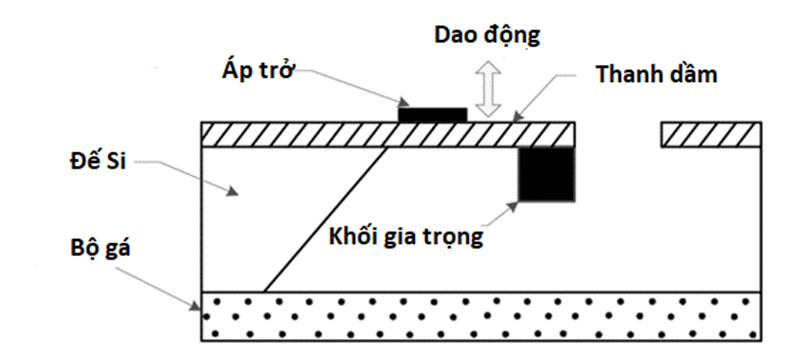
\includegraphics[width=\textwidth]{images/acce_aptro.png}
 		\vspace*{-7mm}
		\caption{Cấu trúc cảm biến áp trở}
		\label{acce_aptro}
  \FloatBarrier
\end{figure}
\textbf{Cảm biến gia tốc kiểu áp điện trở}

Cảm biến kiểu áp điện trở hoạt động dựa trên nguyên lý thay đổi điện trở của các phần tử áp điện trở khi chịu ứng suất cơ học. Trong cấu hình tiêu chuẩn, các phần tử này được gắn trên một thanh dầm (cantilever) liên kết với một khối gia trọng đặt trong môi trường cần đo. Khi có gia tốc tác động, khối gia trọng tạo ra lực quán tính khiến thanh dầm bị biến dạng, từ đó làm thay đổi điện trở của các phần tử cảm biến. Để khuếch đại và cải thiện độ chính xác của tín hiệu, các cảm biến này thường được tích hợp trong cấu trúc mạch cầu Wheatstone. Cách bố trí này cho phép tối đa hóa tín hiệu đầu ra và tăng tỷ số tín hiệu trên nhiễu (Signal-to-Noise Ratio – SNR) của phép đo (xem Hình~\ref{acce_aptro}). Gia tốc kế áp điện trở có ưu điểm nổi bật là khả năng ghi nhận các tín hiệu thay đổi chậm, cũng như hoạt động hiệu quả trong một dải đo rộng. Nhờ đó, thiết bị có thể ghi nhận các dao động có biên độ và tần số cao, rất phù hợp cho các thử nghiệm va chạm hoặc môi trường đo động học phức tạp. Ngoài ra, cảm biến này cũng cho thấy khả năng ổn định tốt trước các thay đổi nhiệt độ của môi trường xung quanh. Tuy nhiên, hạn chế chính của gia tốc kế kiểu này là độ nhạy giảm khi đo tín hiệu yếu, làm giảm hiệu quả trong một số ứng dụng yêu cầu phát hiện dao động nhỏ. Bên cạnh đó, chi phí sản xuất và triển khai cao hơn đáng kể so với các loại gia tốc kế điện dung sử dụng công nghệ MEMS.




\begin{figure} [!]
		\centering
 		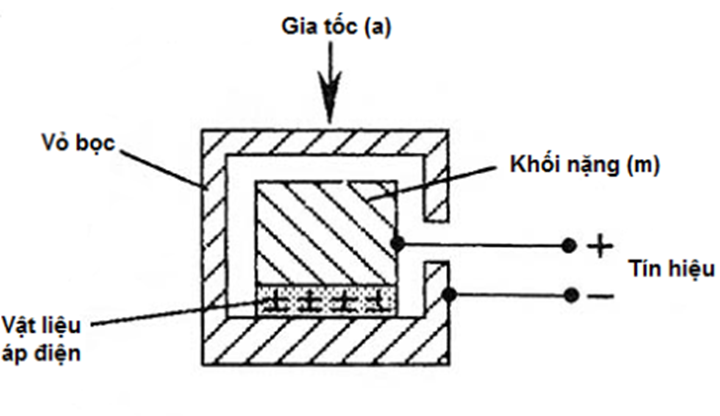
\includegraphics[width=\textwidth]{images/acce_apdien.png}
 		\vspace*{-7mm}
		\caption{Cấu trúc cảm biến áp điện}
		\label{acce_apdien}
  \FloatBarrier
\end{figure}
\textbf{Cảm biến gia tốc kiểu áp điện}

Cảm biến gia tốc kiểu áp điện hoạt động dựa trên hiệu ứng áp điện của một số vật liệu đặc biệt như gốm sứ hoặc thạch anh. Khi các vật liệu này chịu ứng suất cơ học, chúng sẽ bị biến dạng và tạo ra một điện thế trên bề mặt. Lượng điện tích sinh ra tỉ lệ thuận với lực tác dụng lên cảm biến, trong khi chiều cực tính phụ thuộc vào hướng của lực. Một trong những ưu điểm nổi bật của cảm biến gia tốc áp điện so với các loại cảm biến gia tốc khác là khối lượng nhẹ và khả năng đáp ứng tần số rất cao, có thể lên đến khoảng 1 MHz. Đặc điểm này khiến chúng đặc biệt phù hợp để đo các dao động nhanh và ngắn hạn trong các môi trường khắc nghiệt hoặc ứng dụng đòi hỏi độ chính xác cao. Tuy nhiên, cảm biến áp điện vốn có trở kháng đầu ra rất cao và chỉ tạo ra điện áp nhỏ, dễ bị suy giảm tín hiệu nếu không xử lý đúng cách. Do đó, để đảm bảo chất lượng tín hiệu và giảm thiểu hiện tượng sai số do tải (loading error), các bộ khuếch đại chuyển đổi trở kháng chuyên dụng – chẳng hạn như bộ khuếch đại điện tích – thường được tích hợp cùng hệ thống đo (xem Hình~\ref{acce_apdien}).






Đánh giá vị trí của con người trong lúc ngủ không phụ thuộc vào chuyển động quay xung quanh một trục, nên không nhất thiết phải tích hợp thêm con quay hồi chuyển. Thêm vào đó, những điểm nổi bật của cảm biến gia tốc trên công nghệ MEMS như việc ghép nối, tích hợp dễ dàng, trở kháng cao với mạch xử lý tín hiệu tích hợp sẵn cho phép đo biến đổi điện dung, độ nhạy cao, cho phép đáp ứng trong dải tần số đa dạng và đặc biệt là với chi phí phù hợp làm cho cảm biến gia tốc MEMS hay được lựa chọn trong
phát triển thiết bị ngày nay. Trong khuôn khổ luận văn này, với tính chất của chuyển động tư thế ngủ là các chuyển động chậm với biên độ nhỏ, cảm biến MEMS kiểu điện dung được lựa chọn để tiến hành thực nghiệm.

\section{Đánh giá tư thế ngủ sử dụng cảm biến gia tốc, ứng dụng công nghệ trí tuệ nhân tạo trong chẩn đoán OSA}

Vị trí là một trong bảy thông số quan trọng trong mô hình SCOPERA dùng để xác định hội chứng ngưng thở khi ngủ. Phân tích các chuyển động và tư thế trong giấc ngủ không chỉ phản ánh chất lượng giấc ngủ mà còn đóng vai trò thiết yếu trong việc đánh giá chỉ số ngưng thở – AHI. Tư thế ngủ không hợp lý có thể làm thay đổi đặc tính hô hấp và âm thanh thở, từ đó ảnh hưởng đến mức độ nghiêm trọng của OSA. Ở phần lớn bệnh nhân, mức độ nghiêm trọng của hội chứng này có xu hướng tăng rõ rệt khi họ nằm ngửa. Thống kê cho thấy, có đến 60\% bệnh nhân ghi nhận chỉ số AHI tăng gấp đôi khi ngủ ở tư thế nằm ngửa – tình trạng này được gọi là hội chứng ngưng thở khi ngủ phụ thuộc tư thế (positional Obstructive Sleep Apnea – pOSA) \cite{Unat1391}.

Vì lý do đó, việc ghi nhận và phân tích tư thế ngủ đóng vai trò then chốt trong quá trình phát triển các thiết bị hỗ trợ đánh giá giấc ngủ một cách toàn diện và chính xác. Thông tin về tư thế ngủ không chỉ góp phần làm rõ mối liên hệ giữa vị trí cơ thể và mức độ nghiêm trọng của chứng ngưng thở khi ngủ, mà còn hỗ trợ cá nhân hóa phương pháp điều trị cho từng bệnh nhân. Tư thế ngủ của con người thường được phân loại thành bốn nhóm chính: nằm ngửa, nghiêng trái, nghiêng phải và nằm sấp (Hình~\ref{4_tuthe}) \cite{4_ngu}. Việc phân biệt rõ ràng các tư thế này giúp nâng cao độ chính xác trong việc phân tích ảnh hưởng của tư thế đến các chỉ số sinh lý trong giấc ngủ.

\begin{figure}
		\centering
 		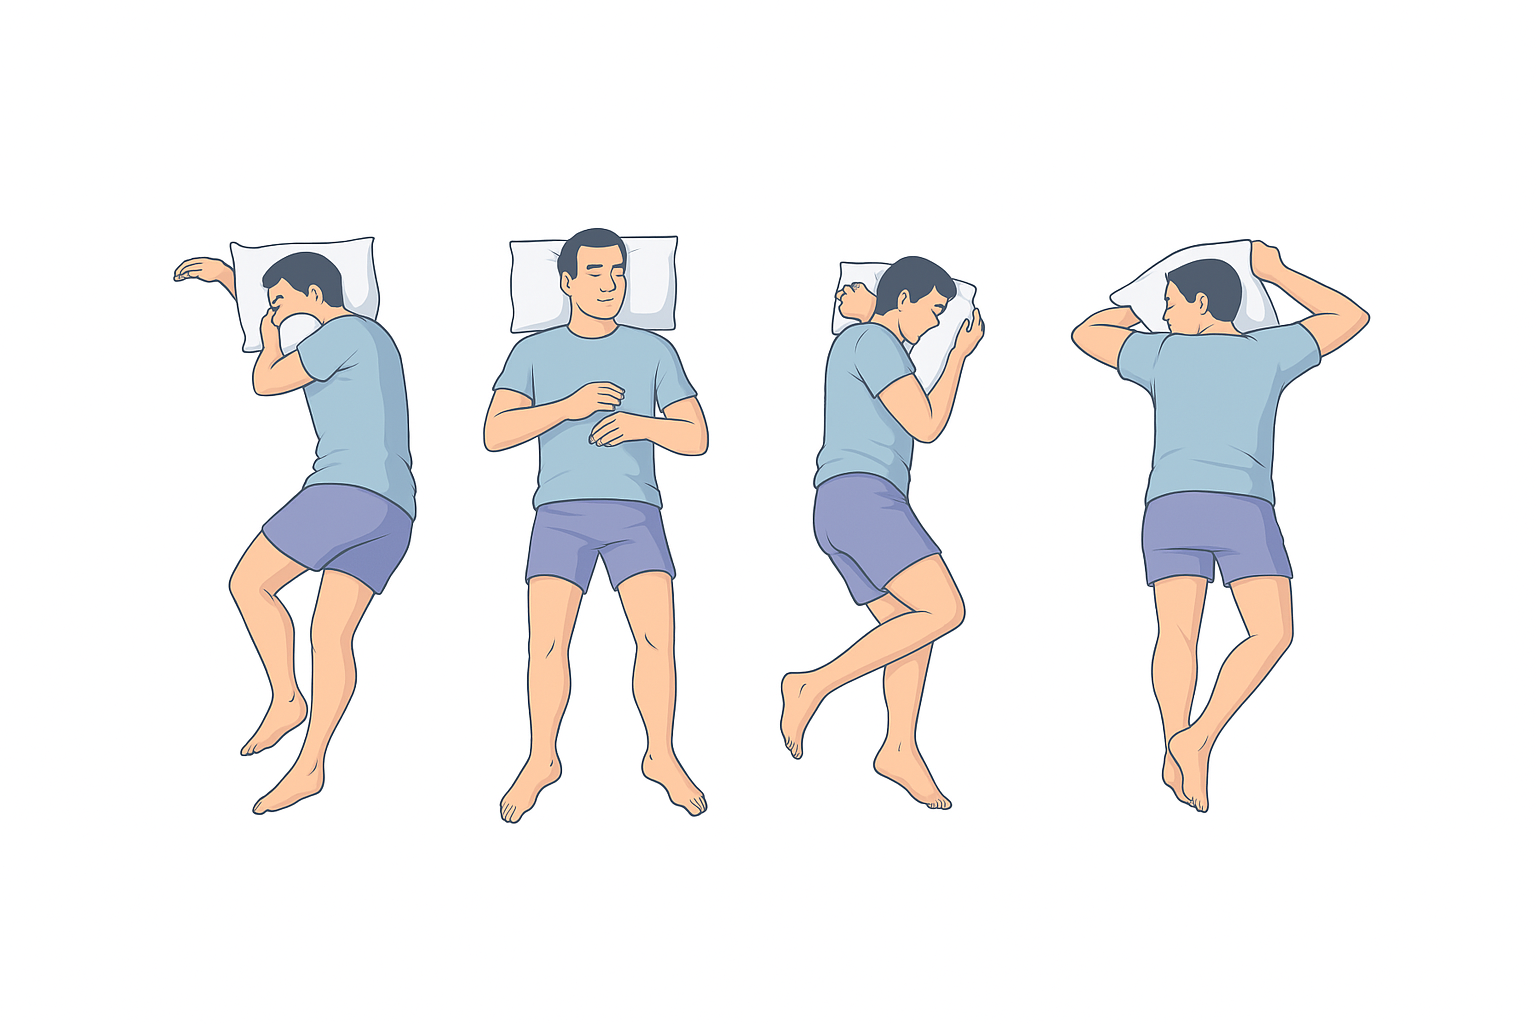
\includegraphics[width=\textwidth]{images/4ngu.png}
 		\vspace*{-7mm}
		\caption{Các tư thế ngủ cơ bản của con người}
		\label{4_tuthe}
\end{figure}

Tư thế ngủ có ảnh hưởng rõ rệt đến mức độ nghiêm trọng của hội chứng ngưng thở khi ngủ tắc nghẽn (OSA), do đó việc phân tích chi tiết từng tư thế là điều cần thiết trong các nghiên cứu và ứng dụng lâm sàng. Các tư thế ngủ khác nhau có thể tác động trực tiếp đến cơ chế tắc nghẽn đường thở, làm thay đổi tần suất và mức độ nghiêm trọng của các đợt ngưng thở. Trong số đó, các tư thế nằm nghiêng (bao gồm nghiêng trái và nghiêng phải) được ghi nhận là có khả năng cải thiện triệu chứng OSA ở nhiều bệnh nhân nhờ hạn chế tình trạng sụp đổ của đường thở trên so với tư thế nằm ngửa. Việc duy trì tư thế nằm nghiêng giúp giảm hiện tượng ngáy và hỗ trợ lưu thông khí thở tốt hơn. Tuy nhiên, sự khác biệt rõ ràng về hiệu quả giữa tư thế nghiêng trái và nghiêng phải vẫn chưa được xác định chắc chắn, và cần được đánh giá dựa trên đặc điểm cá nhân và bệnh lý kèm theo của từng người bệnh. Tư thế nằm sấp có thể làm giảm nguy cơ tắc nghẽn đường thở do trọng lực kéo các mô mềm, bao gồm cả lưỡi, về phía trước. Tuy nhiên, tư thế này không phù hợp với mọi đối tượng, đặc biệt là những người có thói quen che mặt hoặc miệng bằng gối, vì có thể làm hạn chế luồng khí hít vào. Ngoài ra, ở những bệnh nhân có vấn đề về cột sống cổ, tư thế nằm sấp có thể gây ra căng thẳng không cần thiết và làm trầm trọng thêm tình trạng cơ xương khớp. Ngược lại, tư thế nằm ngửa thường liên quan đến nguy cơ cao hơn đối với các đợt ngưng thở khi ngủ. Trong tư thế này, các mô mềm của đường thở trên – đặc biệt là lưỡi – dễ bị trọng lực kéo lùi về phía sau, gây hẹp hoặc tắc nghẽn đường thở. Do đó, nằm ngửa được xem là tư thế dễ làm trầm trọng thêm OSA và nên được cân nhắc hạn chế trong chiến lược quản lý bệnh \cite{LANDRY2023101847}.

Sự phát triển nhanh chóng của trí tuệ nhân tạo (AI) trong lĩnh vực y học đã mở ra nhiều hướng tiếp cận mới trong việc đánh giá tư thế ngủ và chẩn đoán OSA. Các hệ thống AI đang dần chứng minh hiệu quả vượt trội trong việc xử lý dữ liệu cảm biến lớn và phức tạp, từ đó cung cấp các phân tích chính xác về hành vi giấc ngủ của bệnh nhân. Các mô hình học máy được huấn luyện trên tập dữ liệu cảm biến từ accelerometer, gyroscope hoặc thiết bị đeo thông minh có thể tự động phân loại các tư thế ngủ theo thời gian thực, với độ chính xác lên đến trên 90\% trong nhiều nghiên cứu gần đây \cite{Sleep_Posture_Detection}\cite{Vu2025SleepPosition}\cite{HOANG2025116309}. 

Nhờ vào khả năng học và tự hiệu chỉnh, các thuật toán này có thể phân biệt hiệu quả giữa các trạng thái nằm nghiêng trái, nghiêng phải, nằm ngửa và nằm sấp – ngay cả khi có sự biến đổi nhẹ về góc độ hoặc cử động cơ thể. Hơn nữa, AI còn cho phép tích hợp thông tin về tư thế ngủ với các chỉ số sinh lý khác như nhịp tim, nhịp thở, SpO₂ và dữ liệu âm thanh để xây dựng mô hình chẩn đoán OSA đa chiều. Việc kết hợp các nguồn dữ liệu này giúp phát hiện chính xác các giai đoạn ngưng thở và giảm thở, đồng thời đánh giá được mức độ ảnh hưởng của từng tư thế đến tình trạng hẹp đường thở trong khi ngủ. Đây là một bước tiến quan trọng hướng đến cá nhân hóa chẩn đoán và điều trị OSA – điều mà các phương pháp truyền thống như đa ký giấc ngủ (polysomnography) còn nhiều hạn chế do chi phí cao và điều kiện thực hiện phức tạp. Đặc biệt, các hệ thống AI có thể được triển khai trong các thiết bị đeo thông minh tại nhà, hỗ trợ theo dõi lâu dài và liên tục mà không gây xâm lấn hay gián đoạn giấc ngủ. Nhờ đó, dữ liệu thu thập được phản ánh chính xác hơn về hành vi giấc ngủ trong môi trường tự nhiên của người bệnh, từ đó nâng cao giá trị lâm sàng của các kết quả phân tích. Ngoài ra, sự tích hợp AI trong các thiết bị di động, cùng với công nghệ điện toán biên (edge computing), có thể cho phép xử lý dữ liệu tại chỗ và phản hồi thời gian thực – mở ra tiềm năng to lớn trong việc sàng lọc, theo dõi và cá nhân hóa chiến lược quản lý OSA.

















% \section{Cơ chế giả lập hành vi\label{mock_mechanism}} 
% % Từ khóa sử dụng: mock, mocking, mock data, HTTP Request, caller, callee, API method
% \begin{lstlisting}[float,language=JavaScript,caption={Ví dụ phương thức API ($searchMasterData()$) gọi đến hai phương thức khác, trong đó có một phương thức ($get()$) cần được tạo hàm giả khi thực thi kiểm thử}, label=api_example,captionpos=b]
async get(req: RequestModel): Promise<any> { //Accessing database (*@\label{declare_get_method}@*)
    return await this.httpService
      .post<any>(Utils.join(this.apiUrl, this.config.CORE_GET), req) (*@\label{call_http_service}@*)
      .toPromise(); (*@\label{get_method_toPromise}@*)}
      
@Post('search') //The tested API
async searchMasterData(@Body() body: RequestModel<BaseDto>): Promise<any> { (*@\label{declare_api_method}@*)
    // Hidden code...
    await this.checkRequired(body.condition['type']); (*@\label{lst_exp_check_require}@*)
    let reqCon = body.condition;
    switch (reqCon['type']) { (*@\label{lst_exp_switch_stmt}@*)
        case "MASTER":(*@\label{lst_exp_case_branch}@*)
            if (!(type of reqCon["keyword"] === "string") (*@\label{lst_exp_if_stmt}@*)) {
                (*@\label{lst_exp_keyword_branch}@*)return ResponseModel(RESULT_STATUS.ERROR);}
            const ret = await this.get(reqCon);(*@\label{lst_exp_start_uncover}@*)
            if (ret.status == 200) { (*@\label{lst_exp_200}@*) 
                // Hidden code... (*@\label{lst_exp_hidden_code}@*)
                return  new ResponseModel(RESULT_STATUS.OK, ret); (*@\label{lst_exp_end_uncover}@*)}
            return new ResponseModel(RESULT_STATUS.ERROR);(*@\label{lst_exp_return_error}@*)
        //Other cases....
        default: (*@\label{lst_exp_default_branch}@*)
            return new ResponseModel(RESULT_STATUS.ERROR);}
}

checkRequired(s: string): Promise<any> { //A normal method (*@\label{declare_check_required_method}@*)
    if (s == null (*@\label{check_null_equal}@*)) {
        this.errors.push("error message");}
}
\end{lstlisting}

% \begin{lstlisting}[float,language=JavaScript,caption={An example presents one caller ($search()$) and two callees ($get()$ and $check()$), in which the first callee ($get()$) needs to be mocked.}, label=api_example,captionpos=b]
% @Post('search')
% async search(body: Dto): any { (*@\label{declare_api_method}@*)
%     this.check(body['type']); (*@\label{lst_exp_check_require}@*)
%     switch (body['type']) { (*@\label{lst_exp_switch_stmt}@*)
%         case "MASTER":(*@\label{lst_exp_case_branch}@*)
%             if (body["keyword"] is not a string)(*@\label{lst_exp_if_stmt}@*)) 
%                 return ...
%             const ret = await this.get(reqCon);(*@\label{lst_exp_start_uncover}@*)
%             if (ret.status == 200 (*@\label{lst_exp_200}@*)) 
%                 return ... (*@\label{lst_exp_end_uncover}@*)
%             else  return ...(*@\label{lst_exp_return_error}@*)
%     }
% }
% //A method gets data from database
% async get(req): any (*@\label{declare_get_method}@*){ ...}
% check(s: string): any (*@\label{declare_check_required_method}@*) {  //A normal callee
%     if (s == null (*@\label{check_null_equal}@*))  
%         this.errors.push("error message");}
% \end{lstlisting}
% % return await this.httpService
% %       .post<any>(Utils.join(this.apiUrl, this.config.CORE_GET), req) (*@\label{call_http_service}@*).toPromise(); (*@\label{get_method_toPromise}@*)
% \begin{lstlisting}[float,language=JavaScript,caption=An example of mocking $get()$ method, label=mock_example,captionpos=b]
% it("first test", (done) => {
%     // generated input
%     const body = {...}; (*@\label{input_declaration}@*)
%     // initialize mock data
%     const response: AxiosResponse < any > = {(*@\label{mock_declare_response}@*) status: 200,
%         data: {}, headers: {}, statusText: 'OK', config: {url:'x'}};
%     // set mock data to method accessing database
%     jest.spyOn(controller_class, "get").mockResolvedValue(response); (*@\label{mock_spy}@*)
%     // call the tested API
%     return request(server).post("/search") (*@\label{begin_test_driver}@*)
%     .send(body)  (*@\label{end_test_driver}@*).expect(201).then(res => {...})
% });
% \end{lstlisting}
% Quá trình thực thi kiểm thử cần được đảm bảo là độc lập và nhanh chóng \cite {clean_coder}. Để làm được điều này, chúng ta có thể áp dụng cơ chế giả lập hành vi cho một số hàm hoặc phương thức tương tác với thành phần bên ngoài như cơ sở dữ liệu, dịch vụ bên thứ ba, v.v. Cơ chế giả lập hành vi (\textit{\gls{mocking}}) được sử dụng để cài đặt các hàm hoặc phương thức với các hành vi mới. Thay vì truy cập các tài nguyên từ xa như trang Web hoặc cơ sở dữ liệu, các nhà phát triển hoặc người kiểm thử có thể thay thế hành vi mới của hàm/phương thức bằng cách sử dụng dữ liệu giả (\textit{\gls{mockdata}}). \Gls{mockdata} được cố ý chèn vào một phần trong mã nguồn. Nó thường được sử dụng như là kết quả của các phương thức hoặc hàm. Nó có nghĩa là những phương thức/hàm này được thay đổi hành vi để phù hợp với việc thực thi kiểm thử. Để đơn giản, thuật ngữ \textit {``\gls{mocked_method}"} dùng để chỉ một phương thức kết nối với các tài nguyên từ xa và phải được thay đổi hành vi. Sử dụng cơ chế \gls{mocking} có hai lợi ích chính là quá trình kiểm thử trở nên nhanh chóng và độc lập, điều này cần có trong các nguyên tắc FIRST \cite {clean_coder}. 

% Ưu điểm đầu tiên của việc sử dụng cơ chế \gls{mocking} là nhanh chóng. Kỹ thuật này làm giảm chi phí tính toán để thực thi dữ liệu thử nghiệm. Nếu không áp dụng cách thức này, việc kết nối với các tài nguyên từ xa có thể gặp phải một số sự cố do kết nối mạng kém hoặc không khả dụng. Thay vì đợi phản hồi từ các tài nguyên từ xa, các phương thức có thể trả về nhanh chóng \gls{mockdata}. Một lợi thế khác của việc sử dụng cơ chế \gls{mocking} là đảm bảo tính độc lập. Nó giúp duy trì tính nhất quán của cơ sở dữ liệu khi thực thi dữ liệu thử nghiệm nhiều lần. Khi một ứng dụng Web doanh nghiệp được triển khai, hầu hết các API có thể yêu cầu một số thay đổi tương tác với cơ sở dữ liệu. Tuy nhiên, trong môi trường thử nghiệm, việc thực thi thử nghiệm không được tác động đến cơ sở dữ liệu để duy trì tính nhất quán của dữ liệu gốc. Thay vì thực hiện hành vi thực tế, các phương thức có thể trả về \gls{mockdata} ngay lập tức. Do đó, việc thực thi thử nghiệm sẽ không bao giờ thực hiện bất kỳ cập nhật nào đối với cơ sở dữ liệu.

% Để làm rõ hơn cơ chế \gls{mocking} được sử dụng như thế nào trong thực tế, ví dụ trong Mã nguồn~\ref{api_example} và Mã nguồn~\ref{mock_example} thể hiện một trường hợp cần phải dùng tới cơ chế này. Ví dụ đầu tiên Mã nguồn~\ref{api_example} có API $``/search"$ lấy dữ liệu từ tài nguyên bên ngoài bằng cách gọi phương thức $get()$ (dòng \ref{lst_exp_start_uncover}). Bên cạnh đó, Mã nguồn~\ref{mock_example} trình bày một ca kiểm thử có sử dụng \gls{mocking} cho API $``/search"$  trong Mã nguồn~\ref{api_example}. 
% Để đơn giản hóa, nếu phương thức $m_1$ gọi phương thức $m_2$, $m_1$ và $m_2$ tương ứng được gọi là
% \textit{``caller"} và \textit{``callee"}.

% \begin{lstlisting}[float,language=JavaScript,caption=Ví dụ áp dụng \gls{mocking} đối với mã nguồn dự án sử dụng framework NestJS, label=mock_example,captionpos=b]
it("first test", (done) => {
    const body = {...}; (*@\label{input_declaration}@*)  // input generated by the two methods
    const response: AxiosResponse < any > = {(*@\label{mock_declare_response}@*)// initialize mock data
        data: {}, headers: {}, config: {},
        status: 200, statusText: 'OK'};
    // set mock data to method accessing database
    jest.spyOn(controller_class, "get")
        .mockResolvedValue( of(response).toPromise()); (*@\label{mock_spy}@*)
    // send request data to the tested API
    return request(server)
    .post("/search") (*@\label{begin_test_driver}@*)
    .send(body)  (*@\label{end_test_driver}@*)
    .expect(201).then(res => {
        console.log(res.body);
        expect(res.body).not.toBeNull();
        done();
    })
});
\end{lstlisting}
% Thứ nhất, Mã nguồn~\ref{api_example} thể hiện một ví dụ cần phải sử dụng cơ chế \gls{mocking} khi thực thi kiểm thử. Ví dụ này có một phương thức chính ($searchMasterData()$) và hai phương thức phụ ($get()$ và $checkRequired()$). Chúng là những đại diện điển hình của mã nguồn dự án được sử dụng làm thực nghiệm trong Mục~\ref{experiment_section} Mỗi phương thức đều có những đặc điểm riêng biệt. Đầu tiên, phương thức chính ($searchMasterData()$) được đánh dấu với ký hiệu $@Post("search")$ cung cấp bởi thư viện NestJS (dòng \ref{declare_api_method}). Điều này có nghĩa là phương thức này tương ứng với một API. API này có thể được lựa chọn nằm trong môi trường kiểm thử. Phương thức này gọi tới hai phương thức khác: phương thức $get()$ để lấy kết quả phản hồi từ một cơ sở dữ liệu (dòng \ref{lst_exp_start_uncover}) và phương thức thứ hai $checkRequired()$ để kiểm tra lại tính hợp lệ của dữ liệu đầu vào (dòng \ref{lst_exp_check_require}). 
% Ngoài ra, phương thức đầu tiên ($get()$) kết nối với máy chủ cơ sở dữ liệu từ xa bằng cách sử dụng đối tượng $httpService$ với phương thức $post()$ để gửi POST Request (dòng \ref{call_http_service}). Phương thức này cần được thiết lập hành vi giả trong tệp kiểm thử. Liên quan đến vấn đề này, kiểu trả về của phương thức này có cấu trúc lớp $AxiousResponse$ bao gồm một số thuộc tính như là $data, headers,config, status$, và $statusText$ \footnote{https://github.com/axios/axios\#response-schema}. Những thuộc tính này cần được cung cấp trong \textit{mock data} để thỏa mãn yêu cầu về kiểu trả về của phương thức. Cuối cùng, phương thức $checkRequired()$ là một phương thức bình thường có nhiệm vụ là kiểm tra sự tồn tại của một thuộc tính đặc biệt trong đầu vào. Vì vậy, nó không cần thiết phải áp dụng cơ chế \gls{mocking} trong tệp thực thi kiểm thử.
% % The caller is an API that needs to be tested and it calls the callee which connects to a remote database.
% % As a result, the consistency of data could be impacted during test execution. Therefore, the actual implementation of this callee has to be replaced by using mock data

% Thứ hai, Mã nguồn~\ref{mock_example} trình bày ví dụ một tập lệnh cho một ca kiểm thử cho API $@Post("search")$ trong Mã nguồn~\ref{api_example}. Tập lệnh này có sử dụng cơ chế \gls{mocking} cho phương thức truy cập đến có sở dữ liệu  $get()$. Đây là ví dụ một khối lệnh viết bằng ngôn ngữ Typescript để xây dựng một ca kiểm thử cho một API trong ứng dụng NestJS. API được gọi với đầu là một HTTP Request có chứa dữ liệu kiểm thử ảnh hưởng đến luồng thực thi của chương trình. Khối lệnh này có cấu trúc bao gồm ba phần: Khai báo giá trị đầu vào (dòng \ref{input_declaration}), khai báo \textit{mock data}  (dòng \ref{mock_declare_response}-\ref{mock_spy}), và lời gọi API (dòng \ref{begin_test_driver}-\ref{end_test_driver}).
% Như đã đề cập ở trước đó, phương thức $get()$ kết nối tới máy chủ cơ sở dữ liệu và cần được thiết lập hành vi thay thế. Vì vậy, \textit{mock data} được cung cấp (dòng \ref{mock_declare_response}-\ref{mock_spy}). Ở khía cạnh đầu tiên, nếu cơ chế \gls{mocking} không được áp dụng, phương thức $get()$ sẽ gửi một POST Request tới máy chủ từ xa dẫn đến tốn thêm thời gian để đợi phản hồi. Thêm vào đó, nếu máy chủ đang không khả dụng, giá trị thuộc tính $status$ của biến $ret$ trong Mã nguồn~\ref{api_example} luôn luôn khác $200$. Điều này có nghĩa là biểu thức điều kiện $ret.status == 200$ luôn luôn nhận giá trị $false$ (dòng \ref{lst_exp_200} trong Mã nguồn~\ref{api_example}), khiến một số câu lệnh không thể được thực thi khi chạy kịch bản kiểm thử (dòng \ref{lst_exp_hidden_code},\ref{lst_exp_end_uncover} trong Mã nguồn~\ref{api_example}). 
% Ở khía cạnh khác, cơ chế \gls{mocking} cần được áp dụng để đảm bảo cơ sở dữ liệu không bị ảnh hưởng (dòng \ref{mock_spy}). \Gls{mockdata} của phương thức $get()$  là giá trị của biến $response$ bao gồm tất cả những thuộc tính cần thiết như là $data, headers,config, status$, và $statusText$ (dòng \ref{mock_declare_response}). Những giá trị này sẽ giúp chương trình thực thi nhiều câu lệnh hơn. 

% Trên thực tế, \gls{mockdata} thường được các nhà phát triển hoặc người thử nghiệm sửa đổi dựa trên kinh nghiệm của họ. Bởi vì luồng thực thi có thể phụ thuộc vào cách các phương thức được giả lập, \gls{mockdata} có thể ảnh hưởng đến phạm vi bao phủ. Do đó, các nhà phát triển hoặc người kiểm tra cần phải hiểu rõ ràng về mã nguồn để thiết lập \gls{mockdata} phù hợp nhằm đạt được độ phủ cao hơn.

% \section{Kiểm thử ứng dụng Web}
% Cách đơn giản nhất để kiểm thử một ứng dụng Web là kiểm thử viên sẽ thực hiện các thao tác nhấp chuột thủ công trên giao diện của hệ thống và đánh giá cách ứng dụng phản hồi. Đây là phương pháp kiểm thử hộp đen \cite{black_box_testing} vì kiểm thử viên không cần biết chi tiết nội hàm của chương trình ứng dụng. Họ chỉ cần quan tâm xem với một đầu vào cụ thể, ứng dụng có thực thi hành vi đúng như đặc tả hay không. Phương pháp kiểm thử này dễ dàng thực hiện được vì không cần bất cứ thiết lập nào trước đó. Tuy nhiên, nó có thể bị ảnh hưởng bởi những lỗi liên quan đến người thực hiện kiểm thử. Ngoài ra, quá trình này cũng tốn rất nhiều thời gian và công sức khi mà tổ hợp các kịch bản người dùng thực hiện trên giao diện là một con số rất lớn. Điều này trở nên thách thức hơn khi mã nguồn luôn luôn có sự thay đổi, quá trình kiểm thử hồi quy cần được thực hiện liên tục để kiểm tra lại các thành phần trước đó vẫn hoạt động đúng như ban đầu. Vì vậy, việc kiểm thử đầy đủ nếu chỉ dựa vào kiểm thử thủ công trên giao diện là không hiệu quả.

% Thay vì kiểm thử viên nhấp chuột thủ công để kiểm thử hệ thống, họ có thể viết các dữ liệu kiểm thử sử dụng trình điều khiển Web. Trình điều khiển Web thực hiện lần lượt các bước mô tả trong dữ liệu kiểm thử và kiểm tra hành vi của hệ thống. Quá trình thực thi các dữ liệu kiểm thử này có thể được tự động hóa cho nên nó có thể tiết kiệm thời gian cho kiểm thử viên ở giai đoạn thực thi hệ thống. Những dữ liệu kiểm thử có thể được tái sử dụng cho những lần kiểm thử hồi quy sau này. Tuy nhiên, về bản chất, việc xây dựng và viết mã lệnh cho các dữ liệu kiểm thử vẫn phải thực hiện thủ công. Đây là công việc rất tốn thời gian và nguồn nhân lực, đòi hỏi lập trình viên có kiến thức về trình điều khiển Web. Để kiểm thử đầy đủ cho một ứng dụng Web, số lượng dữ liệu kiểm thử là rất lớn. Vì vậy, trong thực tế, danh sách dữ liệu kiểm thử thường không đầy đủ dẫn đến một số lỗi tiềm ẩn trong chương trình không thể phát hiện và thường bị bỏ qua.

% Với những hạn chế như đã được để cập ở trên, việc sinh dữ liệu kiểm thử cần được tự động hóa sao cho đảm bảo tính hiệu quả để tiết kiệm thời gian và chi phí cho doanh nghiệp phát triển phần mềm. Đây cũng là một trong những mảng nghiên cứu khá là quan trọng, dành được nhiều sự quan tâm của các nhà nghiên cứu trong lĩnh vực công nghệ phần mềm. Việc kiểm thử cho ứng dụng Web hiện nay gặp phải một số thách thức \cite{web_testing_1, web_testing_2}. Hiện tại, quá trình nghiên cứu các phương pháp tự động hóa sinh dữ liệu kiểm thử cho ứng dụng Web cũng đã đạt được một số kết quả nhất định. Có thể kể đến một số dự án nổi bật như là Artemis\cite{artermis}, Crawljax \cite{crawljax}, và SymJS \cite{symjs}. Artemis là một công cụ hỗ trợ kiểm thử tự động cho ứng dụng Javascript, tập trung vào các ứng dụng đơn trang. Công cụ này sử dụng một số hằng số và giá trị ngẫu nhiên để sinh ra đầu vào cho dữ liệu kiểm thử. Tiếp theo, Crawljax là một công cụ thu thập thông tin và kiểm thử cho các ứng dụng Web Ajax. Nó có thể thực hiện trên ứng dụng Web có quy mô lớn nhưng chỉ sinh ra các giá trị ngẫu nhiên cho đầu vào. Cả hai công cụ này mặc dù có thể sinh dữ liệu kiểm thử tự động cho ứng dụng Web nhưng bộ dữ liệu kiểm thử không hiệu quả vì không phân tích sâu đến nội hàm các xử lý lô-gic của thành phần kiểm thử. Khác với hai công cụ trước đó, SymJS là công cụ có phân tích mã nguồn của thành phần kiểm thử trong ứng dụng, thu thập các toán tử có điều kiện và thực thi tượng trưng để sinh ra bộ các đầu vào đi qua các đường đi khác nhau trong chương trình. Tuy nhiên, hiện tại công cụ này mới chỉ hỗ trợ mã nguồn JavaScript phía người dùng. Có thể nói rằng SymJS đã bước đầu nghiên cứu các phương pháp kiểm thử hộp trắng cho các ứng dụng Web. Phương pháp kiểm thử hộp trắng từ lâu đã được ứng dụng để sinh tự động dữ liệu kiểm thử ở nhiều ngôn ngữ lâu đời như Java, C++, C\#, v.v. và đã đạt được một số kết quả khả quan. Bộ dữ liệu kiểm thử được sinh ra bởi phương pháp này có thể đạt độ phủ cao, thực thi qua nhiều thành phần có trong chương trình. Tuy nhiên, phương pháp này cũng vẫn tồn tại mộ số nhược điểm nhất định và chưa thể coi như là một giải pháp tổng thể cho tất cả các mã nguồn dự án phần mềm. Việc áp dụng phương pháp này như thế nào thì phải phụ thuộc vào bài toán cụ thể hoặc đặc trưng của mã nguồn được áp dụng. Thời điểm hiện tại vẫn chưa có nhiều nghiên cứu ứng dụng phương pháp kiểm thử hộp trắng cho ứng dụng Web.

% \section{Kiểm thử hộp trắng}
% Phương pháp được đề xuất trong luận văn này xây dựng dựa trên phương pháp kiểm thử dòng điều khiển. Đây là một trong những phương pháp kiểm thử hộp trắng đảm bảo tất cả các thành phần có trong mã nguồn đều được thực thi. Cụ thể, kiểm thử hộp trắng là phương pháp sinh dữ liệu kiểm thử dựa trên việc phân tích cấu trúc bên trong của mã nguồn \cite{software_testing, white_box_testing_2}. Nếu kiểm thử hộp đen cho phép phát hiện lỗi/khiếm khuyết có thể quan sát được thì kiểm thử hộp trắng có thể phát hiện những lỗi/khiếm khuyết tiềm ẩn bên trong chương trình/đơn vị phần mềm. Các lỗi này thường rất khó có thể phát hiện bằng kiểm thử hộp đen, tuy nhiên điều này không có nghĩa là kiểm thử hộp đen là không quan trọng. Mỗi phương pháp đều có những ưu nhược điểm và mục đích khác nhau, thường xuyên được sử dụng kết hợp với nhau trong quy trình kiểm thử nhằm đảm bảo phần mềm có chất lượng tốt nhất. Kiểm thử hộp trắng có các dữ liệu kiểm thử được sinh ra từ mã nguồn bằng các kỹ thuật phân tích phức tạp. Vì vậy, để có thể áp dụng được phương pháp này, các kỹ thuật viên không chỉ cần nắm rõ giải thuật mà còn cần có các kỹ năng và kiến thức tốt về ngôn ngữ lập trình, hiểu rõ được mã nguồn mới có thể đưa ra những cách giải quyết phù hợp. Do đó, việc áp dụng các phương pháp kiểm thử hộp trắng thường tốn nhiều thời gian và công sức, đặc biệt khi thành phần kiểm thử có kích thước lớn. Với lý do như vậy, các phương pháp kiểm thử hộp trắng thường được áp dụng trong pha kiểm thử đơn vị.

% Hai phương pháp được sử dụng trong kiểm thử hộp trắng là kiểm thử dòng điều khiển (Control Flow Testing - CFT) và kiểm thử dòng dữ liệu (Data Flow Testing - DFT) \cite{whitebox-testing}. Phương pháp kiểm thử dòng điều khiển tập trung kiểm thử tính đúng đắn của các giải thuật sử dụng trong thành phần cần kiểm thử. Phương pháp kiểm thử dòng dữ liệu quan tâm đến tính đúng đắn của việc sử dụng các biến dữ liệu trong thành phần kiểm thử. Luận văn này sử dụng phương pháp kiểm thử dòng điều khiển. Vì vậy, các kiến thức liên quan đến kiểm thử dòng điều khiển được trình bày chi tiết trong phần tiếp theo.
% % cần kiểm thử nhưng vẫn phát hiện được lỗi ngay từ giai đoạn đầu tiên trong quy trình phát triển phần mềm. Nhờ đó, các khiếm khuyết trong thiết kế và code được sửa chữa sớm, giảm thời gian và chi phí hoàn thiện sản phẩm. Đồng thời, hiệu suất phát triển cũng được nâng cao vì thiết kế được cải tiến, code có chất lượng tốt hơn, dễ bảo trì. Ngoài việc kiểm tra tài liệu (code reviews) và đánh giá cú pháp tự động, kiểm thử hộp trắng có thể được ứng dụng trong việc sinh dữ liệu kiểm thử thỏa mãn những tiêu chí đánh giá về độ phủ. Cụ thể trong phạm vi khóa luận này, phương pháp kiểm thử hộp trắng được áp dụng là xây dựng đồ thị luồng điều khiển đại diên cho cấu trúc chương trình và sử dụng tiêu chuẩn bao phủ nhánh của đồ thị để làm căn cứ đánh giá sự hiểu quả của giải pháp. 

% % % \section{Cây cú pháp trừu tượng}
% % % Cây cú pháp trừu tượng (Abstract Syntax Tree - AST) được sử dụng rộng rãi trong các trình biên dịch hoặc IDE. Với đầu vào là mã nguồn, các trình biên dịch/IDE này sẽ xây dựng AST tương ứng. AST là một cách biểu diễn cấu trúc mã nguồn dưới dạng cây. Mỗi một thành phần trong cây tương ứng với một thành phần mã nguồn như câu lệnh gán, khối lệnh điều kiện, biến, phép toán, v.v. Đối với một ngôn ngữ bất kỳ, AST
% % % Mỗi thành phần trong cây đều có các kiểu khác nhau được quy định bởi trình biên dịch. Ví dụ, trong CDT, kiểu IASTDeclSpecifier tương ứng với kiểu trả về của hàm hay kiểu biến. Kiểu IASTBinaryExpression tương ứng với dấu phép toán. Kiểu IASTName đại diện tên biến, tên hàm. IASTReturnStatement chính là câu lệnh return. 
% \section{Đồ thị dòng điều khiển}
% Như đã giới thiệu, phương pháp được sử dụng trong luận văn này là kiểm thử dựa trên dòng điều khiển. Tổng quan của phương pháp này là phân tích mã nguồn, xây dựng đồ thị dòng điều khiển và phân tích các biểu thức điều kiện có trong đồ thị đề sinh ra các giá trị hữu ích. Việc sinh dữ liệu kiểm thử dựa trên phân tích mã nguồn sẽ gặp rất nhiều khó khăn nếu chỉ thao tác với mã nguồn ở dạng văn bản đơn thuần. Vì vậy, chúng ta cần có một cấu trúc dữ liệu khác cũng có thể mô tả mã nguồn nhưng đơn giản để phân tích hơn. Đồ thị dòng điều khiển là một cấu trúc dữ liệu hỗ trợ giải quyết vấn đề này. Đồ thị dòng điều khiển (Control Flow Graph - \gls{CFG}) mô tả kịch bản thực thi của chương trình một cách trực quan, bao gồm các đỉnh là đại diện cho câu lệnh/nhóm câu lệnh và các cạnh là dòng điều khiển giữa các câu lệnh/nhóm câu lệnh đó \cite{CFG_definition}. Tất cả các đồ thị luồng điều khiển đều có đỉnh bắt đầu và đỉnh kết thúc đại diện cho trạng thái bắt đầu và trạng thái kết thúc của chương trình. Các cạnh là các mũi tên có hướng thể hiện thứ tự thực hiện của câu lệnh/nhóm câu lệnh. Cạnh nối hai đỉnh $i$ và $j$ theo hướng từ đỉnh $i$ đến đỉnh $j$ nghĩa là câu lệnh thứ $i$ được thực hiện trước câu lệnh thứ $j$.
% Về cơ bản, CFG bao gồm các thành phần chính là đỉnh bắt đầu, đỉnh xử lý, đỉnh quyết định, đỉnh kết nối và đỉnh kết thúc. 
% \begin{itemize}
%     \item Đỉnh bắt đầu: Đánh dấu thời điểm bắt đầu của chương trình, được thể hiện bằng hình tròn
%     \item Đỉnh xử lý: Đại diện cho các câu lệnh gán, khai báo và khởi tạo, được thể hiện bằng hình chữ nhật
%     \item Đỉnh quyết định: Đại diện cho câu lệnh điều khiển trong khối lệnh điều khiển rẽ nhánh, được thể hiện bằng hình thoi
%     % \item Đỉnh kết nối: Đại diện cho câu lệnh được thực hiện ngay sau các lệnh rẽ nhánh, có nhiều hơn hai đỉnh trỏ đến, được thể hiện bằng hình tròn
%     \item Đỉnh kết thúc: Đánh dấu thời điểm kết thúc của hàm, được thể hiện bằng hình tròn
% \end{itemize} 
% \begin{figure}[!ht]
% 		\centering
% % 		\setlength{\abovecaptionskip}{1pt plus 3pt minus 2pt}
%  		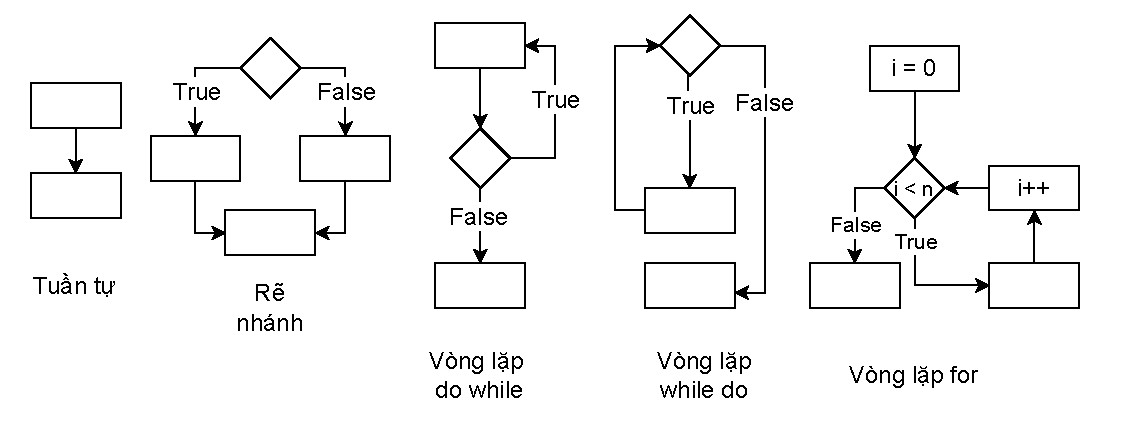
\includegraphics[width=\textwidth]{figures/cfg-control.pdf}
%  		\vspace*{-7mm}
% 		\caption{Các cấu trúc điều khiển phổ biến trong TypeScript}
% 		\label{cau-truc-dieu-khien}
% \end{figure}

% Hình~\ref{cau-truc-dieu-khien} mô tả các cấu trúc điều khiển chính có trong TypeScript được mô phỏng dưới dạng các đỉnh của CFG, bao gồm có cấu trúc điều khiển tuần tự, rẽ nhánh, vòng lặp \textit{for}, vòng lặp \textit{do…while}, vòng lặp \textit{ while…do}.

% \section{Các độ đo kiểm thử}
% Các độ đo kiểm thử thường được xác định là các quy tắc hoặc yêu cầu mà một tập hợp dữ liệu kiểm thử cần đáp ứng \cite{coverage_criteria}. Có một số độ đo phổ biến là bao phủ hàm (function coverage), bao phủ câu lệnh (statement coverage) và bao phủ nhánh (branch coverage). Bao phủ hàm là độ đo dễ đạt được nhất trong ba tiêu chí bao phủ này. Nó được đo bằng tỷ lệ phần trăm các hàm hoặc phương thức đã thực thi trên tổng số các hàm/phương thức có trong mã nguồn thử nghiệm. Bởi vì một hàm được thực thi có thể chứa các đoạn chưa được thực thi như các câu lệnh và các nhánh, một số lỗi bên trong một hàm có thể không được xem xét. Để giải quyết vấn đề này, quá trình kiểm tra phải được thực hiện với cả phạm vi bao phủ của câu lệnh và phạm vi bao phủ nhánh. Liên quan đến bao phủ câu lệnh, nó được biểu thị bằng tỷ lệ phần trăm các câu lệnh được thực thi trong tổng số các câu lệnh thuộc phạm vi kiểm thử. Nếu độ phủ câu lệnh đạt 100\%, thì bao phủ hàm/phương thức cũng đạt đến 100\%. Tuy nhiên, nó không thể xác nhận rằng tất cả các nhánh của điều kiện đều được thực thi. Vì vậy, độ phủ nhánh được đề xuất để đánh giá quá trình thử nghiệm một cách toàn diện hơn. Nó được đo bằng phần trăm các nhánh được thực thi trên tất cả các nhánh thuộc phạm vi kiểm thử. Nếu việc thực thi kiểm thử đạt được bao phủ nhánh tối đa, có thể đảm bảo rằng bao phủ câu lệnh và hàm cũng đạt đến giá trị lớn nhất. Vì vậy, bao phủ nhánh được sử dụng là độ đo cơ bản để đánh giá bộ dữ liệu kiểm thử.

% Công thức tổng quát để tính độ phủ theo các độ đo của $n$ tệp được trình bày trong Công thức \ref{coverage_equation}:
% \begin{equation} \label{coverage_equation}
% \begin{split}
%         e_c &= f(c, tested\ files) \\
%         &= \frac{\sum_{i=1}^n e_{i_c}}
%         {\sum_{i=1}^n t_{i_c}}*100 \\
%  \end{split}
% \end{equation}
% ,trong đó: $c$: loại độ đo bao phủ, bao gồm bao phủ hàm (\textit{function coverage}), bao phủ câu lệnh (\textit{statement coverage}), bao phủ nhánh (\textit{branch coverage})\\
% $e_{i_c}$: số lượng các thành phần được thực thi theo từng độ đo $c$ trong tệp thứ $i$. Thành phần được coi là các hàm, câu lệnh, và nhánh trong mã nguồn kiểm thử. \\
% $t_{i_c}$: số lượng tất cả các thành phần theo độ đo $c$ trong tệp thứ $i$

% Các tiêu chí bao phủ này được sử dụng để đánh giá hiệu quả của phương pháp được đề xuất trong việc tạo dữ liệu thử nghiệm. Nếu độ phủ tăng lên, nhiều thành phần trong mã nguồn được thực thi. Trong trường hợp các độ phủ không đạt 100 \%, các vấn đề sau có thể gặp phải. Thứ nhất, dữ liệu kiểm thử không thực thi toàn bộ các thành phần có trong mã nguồn. Do đó, có thể có một số lỗi tiềm ẩn không được phát hiện. Mặt khác, mã nguồn có thể chứa những câu lệnh không bao giờ có thể thực thi. Các nhà phát triển phải loại bỏ những đoạn mã này để tối ưu kích thước chương trình, tránh thực hiện các hành vi không đúng hoặc đơn giản hóa cấu trúc chương trình.

% % Trong kiểm thử hộp trắng nói chung và kiểm thử dòng điều khiển nói riêng, bài toán kiểm thử là sinh được bộ dữ liệu kiểm thử sao cho thỏa mãn các tiêu chuẩn cho trước. Các tiêu chuẩn này đã được thống nhất và định nghĩa bằng văn bản trong ISO \cite{iso_coverage}. Công thức tính toán độ đo theo các tiêu chuẩn này dựa trên mức độ bao phủ của chương trình với một tập dữ liệu kiểm thử cho trước. Tập dữ liệu kiểm thử có độ phủ cao sẽ đáng tin cậy hơn tập dữ liệu kiểm thử có độ phủ thấp. Mục tiêu là tập dữ liệu kiểm thử có số lượng tối thiểu nhưng đạt được độ phủ tối đa. Hiện nay, có nhiều tiêu chuẩn bao phủ khác nhau được sử dụng. Độ phủ của mỗi tiêu chuẩn đánh giá đều có công thức tính riêng nhưng về cơ bản sẽ được tính bằng tỉ lệ thành phần được kiểm thử trên tổng số các thành phần cần kiểm thử. Thành phần ở đây có thể là câu lệnh, nhánh chương trình, điểm quyết định, điều kiện con hoặc sự kết hợp giữa chúng. Độ đo này giúp các kỹ thuật viên kiểm soát và quản lý quá trình kiểm thử tốt hơn, có thể kiểm tra lại thành phần không được chạy qua hoặc bổ sung thêm dữ liệu kiểm thử trong trường hợp độ phủ thấp. Dưới đây là ba độ đo kiểm thử được sử dụng nhiều trong quy trình kiểm thử phần mềm \cite{Lee03}.
% % \begin{itemize}
% %     \item Độ phủ câu lệnh (statement coverage): mỗi câu lệnh được đi qua ít nhất một lần sau khi chạy bộ dữ liệu kiểm thử.
% %     \item Độ phủ nhánh (branch coverage): nhánh đúng và nhánh sai của mỗi đỉnh điều kiện có trong đồ thị dòng điều khiển được đi qua ít nhất một lần sau khi chạy bộ dữ liệu kiểm thử.
% %     \item Độ phủ điều kiện con (Modified Condition/Decision Coverage - MC/DC): các điều kiện con thuộc các đỉnh điều kiện phức tạp đều được thực hiện cả hai nhánh đúng và nhánh sai ít nhất một lần mỗi nhánh sau khi chạy bộ dữ liệu kiểm thử.
% % \end{itemize}

% % \section{Đường kiểm thử}
% % Bộ dữ liệu kiểm thử sinh ra dành cho một hàm bao gồm nhiều dữ liệu kiểm thử. Mỗi dữ liệu kiểm thử là một bộ giá trị đầu vào của tham số. Với một bộ giá trị đầu vào, chương trình của hàm sẽ chạy qua một số câu lệnh và dừng lại khi tới điểm kết thúc. Tập hợp các câu lệnh theo thứ tự thực hiện tạo thành một đường đi. Những đường đi được chọn để sinh dữ liệu kiểm thử  được gọi là đường kiểm thử. Để thống nhất khái niệm sử dụng trong suốt khóa luận, Định nghĩa 2.4 mô tả tổng quát một đường kiểm thử. Mỗi đường kiểm thử có thể bao gồm đầy đủ các câu lệnh khai báo, gán giá trị, khởi tạo và câu lệnh rẽ nhánh. Các đường đi khác nhau sẽ khác nhau ở số lượng, danh sách và thứ tự thực hiện các câu lệnh. Việc sinh dữ liệu kiểm thử tương ứng với đường kiểm thử chính là tìm kiếm bộ giá trị đầu vào sao cho khi thực thi, các nút điều kiện của đường đi đều được thỏa mãn. Trong thực tế, số lượng đường đi của chương trình có thể rất lớn dẫn đến việc sinh bộ dữ liệu kiểm thử cho tất cả các đường đi là không thể. Vì vậy, một số đường đi được chọn để sinh dữ liệu kiểm thử nhằm đáp ứng tiêu chí về độ phủ được gọi là tập đường kiểm thử.\\
% % \textbf{Định nghĩa 2.1}: Đường kiểm thử là một đường đi từ điểm bắt đầu đến điểm kết thúc của CFG, được biểu diễn bằng tập hợp các đỉnh từ $v_1$  đến $v_n$ sao cho cứ hai đỉnh cạnh nhau thì có cạnh nối theo hướng từ trái qua phải. Nếu cạnh ($v_i$, $v_j$) là nhánh sai thì biểu thức điều kiện tại đỉnh $v_i$ được viết dưới dạng phủ định $!v_i$.

% % Để có thể sinh được bộ dữ liệu kiểm thử thỏa mãn yêu cầu về tiêu chuẩn bao phủ, việc lựa chọn tập kiểm thử là một công đoạn không thể thiếu. Tuy nhiên, có hai vấn đề chúng ta cần phải đối mặt:
% % \vspace{-0.5cm}
% % \begin{itemize}
% %     \item Tính khả thi của đường đi: Một đường kiểm thử gọi là có khả khi nếu tồn tại một dữ liệu kiểm thử sao cho khi thực thi trong môi trường thật, tất cả các đỉnh của đường đi được duyệt qua. Ngược lại, đường kiểm thử gọi là không khả thi.
% %     \item 	Sự bùng nổ đường đi: với một hàm có kích thước lớn, nhiều vòng lặp hoặc các lệnh rẽ nhánh phức tạp, số lượng đường đi của chương trình có thể rất lớn. Việc sinh dữ liệu kiểm thử cho tất cả các đường đi để chắc chắn đạt độ phủ 100\% là không thể.
% % \end{itemize}
% % Mục tiêu của khóa luận này là xây dựng công cụ đầu tiên hỗ trợ sinh dữ liệu kiểm thử cho TypeScript, bắt đầu thử nghiệm với các hàm TypeScript kích thước vừa phải. Vì vậy, tập đường kiểm thử được lựa chọn là tập các đường đi có thể có của chương trình. Trong trường hợp tất cả các đường đi đều khả thi, độ bao phủ nhánh có thể đạt được là 100\%.

% % \section{Thư viện sử dụng}

% % \subsection{Thư viện phân tích mã nguồn TypeScript ``ts-morph''}
% % Phương pháp sinh dữ liệu kiểm thử tự động được đề xuất trong khóa luận này dựa trên việc thao tác với CFG của hàm. Việc xây dựng CFG như thế nào sẽ tùy biến theo từng tình huống bài toán. Đặc biệt đối với một ngôn ngữ mới như TypeScript, hiện tại không có thư viện nào có thể hỗ trợ giải quyết tác vụ này. Vì vậy, quá trình này được thực hiện thủ công dựa trên kỹ thuật phân tích mã nguồn và thiết kế cấu trúc dữ liệu mô hình hóa sao cho phù hợp với bài toán kiểm thử hiện tại. Phân tích mã nguồn thành cây cú pháp trừu tượng (Abstract Syntax Tree - AST) giúp việc xây dựng CFG trở nên đơn giản hơn. AST là một cây đại diện cho cấu trúc cú pháp trừu tượng của mã nguồn. Ngôn ngữ lập trình khác nhau có AST khác nhau.  Mỗi nút của cây biểu thị một cấu trúc có trong mã nguồn. AST thường được xây dựng bởi chính trình phân tích cú pháp của ngôn ngữ tương ứng trong quá trình biên dịch. Đối với các ngôn ngữ lâu đời, việc này có thể được thực hiện bởi một số thư viện khác. Do TypeScript là một ngôn ngữ mới nên chưa có công cụ nào hỗ trợ phân tích mã nguồn thành AST. Vì vậy, khóa luận này sử dụng chính trình biên dịch ngôn ngữ TypeScript của Microsoft để phân tích nội dung hàm. ``ts-morph''\footnote{\url{https://github.com/dsherret/ts-morph}} là một thư viện mở rộng từ trình biên dịch TypeScript, cung cấp các giao diện lập trình ứng dụng (Application Programming Interface - API) hỗ trợ người dùng có một cách dễ dàng hơn để điều hướng chương trình và thao tác với mã TypeScript.
% % Với sự hỗ trợ của ``ts-morph'', người sử dụng có đầy đủ các API để trích xuất thông tin cần thiết từ mã nguồn.  Các khối lệnh của thân hàm và các biểu thức  điều kiện đều có thể dễ dàng có được thông qua việc duyệt các đỉnh, hay gọi là $node$ của AST. Ngoài ra, thư viện cung cấp giao diện\footnote{\url{https://TypeScript-ast-viewer.com/}} để người dùng có thể theo dõi kết quả dưới dạng hình cây rất trực quan và dễ nhìn. Từ đó, việc thao tác với AST trở nên dễ dàng hơn.

% % %  Đối với TypeScript, các cấu trúc này có thể là lớp, hàm, thuộc tính, tham số, câu lệnh, v.v.

% % \subsection{Bộ giải hệ ràng buộc Z3}
% % Công cụ sinh dữ liệu kiểm thử cho mỗi đường kiểm thử bằng cách giải hệ ràng buộc ứng với tập các đỉnh điều kiện. Giải hệ ràng buộc nghĩa là quá trình tìm ra giải pháp cho một tập hợp các ràng buộc áp đặt bởi các phép toán điều kiện mà các biến phải thỏa mãn \cite{ref-constraints}. Do đó, một giải pháp là một tập hợp các giá trị cho các biến thỏa mãn tất cả các ràng buộc, đó là một điểm trong vùng khả thi.
% % Hiện nay, có nhiều thư viện, công cụ hỗ trợ việc giải hệ trong đó nổi bật là bộ giải Z3. Bộ giải Z3 được xây dựng chủ yếu bằng ngôn ngữ C++. Các ràng buộc cần được chuyển sang dạng chuẩn của Z3 để công cụ có thể tính toán và giải nghiệm. Z3 có thể giải hệ ràng buộc của các số nguyên, số thực, mảng và hàm tượng trưng. Đặc biệt trong phiên bản 4.8, bộ giải Z3 hỗ trợ giải một số ràng buộc liên quan đến chuỗi (string) \cite{z3_str_paper}. Điều này giúp việc tìm kiếm dữ liệu kiểm thử có tham số đầu vào kiểu chuỗi trở nên đơn giản hơn. Để có thể sử dụng Z3 giải nghiệm, bộ ràng buộc được lưu trong tệp và khởi chạy tiến trình bằng dòng lệnh:
% % \vspace{0.5cm}
% % \begin{lstlisting}
% % z3 -smt2 <file name>.smt2
% % \end{lstlisting}
% % Mã nguồn~\ref{constraints-file-example} là ví dụ một tệp constraints.smt2 hợp lệ làm đầu vào cho bộ giải Z3. Trong tệp, các biến sử dụng cần được khai báo bằng cú pháp \textit{declare-fun}. Sau đó, lệnh \textit{assert} được sử dụng để thêm các ràng buộc của hệ. Để kiểm tra hệ ràng buộc có nghiệm hay không, lệnh \textit{check-sat} được gọi. Kết quả trả về là \textit{sat} nếu có nghiệm và \textit{unsat} trong trường hợp không có nghiệm. Tập các giá trị của các biến thỏa mãn hệ ràng buộc được hiển thị bằng lệnh \textit{get-model}. Trong ví dụ này, hệ ràng buộc sử dụng ba biến tham số đầu vào là tvw\_s,  tvw\_a, tvw\_b và có ba ràng buộc được thêm vào câu lệnh \textit{assert} trong tệp \textit{constraints.smt2}. Mã nguồn~\ref{z3-result-example} là kết quả tương ứng sau khi giải hệ. Trong đó, các giá trị của các biến tìm được là  tvw\_a = 12,  tvw\_b = 11,  tvw\_s = "\textbackslash x00\textbackslash x00\textbackslash x00\textbackslash x00\textbackslash x00". Như vậy, bộ giá trị (a, b, s) = \{12, 11, "\textbackslash x00\textbackslash x00\textbackslash x00\textbackslash x00\textbackslash x00"\} là một nghiệm của hệ ràng buộc.
% % Nếu áp dụng với một đường kiểm thử cụ thể, các biến được khai báo trong hệ ràng buộc là các biến gọi đến trong các câu lệnh. Các đỉnh điều kiện sẽ được biểu diễn qua những biến này và chuẩn hóa thành những ràng buộc của hệ. Kết quả giải hệ là một dữ liệu kiểm thử thỏa mãn đường đi tương ứng. Trong trường hợp hệ ràng buộc của tất cả các đường đi đều giải được bỏi bộ giải Z3, tập các dữ liệu kiểm thử thu được phủ 100\% đường đi của CFG.

% % \vspace{0.5cm}
% % \begin{lstlisting}[caption=Ví dụ nội dung tệp đầu vào cho bộ giải Z3, label=constraints-file-example,captionpos=b]
% % (set-option :timeout 5000)
% % (declare-fun tvw_s () String)
% % (declare-fun tvw_a () Int)
% % (declare-fun tvw_b () Int)
% % (assert (> a b))
% % (assert (> b 10))
% % (assert (not (> (+ (str.len tvw_s) 1) 10)))
% % (check-sat)
% % (get-model)
% % \end{lstlisting}

% % \begin{lstlisting}[caption=Ví dụ kết quả giải hệ của Z3, label=z3-result-example, captionpos=b]
% % sat
% % (model
% %   (define-fun tvw_s () String
% %     "\x00\x00\x00\x00\x00")
% %   (define-fun tvw_b () Int
% %     11)
% %   (define-fun tvw_a () Int
% %     12)
% % )

% % \end{lstlisting}

% % \subsection{Mocha và Istanbul}
% % Để kiểm tra độ phủ đạt được với bộ dữ liệu kiểm thử đã được sinh tự động, công cụ có sử dụng Mocha trong việc thực thi mã nguồn. Mocha (Mocha Test Framework) là một bộ công cụ hỗ trợ kiểm thử dành cho JavaScript giàu tính năng chạy trên Nodejs và trong trình duyệt, giúp cho việc kiểm tra bất đồng bộ trở nên đơn giản và thú vị \cite{ref-mocha}. Các quy trình thực thi kiểm thử thực hiện bởi Mocha chạy ổn định, cho phép báo cáo linh hoạt và chính xác. Mocha có thể áp dụng với TypeScript thông qua một số bước cài đặt kỹ thuật. Ngoài ra,  Mocha cũng có thể kết hợp với một số thư viện để xuất báo cáo kiểm tra độ phủ (test coverage report). Ngoài việc cung cấp chức năng chạy kiểm thử với thao tác bằng tay, Mocha còn kèm theo bộ API để vận hành các bài kiểm tra tự động. Mocha có rất nhiều tính năng tuyệt vời, trong đó có một số tính năng nổi bật được kể đến là:
% % \begin{itemize}
% %     \item Hỗ trợ bất đồng bộ đơn giản
% %     \item Cung cấp đa dạng báo cáo
% %     \item Có thể chạy trong trình duyệt
% %     \item Tương thích với nhiều thư viện xác nhận (assertion library) Javascript
% %     \item Tương thích với mô hình phát triển phần mềm định hướng hành vi (Behaviour Driven Development - BDD) và mô hình phát triển phần mềm định hướng kiểm thử (Test Driven Development - TDD)
% % \end{itemize}
% % Với sự hỗ trợ của Mocha, các tệp kiểm thử được thực thi một cách nhanh chóng. Kết quả chạy kiểm thử được thống kê trực quan với số lượng dữ liệu kiểm thử thành công hay thất bại kèm theo vị trí cụ thể. Từ đó kỹ thuật viên nhanh chóng xác định được dữ liệu kiểm thử bị sai và dễ dàng sửa chữa.

% % Mocha chỉ hỗ trợ quá trình thực thi tệp kiểm thử và thống kê kết quả số lượng dữ liệu kiểm thử thành công hay thất bại. Tuy nhiên, để có thể biết được thống kê độ phủ mà bộ dữ liệu kiểm thử đạt được, Mocha cần kết hợp thêm một số thư viện bên ngoài. trong đó, được sử dụng nhiều nhất phải kể đến thư viện Istanbul \cite{ref-instanbul}. Đây là thư viện hỗ trợ sinh báo cáo độ phủ của quá trình kiểm thử đơn vị với nhiều định dạng khác nhau như HTML, XML, terminal output, JSON, v.v. Người dùng có thể lựa chọn kiểu báo cáo phù hợp với nhu cầu. Công cụ được phát triển trong khóa luận sử dụng báo cáo thể hiện dưới dạng HTML, bao gồm các thông tin về các độ phủ như số lượng hàm, câu lệnh, nhánh được thực thi. Đồng thời, báo cáo cũng nổi bật các đoạn mã không được chạy qua. Từ đó, kỹ thuật viên có thể phát hiện ra  được các đoạn mã không bao giờ được chạy để làm sạch mã nguồn hoặc bổ sung thêm dữ liệu kiểm thử mới để bộ dữ liệu kiểm thử hoàn thiện hơn.

% \chapter{Phương pháp kiểm thử tự động hàm Typescript sử dụng kỹ thuật kiểm thử tĩnh luồng điểu khiển }
\chapter{LỰA CHỌN VÀ XÂY DỰNG THIẾT BỊ\label{the_proposed_method_section}}

\section{Phần cứng thực nghiệm \label{section_overview_propsed_method}}
\subsection{Cảm biến \label{section_overview_propsed_method}}

Trong quá trình ngủ, các chuyển động thân thể chủ yếu là chuyển động 
chậm, với biên độ nhỏ và không mang tính đột ngột. 
Các chuyển động thân thể chủ yếu mang tính chậm và thường xảy ra 
trong giai đoạn ngủ không chuyển động mắt nhanh (NREM), 
khi cơ thể có khả năng tự do thay đổi tư thế. Ngược lại, 
trong giai đoạn ngủ REM, hiện tượng ức chế trương lực cơ khiến 
cơ thể gần như bất động.
Do đó, việc ghi 
nhận chính xác các thay đổi tư thế ngủ đòi hỏi cảm biến có độ nhạy cao, 
khả năng phân giải tốt và ổn định với nhiễu nền thấp. Như đã trình bày 
trong Chương I, các cảm biến gia tốc MEMS sử dụng nguyên lý điện dung 
hiện đang được ứng dụng rộng rãi trong giám sát tư thế và chuyển động 
khi ngủ nhờ vào đặc điểm nổi bật là kích thước nhỏ gọn, tiêu thụ năng 
lượng thấp, tần số lấy mẫu phù hợp và đặc biệt là độ nhạy cao với 
chuyển động cường độ thấp.

Trong nghiên cứu của Vu và cộng sự (2023), dữ liệu tư thế ngủ được thu 
thập thông qua một thiết bị đeo đặt tại vùng bụng của người tham gia. 
Thiết bị này tích hợp cảm biến gia tốc ba trục ADXL345, 
bộ điều khiển ESP8266 và pin Lithium, tất cả được đóng gói trong 
một hộp nhựa nhỏ gọn \cite{vu2023}. Trong nghiên cứu của Boiko 
và cộng sự, cảm biến gia tốc ba trục ADXL355z 
được sử dụng để thu nhận tín hiệu hô hấp từ vùng ngực và bụng, 
với tần số lấy mẫu 62 Hz. Đây là cảm biến có độ nhiễu thấp, 
độ trôi nhiệt nhỏ và phù hợp với các ứng dụng y sinh. Trước đó, 
dòng cảm biến này cũng đã được ứng dụng thành công trong các phép 
đo tim–phổi \cite{Boiko2023}. Dữ liệu từ ADXL355z được đối chiếu với tín hiệu chuẩn 
thu từ dây đeo hô hấp của hệ thống SOMNO HD eco PSG, nhằm đảm bảo 
độ chính xác trong đánh giá tín hiệu sinh lý trong khi ngủ.
Trong nghiên cứu của Abdulsadig và cộng sự, dữ liệu gia tốc được 
thu thập bằng bo mạch điện tử thiết kế riêng tích hợp cảm biến gia tốc 
ba trục LIS2DH12 (STMicroelectronics) và vi điều khiển nRF5232 
(Nordic Semiconductor) \cite{Sleep_Posture_Detection}.


Dựa trên khảo sát thực tế và đánh giá các tiêu chí kỹ thuật phù hợp 
với đặc thù đo chuyển động chậm khi ngủ, luận văn lựa chọn hai dòng 
cảm biến gia tốc phổ biến là LIS3DH và LSM6DS3, đều do hãng 
STMicroelectronics sản xuất. Cả hai cảm biến đều tích hợp khả năng đo gia tốc ba trục, 
hỗ trợ các chuẩn giao tiếp \texttt{I\textsuperscript{2}C} và \texttt{SPI}, 
đồng thời có thể hoạt động trong chế độ tiêu thụ điện năng siêu thấp (\textit{ultra-low power mode}), 
đáp ứng yêu cầu sử dụng lâu dài trong các thiết bị đeo cá nhân hoạt động liên 
tục suốt đêm.

Trong các ứng dụng theo dõi tư thế ngủ, độ nhạy của cảm biến là một 
trong những tiêu chí quan trọng hàng đầu, bởi nó quyết định khả năng 
phát hiện các chuyển động nhỏ đặc trưng với biên độ thấp và tốc độ 
thay đổi chậm. Cảm biến \textbf{LIS3DH} cho phép lập trình dải đo động 
từ $\pm2g$ đến $\pm16g$, mang lại tính linh hoạt cao trong thiết kế hệ 
thống. Tuy nhiên, khi mở rộng dải đo, độ nhạy và độ phân giải sẽ giảm 
đáng kể. Ví dụ, đối với cảm biến 16-bit, nếu cấu hình ở dải $\pm100g$, 
độ phân giải chỉ đạt khoảng $0{,}003g$/LSB, điều này có thể làm suy giảm 
khả năng nhận biết các chuyển động vi mô trong khi ngủ - một yếu tố 
then chốt trong phân loại chính xác tư thế ngủ.




\begin{figure}[!ht]
		\centering
 		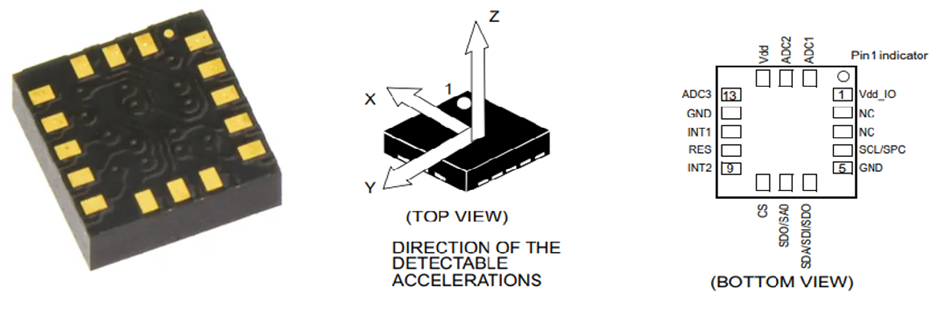
\includegraphics[width=0.8\textwidth]{images/lis.png}
		\caption{Cảm biến gia tốc LIS3DH và sơ đồ chân kết nối}
		\label{lis}
\end{figure}




\subsection{Vi xử lý}

Với sự phát triển vượt bậc và đa dạng của công nghệ chế tạo, 
có rất nhiều cấu hình phần cứng được nhiều nhóm tác giả lựa chọn phù 
hợp với các mục đích khác nhau. Trong đó, \cite{p_1} các tác giả đã 
sử dụng máy tính đơn Raspberry Pi kết hợp các điện trở cảm biến 
lực để phát hiện 4 tư thế ngủ với sự lấy nhãn từ video theo dõi người 
bệnh trong suốt quá trình lấy mẫu. Kwasnicki và cộng sự đã phát triển 
hệ thống ngủ có thể đeo (wearable sleep system) sử dụng bộ xử lý công 
suất thấp TI MSP430 và mô-đun RF Chipcon CC2420 cho truyền thông không 
dây kết hợp với cảm biến gia tốc 3 trục ADXL330, con quay hồi chuyển 
InvenSense ITG-3200, Honeywell HMC5843 để đo từ trường xác định 99.5\% 
chính xác 4 tư thế ngủ \cite{kwasnicki2018}. Tuy nhiên, các thiết bị vẫn 
yêu cầu một nguồn nặng lượng khiến cho tính liên tục bị hạn chế đáng kể. 
I.Yun và cộng sự đã phát triển thiết bị theo dõi tư thế ngủ của trẻ nhỏ 
sử dụng vi xử lý ATmega328P-PU cùng module Bluetooth kết hợp cảm biến gia 
tốc ADXL335 được đặt trên bụng đã nhưng lựa chọn về mặt cấu hình thiết bị 
và chế tạo ra mạch cung cấp năng lượng cho những thành phần cần thiết 
\cite{p_3}. Từ đó, giảm thiếu đáng kể mức tiêu thụ năng lượng và vẫn 
giữ nguyên độ chính xác nhưng khá bất tiện cho trẻ nhỏ. 
Trong nghiên cứu của Abdulsadig và cộng sự, 
hệ thống thu thập dữ liệu được xây dựng dựa trên một bo mạch tùy chỉnh tích 
hợp vi điều khiển nRF5232 (Nordic Semiconductor) – một SoC thuộc dòng 
ARM Cortex-M4F, hỗ trợ truyền thông không dây thông qua giao 
thức Bluetooth Low Energy (BLE). Vi điều khiển này đảm nhiệm đồng 
thời cả việc lấy mẫu dữ liệu từ cảm biến gia tốc ba trục LIS2DH12 
(STMicroelectronics) với tần số 100 Hz và truyền dữ liệu không dây 
theo thời gian thực \cite{Sleep_Posture_Detection, abdulsadig2023}. 
Trong nghiên cứu của Vũ Hoàng Diệu và cộng sự, 
mô-đun ESP32 được lựa chọn làm đơn vị xử lý trung tâm nhờ tích hợp bộ vi điều khiển hiệu năng cao, 
kết nối không dây Wi-Fi và khả năng mở rộng linh hoạt \cite{vu2023}. 
Với thiết kế nhỏ gọn, chi phí hợp lý và mức tiêu thụ điện năng thấp, 
ESP32 đáp ứng tốt yêu cầu của hệ thống thu thập dữ liệu tư thế ngủ theo 
thời gian thực. Thiết bị không chỉ cho phép truyền dữ liệu trực tiếp 
lên máy chủ hoặc nền tảng đám mây thông qua Wi-Fi, mà còn hỗ trợ 
lưu trữ cục bộ trên thẻ nhớ microSD, đảm bảo tính liên tục và 
an toàn dữ liệu trong điều kiện mất kết nối mạng.

Tuy nhiên, qua phân tích các nghiên cứu trên có thể thấy rằng phần 
lớn các cấu hình phần cứng hiện tại hoặc có chi phí triển khai cao, 
hoặc tiêu tốn năng lượng, hoặc gặp giới hạn trong khả năng tích hợp mô 
hình học máy tại thiết bị. Do đó, việc lựa chọn một kiến trúc vi xử lý 
vừa đảm bảo hiệu suất xử lý tín hiệu sinh lý thời gian thực, vừa tối 
ưu năng lượng và có khả năng triển khai mô hình TinyML là cần thiết. 
Trong số các kiến trúc hiện nay, dòng ARM Cortex-M4 nổi bật nhờ tính 
cân bằng giữa hiệu năng, mức tiêu thụ năng lượng thấp và khả năng hỗ 
trợ xử lý tín hiệu số, phù hợp với các hệ thống đeo được trong theo 
dõi tư thế ngủ.


Kiến trúc ARM có nhiều dòng vi xử lý khác nhau, được phát triển và nâng
cấp liên tục nhằm đáp ứng nhu cầu đa dạng trong lĩnh vực công nghệ nhúng. 
Trong đó, dòng Cortex-M thuộc kiến trúc ARMv7 đã trở thành nền tảng phổ 
biến cho các hệ thống nhúng sử dụng vi điều khiển nhờ vào hiệu suất cao, 
khả năng mở rộng và mức tiêu thụ năng lượng tối ưu. Dòng Cortex-M bao 
gồm nhiều phiên bản như Cortex-M0, Cortex-M0+, Cortex-M1, Cortex-M3, 
Cortex-M4 và Cortex-M7, mỗi phiên bản được thiết kế để phục vụ cho các mức 
độ yêu cầu hiệu năng khác nhau \cite{arm_cortex_m_comparison}. 
Các vi xử lý thuộc họ Cortex-M chủ yếu được ứng dụng trong các hệ thống 
nhúng thời gian thực, nơi yêu cầu sự cân bằng giữa hiệu suất xử lý, tiêu 
thụ năng lượng và chi phí. Một số vi xử lý ARM khác, không thuộc họ 
Cortex-M, được sử dụng trong các thiết bị hiệu suất cao như điện thoại 
thông minh và máy tính bảng, vốn yêu cầu cấu hình phần cứng mạnh hơn và 
khả năng xử lý đa tác vụ cao hơn.
Theo tài liệu \cite{cortexM4}, vi xử lý Cortex-M4 là một bộ xử lý 32-bit 
sử dụng kiến trúc tập lệnh rút gọn (RISC), được xây dựng theo kiến trúc 
Harvard, trong đó bus dữ liệu và bus lệnh được tách biệt nhằm tối ưu 
hiệu suất truy xuất bộ nhớ. Vi xử lý này hỗ trợ đầy đủ cả tập lệnh 
Thumb-1 (16-bit) và Thumb-2 (hỗn hợp 16/32-bit), mang lại sự linh hoạt 
trong mã hóa lệnh và tiết kiệm không gian bộ nhớ chương trình.

Về hiệu năng, Cortex-M4 đạt từ 1,25 đến 1,95 DMIPS/MHz (Dhrystone Million Instructions Per Second per MHz), cho thấy khả năng xử lý hiệu quả trong các ứng dụng nhúng yêu cầu độ chính xác và độ phản hồi thời gian thực cao. Bên cạnh đó, vi xử lý hỗ trợ tối đa 240 tín hiệu ngắt, bao gồm cả ngắt không thể bị chặn (Non-Maskable Interrupts – NMI), cùng khả năng cấu hình từ 8 đến 256 mức ưu tiên ngắt, giúp hệ thống hoạt động ổn định trong môi trường có nhiều sự kiện cạnh tranh đồng thời.
Ngoài ra, hiện nay ứng dụng trí tuệ nhân tạo (AI) tại thiết bị biên (Edge AI) đang ngày càng phổ biến, đặc biệt trong các lĩnh vực như nhà thông minh, thiết bị đeo, giám sát an ninh và công nghiệp 4.0. Với khả năng xử lý tín hiệu số (DSP) và hỗ trợ các mạng nơ-ron nhỏ gọn, các vi xử lý Cortex-M, đặc biệt là dòng Cortex-M4, đang được khai thác để triển khai các mô hình học sâu nhẹ (tinyML) ngay trên vi điều khiển \cite{electronics11162545}\cite{applicationCortexM4}.


\begin{figure}[!ht]
		\centering
 		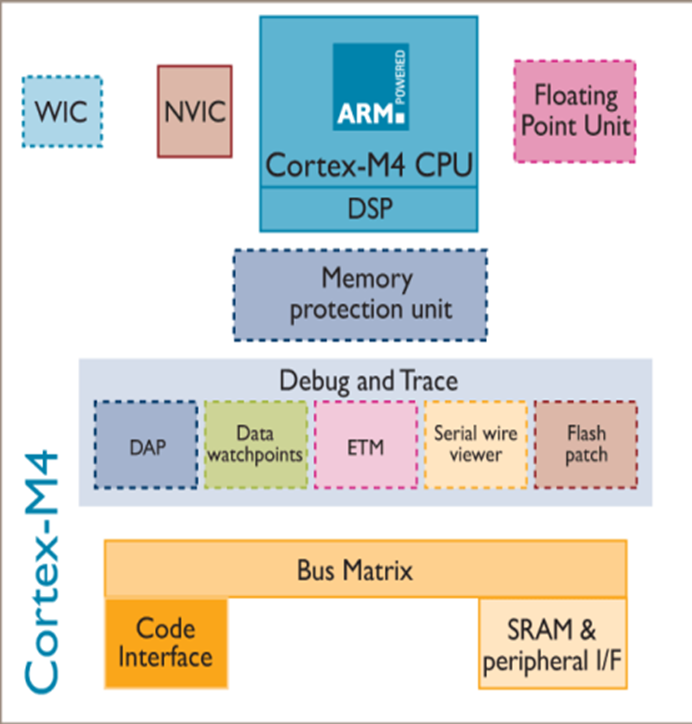
\includegraphics[width=0.8\textwidth]{images/cortexM4.png}
		\caption{Thành phần chính của vi điều khiển Cortex-M4}
		\label{cortexM4}
\end{figure}

Kết nối bus được mô tả trong Hình~\ref{cortexM4} cho phép truyền dữ liệu đồng thời trên nhiều bus khác nhau, đồng thời cung cấp khả năng quản lý truyền dữ liệu hiệu quả, chẳng hạn như sử dụng bộ đệm ghi và điều khiển hướng bit hoạt động (bit-banding). Hệ thống cũng có thể bao gồm các cầu bus (bus bridges) nhằm kết nối nhiều loại bus vào một mạng duy nhất sử dụng chung không gian bộ nhớ. Ngoài ra, bộ xử lý được trang bị hệ thống hỗ trợ gỡ lỗi tích hợp, bao gồm khả năng kiểm soát gỡ lỗi, thiết lập điểm ngắt (breakpoint) chương trình và điểm theo dõi dữ liệu (watchpoint). Khi xảy ra sự kiện gỡ lỗi, hệ thống có thể tạm dừng trạng thái hoạt động của lõi xử lý để phục vụ việc phân tích và xử lý lỗi.

Bên cạnh đó, kiến trúc Cortex-M4 tích hợp Bộ điều khiển ngắt vectored lồng nhau (Nested Vectored Interrupt Controller – NVIC) với khả năng hỗ trợ lên đến 240 tín hiệu yêu cầu ngắt, bao gồm cả ngắt không chắn được (NMI). NVIC hỗ trợ xử lý ngắt lồng nhau một cách tự động bằng cách so sánh mức ưu tiên giữa các yêu cầu ngắt với mức ưu tiên hiện tại đang được xử lý.

Đối với các ứng dụng yêu cầu tiết kiệm năng lượng, hệ thống còn được trang bị bộ đánh thức ngắt (Wake-up Interrupt Controller – WIC), cho phép đưa bộ vi điều khiển vào chế độ nghỉ bằng cách tắt hầu hết các thành phần không cần thiết, đồng thời duy trì khả năng đánh thức hệ thống khi phát hiện một yêu cầu ngắt. Ngoài ra, cơ chế bảo vệ bộ nhớ cũng được tích hợp nhằm đảm bảo an toàn cho hệ thống, ví dụ như chỉ cho phép truy cập đọc tại một số vùng bộ nhớ hoặc ngăn người dùng truy cập vào các vùng dữ liệu đặc quyền của hệ điều hành hoặc ứng dụng hệ thống.


\begin{figure}[!ht]
		\centering
 		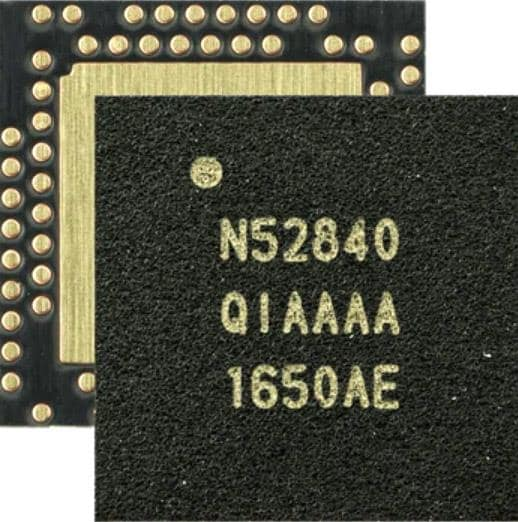
\includegraphics[width=0.8\textwidth]{images/NRF52840-QFA_SPL.jpg}
		\caption{Nordic Semiconductor NRF52840}
		\label{lis}
\end{figure}
Sau quá trình khảo sát và so sánh các dòng vi xử lý phổ biến, tác giả 
lựa chọn nRF52840 (Nordic Semiconductor) làm nền tảng phần cứng cho hệ 
thống đề xuất, nhờ vào các ưu điểm nổi bật như kích thước nhỏ, 
tiêu thụ năng lượng thấp và tích hợp sẵn giao tiếp Bluetooth Low Energy 
(BLE). Đây là vi xử lý cao cấp nhất trong dòng nRF52, thuộc loại hệ thống 
trên một vi mạch (System-on-Chip – SoC), được thiết kế chuyên biệt cho 
các ứng dụng không dây tầm ngắn và tiết kiệm năng lượng \cite{nrf52840}.

\textbf{nRF52840} tích hợp bộ thu phát đa giao thức hoạt động ở băng tần 2.4 GHz 
và bộ xử lý trung tâm Arm Cortex-M4F chạy ở xung nhịp 64 MHz, 
kèm bộ xử lý dấu phẩy động (FPU). Vi xử lý này được trang bị bộ nhớ 
1 MB Flash và 256 KB RAM, hỗ trợ chuẩn Bluetooth 5.3 cùng khả năng giao 
tiếp đa giao thức (multiprotocol), cho phép cải thiện tốc độ, phạm vi 
truyền và độ tin cậy của kết nối không dây. Hệ thống bảo mật tích hợp 
đầy đủ, bao gồm các tính năng mã hóa phần cứng, đáp ứng yêu cầu khắt khe 
về bảo vệ dữ liệu. Ngoài khả năng hoạt động trong dải điện áp rộng 
từ +1.7 V đến +5.5 V (tương thích với nguồn pin và USB), nRF52840 còn 
cung cấp các giao tiếp ngoại vi phong phú: tối đa hai giao diện I2C, 
bốn SPI master, ba SPI slave, bốn kênh PWM hỗ trợ EasyDMA, cùng với 
năm bộ định thời 32-bit, phù hợp cho các ứng dụng đòi hỏi xử lý thời 
gian thực chính xác. Tất cả các đặc điểm trên khiến nRF52840 trở thành 
lựa chọn lý tưởng cho các hệ thống nhúng đeo được tích hợp AI nhẹ và 
kết nối không dây thông minh.

Ngoài ra, nRF52840 hỗ trợ một hệ sinh thái phần mềm mạnh mẽ, bao gồm SDK 
của Nordic và nền tảng TensorFlow Lite for Microcontrollers, giúp rút 
ngắn thời gian phát triển và triển khai hệ thống TinyML. Thiết bị còn 
sở hữu khả năng quản lý năng lượng linh hoạt, tương thích tốt với nguồn pin hoặc USB. 





\subsection{Bluetooth năng lượng thấp}

Với mục tiêu tối ưu hóa năng lượng và đảm bảo khả năng hoạt động lâu dài 
cho thiết bị đeo sử dụng pin, Bluetooth Low Energy (BLE) được lựa chọn 
làm chuẩn kết nối không dây chính trong hệ thống phần cứng.

\begin{figure}[!ht]
		\centering
 		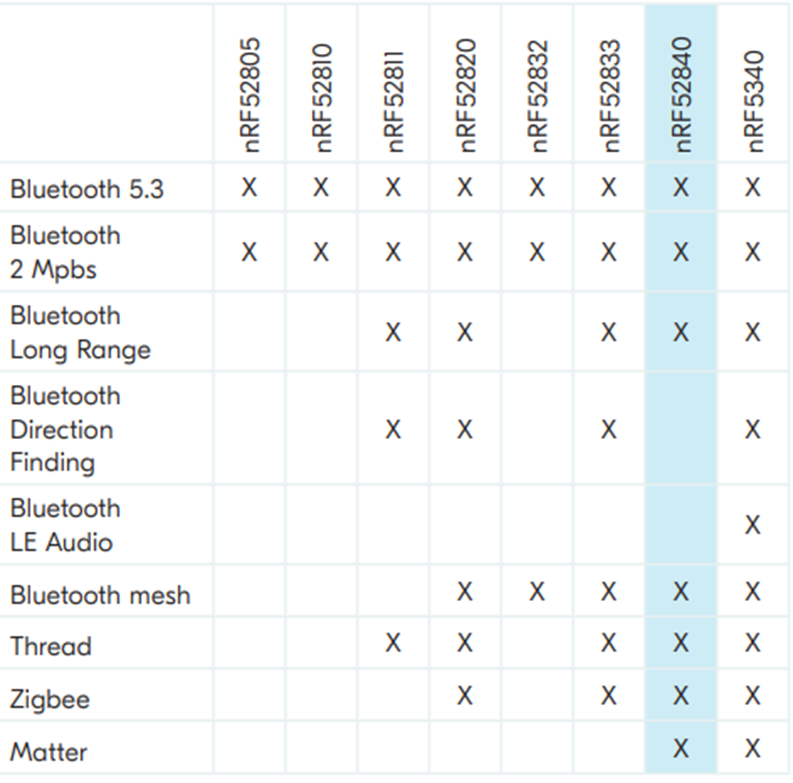
\includegraphics[width=0.8\textwidth]{images/ble.png}
		\caption{Các kiểu kết nối không dây trong họ chip nRF52}
		\label{ble}
\end{figure}

BLE là giao thức kết nối không dây được thiết kế chuyên biệt cho 
các ứng dụng năng lượng thấp, hoạt động ở băng tần ISM 2.4 GHz, 
hỗ trợ thông lượng ứng dụng lên đến 1.4 Mbps. Với ưu thế tiêu thụ năng 
lượng tối thiểu nhưng vẫn đảm bảo tốc độ truyền phù hợp, BLE đặc biệt 
thích hợp cho các thiết bị y sinh hoạt động liên tục bằng pin có dung 
lượng hạn chế. BLE hiện được hỗ trợ phổ biến trên hầu hết các hệ điều 
hành như iOS, Android, macOS, Windows 10 và Linux, cũng như trong các 
thiết bị di động hiện đại.

Về mặt bảo mật, BLE tích hợp các cơ chế mã hóa và xác thực nhằm đảm bảo 
tính bí mật, toàn vẹn và riêng tư của dữ liệu truyền qua mạng. 
Công nghệ này đã trở thành một phần tiêu chuẩn trong hầu hết các 
thiết bị di động hiện đại như smartphone, máy tính bảng, và laptop, 
đồng thời được hỗ trợ đầy đủ trên các hệ điều hành phổ biến bao gồm iOS, 
Android, macOS, Windows 10 và Linux. Bluetooth 5 là bước phát triển 
đột phá tiếp theo kể từ khi BLE được giới thiệu trong chuẩn Bluetooth 
4.0, mang đến hàng loạt cải tiến đáng kể giúp mở rộng phạm vi ứng dụng 
và nâng cao hiệu suất hệ thống. Một trong những cải tiến nổi bật là 
chế độ 2 Mbps, cho phép tăng gấp đôi tốc độ truyền lý thuyết, tương 
ứng với thông lượng thực tế lên đến 1.4 Mbps. Quan trọng hơn, chế độ 
này còn giúp giảm đáng kể mức tiêu thụ năng lượng – cụ thể là giảm một 
nửa năng lượng tiêu thụ trên mỗi bit dữ liệu – từ đó kéo dài thời gian 
hoạt động của thiết bị hoặc cho phép sử dụng các nguồn năng lượng nhỏ 
và chi phí thấp hơn \cite{BLE}. 

Bên cạnh đó, tính năng Advertising Extensions (mở rộng quảng cáo) đã 
cách mạng hóa cơ chế phát sóng của BLE. Các gói quảng cáo giờ đây có 
thể chứa lượng dữ liệu gấp 8 lần so với phiên bản trước, cho phép 
truyền tải các khối dữ liệu lớn hơn mà không cần thiết lập kết nối 
ngay lập tức. Đồng thời, các gói quảng cáo có thể được xâu chuỗi 
để tạo thành các tập tin quảng cáo phức hợp. Tính năng lựa chọn kênh 
được tối ưu hóa giúp tăng cường độ ổn định và khả năng chống nhiễu 
trong các môi trường có mật độ thiết bị cao. Đặc biệt, chế độ Long 
Range mở rộng đáng kể phạm vi truyền thông của BLE, cho phép các thiết 
bị duy trì kết nối trong toàn bộ không gian của một ngôi nhà thông minh 
hoặc trong các ứng dụng IoT công nghiệp quy mô vừa và nhỏ.




\begin{figure}[!ht]
	\centering
 	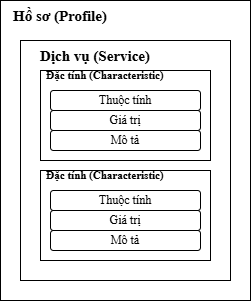
\includegraphics[width=0.5\textwidth]{images/gatt.drawio.png}
	\caption{Cấu trúc của GATT}
	\label{gatt}
\end{figure}

BLE tổ chức logic giao tiếp dựa trên mô hình GATT 
(Generic Attribute Profile). GATT quy định cách hai thiết bị BLE 
trao đổi dữ liệu thông qua các đơn vị logic: dịch vụ (services) 
và đặc tính (characteristics). Giao thức nền tảng là Attribute Protocol 
(ATT) – nơi mỗi đặc tính được định danh bằng UUID 16-bit hoặc 128-bit, 
với quyền truy cập như chỉ đọc, chỉ ghi, hoặc hỗ trợ thông báo (notify).

Một điểm quan trọng trong mô hình GATT là tính kết nối độc quyền: 
tại một thời điểm, thiết bị ngoại vi chỉ có thể duy trì một kết nối 
duy nhất với thiết bị trung tâm. Khi kết nối được thiết lập, thiết bị 
ngừng quảng cáo, điều này hạn chế khả năng kết nối đồng thời từ 
nhiều thiết bị.

Ngoài ra, vi xử lý nRF52840 còn hỗ trợ Bluetooth Mesh, cho phép thiết 
lập mạng lưới nhiều-nút (many-to-many), sử dụng BLE làm lớp truyền tải 
vật lý. Mỗi nút trong mạng có thể đóng vai trò chuyển tiếp (relay), 
cho phép dữ liệu lan truyền đến các vùng rộng hơn theo mô hình phân 
tán – phù hợp với các ứng dụng IoT quy mô lớn như nhà thông minh, 
chiếu sáng công nghiệp hoặc giám sát phân tán. Trong mạng Mesh, 
các gói dữ liệu có thể được đóng gói qua advertising packet hoặc 
qua các giao tiếp GATT tùy tình huống sử dụng.

Các profile BLE là tập hợp các dịch vụ được chuẩn hóa bởi Bluetooth 
SIG hoặc định nghĩa tùy chỉnh, ví dụ như dịch vụ UART tùy chỉnh gồm 
hai đặc tính RX và TX, tương ứng với kênh nhận và truyền.

\subsection{Thiết bị thực nghiệm}
Trong khuôn khổ của khóa luận, nhằm đảm bảo tiến độ triển khai và tính an 
toàn trong giai đoạn thử nghiệm, tác giả lựa chọn sử dụng bộ kit thương 
mại Adafruit Playground để tiến hành thực nghiệm sơ bộ. Bộ kit này tích 
hợp sẵn cảm biến gia tốc MEMS LIS3DH được gắn tại vị trí trung tâm, 
cho phép đo gia tốc theo ba trục không gian X, Y và Z với độ chính xác cao. 
Theo tài liệu từ nhà sản xuất, chi phí cho mỗi bộ kit Adafruit vào khoảng 
25 USD \cite{ada_overview}. Trong bộ kit, cảm biến LIS3DH được kết nối với 
vi điều khiển thông qua giao thức SPI, với chân chọn thiết bị (CS) được 
gán tại chân số 8 và đầu ra ngắt tùy chọn (IRQ) tại chân số 7 (IRQ \#4). 
Theo sơ đồ bố trí tiêu chuẩn của kit, trục X định hướng theo chiều giắc 
USB, trục Y hướng sang bên trái, và trục Z vuông góc theo hướng mặt trên 
của thiết bị.

Bên cạnh đó, để mở rộng khả năng nghiên cứu và đánh giá tính khả thi khi 
tích hợp học máy nhẹ (TinyML) cũng như kết nối không dây, nhóm nghiên 
cứu sử dụng thêm nền tảng Arduino Nano 33 BLE Sense. Đây là vi điều khiển 
hiện đại tích hợp vi xử lý nRF52840 (ARM Cortex-M4F), hỗ trợ Bluetooth 
Low Energy (BLE) và nhiều cảm biến tích hợp (IMU, microphone, nhiệt độ, 
độ ẩm, v.v.), đồng thời tương thích với nền tảng TensorFlow Lite for 
Microcontrollers \cite{nano33ble}.

Đáng chú ý, bên cạnh việc sử dụng các bộ kit sẵn có, một thành viên khác 
trong nhóm đang tiến hành phát triển và xây dựng bản mạch phần cứng 
tùy chỉnh dựa trên các thông số kỹ thuật đã được phân tích ở các phần 
trước. Hướng tiếp cận này không chỉ giúp nhóm triển khai nhanh chóng hệ 
thống thử nghiệm trong giai đoạn đầu, mà còn mở ra khả năng thiết kế một 
thiết bị nhúng chuyên dụng, tối ưu hơn về chi phí, hiệu năng và khả năng 
tích hợp trong các ứng dụng thực tiễn.


\begin{figure}[!ht]
		\centering
 		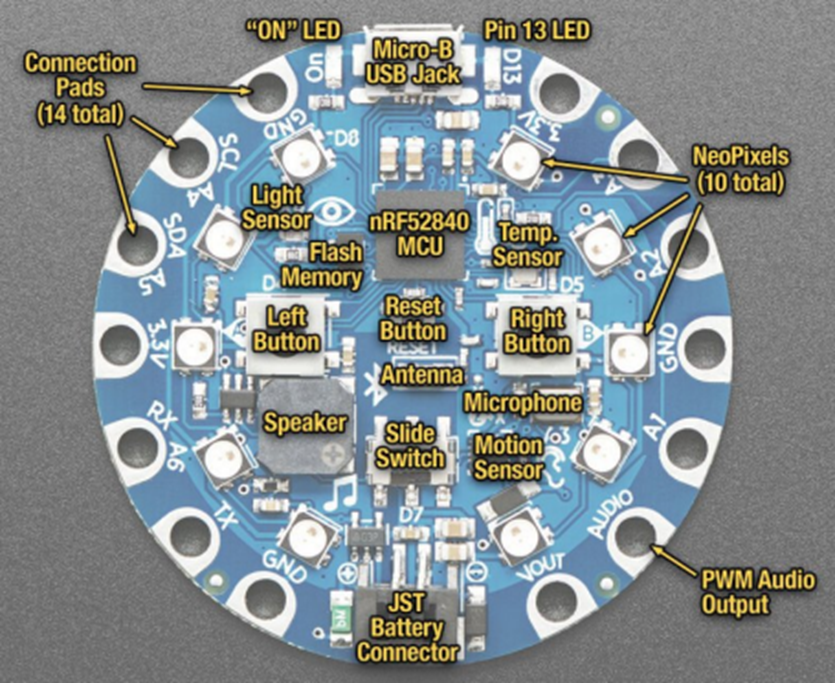
\includegraphics[width=0.8\textwidth]{images/detail_ada.png}
		\caption{Cấu trúc các thành phần trên Circuit PlayGround}
		\label{detail_ada}
\end{figure}





\section{Hệ thống thu thập, xử lý, lưu trữ dữ liệu}
Phần này trình bày tổng quan kiến trúc hệ thống bao gồm: 
lập trình firmware trên vi điều khiển để thu thập dữ liệu cảm biến, 
thiết kế ứng dụng di động làm cầu nối giữa phần cứng và hệ thống đám mây, 
cùng với backend và cơ sở dữ liệu lưu trữ phục vụ huấn luyện mô hình. 
Nội dung cũng đề cập đến các yêu cầu chức năng, phi chức năng và 
thiết kế hệ thống ở mức cao nhằm đảm bảo khả năng triển khai thực 
tế và mở rộng trong tương lai.


\subsection{Lập trình vi xử lý}

Thiết bị được lập trình trên nền tảng Arduino IDE, sử dụng thư viện 
\texttt{Adafruit Circuit Playground}. Trong hàm \texttt{setup()}, 
thiết bị khởi tạo các bản tin quảng cáo (advertising), 
cấu hình kết nối/ngắt kết nối, và thiết lập cấu trúc dịch vụ theo 
giao thức \gls{GATT} của BLE, như được minh họa trong Hình~\ref{flowBLE}.

\begin{figure}[htbp]
    \centering
    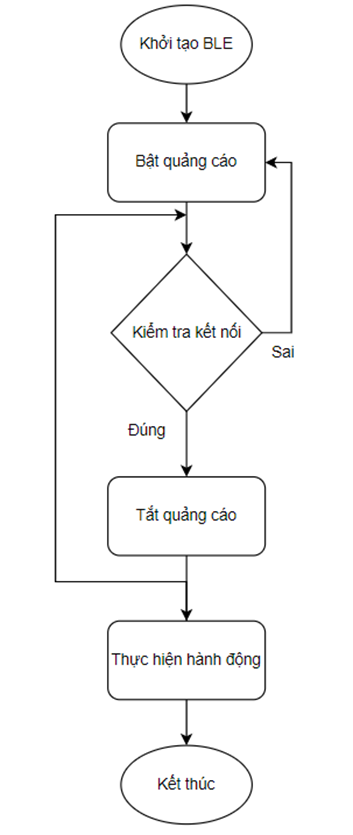
\includegraphics[width=0.5\textwidth]{images/flowBLE.png}
    \caption{Lưu đồ hoạt động của thiết bị BLE}
    \label{flowBLE}
\end{figure}

Trong đoạn mã~\ref{arduinoBLE}, hàm \texttt{startAdv()} đảm nhiệm cấu 
hình quảng bá BLE cho thiết bị. Quá trình này bao gồm: thiết lập cờ 
kết nối tổng quát, chèn thông tin công suất truyền (Tx Power), 
thêm UUID của dịch vụ tư thế (\texttt{positionService}) và tên thiết 
bị vào gói quảng bá. Các thông số quảng bá được cấu hình theo khuyến 
nghị của Apple nhằm đảm bảo khả năng tương thích với thiết bị iOS: 
chế độ nhanh với chu kỳ 20ms, chế độ chậm 152.5ms, và thời gian chuyển 
chế độ sau 30 giây. Thiết bị sẽ tiếp tục phát tín hiệu quảng bá cho 
đến khi có kết nối được thiết lập.

Trong cấu trúc dịch vụ, tác giả định nghĩa một dịch vụ chính với UUID 
là \texttt{0x1821}, kèm theo hai đặc tính cảm biến: gia tốc 
(\texttt{UUID 0x2713}, đơn vị \texttt{m/s\textsuperscript{2}}) và 
gia tốc góc (\texttt{UUID 0x2744}, 
đơn vị \texttt{rad/s\textsuperscript{2}}). 
Tuy hệ thống hỗ trợ cả hai loại dữ liệu, trong khuôn khổ khoá luận này, 
tác giả chỉ tập trung vào giá trị gia tốc thu được từ cảm biến để phục 
vụ bài toán phân loại tư thế ngủ.

\begin{lstlisting}[float,language=C,caption=Tập lệnh khởi tạo và kết nối Bluetooth từ thư viện của AdaFruit, label=arduinoBLE,captionpos=b]
void startAdv(void)
{
  // Advertising packet
  Bluefruit.Advertising.addFlags(BLE_GAP_ADV_FLAGS_LE_ONLY_GENERAL_DISC_MODE);
  Bluefruit.Advertising.addTxPower();

  // Include HRM Service UUID
  Bluefruit.Advertising.addService(positionService);

  // Include Name
  Bluefruit.Advertising.addName();
  
  /* Start Advertising
   * - Enable auto advertising if disconnected
   * - Interval:  fast mode = 20 ms, slow mode = 152.5 ms
   * - Timeout for fast mode is 30 seconds
   * - Start(timeout) with timeout = 0 will advertise forever (until connected)
   * 
   * For recommended advertising interval
   * https://developer.apple.com/library/content/qa/qa1931/_index.html   
   */
  Bluefruit.Advertising.restartOnDisconnect(true);
  Bluefruit.Advertising.setInterval(32, 244);    // in unit of 0.625 ms
  Bluefruit.Advertising.setFastTimeout(30);      // number of seconds in fast mode
  Bluefruit.Advertising.start(0);                // 0 = Don't stop advertising after n seconds  
}
\end{lstlisting}


\begin{lstlisting}[float,language=C,caption=Gửi dữ liệu từ BLE, label=sendBle,captionpos=b]
void setupPosition(void)
{
 
  positionService.begin();

  accelerometerCharacter.setProperties(CHR_PROPS_NOTIFY+CHR_PROPS_READ+CHR_PROPS_WRITE );
  accelerometerCharacter.setPermission(SECMODE_OPEN, SECMODE_NO_ACCESS);
  accelerometerCharacter.setFixedLen(9);
  accelerometerCharacter.setCccdWriteCallback(cccd_callback);  // Optionally capture CCCD updates
  accelerometerCharacter.begin();
  uint8_t accelerometerData[9] = { 0b00000000, 0b00000000, 0b00000000,0b00000000,0b00000000,0b00000000,0b00000000,0b00000000,0b00000000}; // Set the characteristic to use 8-bit values, with the sensor connected and detected
  accelerometerCharacter.write(accelerometerData, 9);

  gyroscopeCharacter.setProperties(CHR_PROPS_READ);
  gyroscopeCharacter.setPermission(SECMODE_OPEN, SECMODE_NO_ACCESS);
  gyroscopeCharacter.setFixedLen(1);
  gyroscopeCharacter.begin();
  gyroscopeCharacter.write8(2);    // Set the characteristic to 'Wrist' (2)
}

\end{lstlisting}

Ngoài các thao tác khởi tạo dịch vụ, thư viện BLE của Adafruit còn cung cấp các phương thức cấu hình đặc tính (\textit{characteristics}) nhằm kiểm soát hành vi và bảo mật của kết nối BLE.

Cụ thể, phương thức \texttt{setProperties} cho phép cấu hình quyền truy cập của đặc tính, với các lựa chọn phổ biến như:

\begin{description}
    \item[\texttt{CHR\_PROPS\_BROADCAST}] phát sóng đặc tính (bit 0)
    \item[\texttt{CHR\_PROPS\_READ}] cho phép thiết bị đọc (bit 1)
    \item[\texttt{CHR\_PROPS\_WRITE\_WO\_RESP}] ghi không cần phản hồi (bit 2)
    \item[\texttt{CHR\_PROPS\_WRITE}] ghi với phản hồi (bit 3)
    \item[\texttt{CHR\_PROPS\_NOTIFY}] gửi thông báo không xác nhận (bit 4)
    \item[\texttt{CHR\_PROPS\_INDICATE}] gửi thông báo có xác nhận (bit 5)
\end{description}

Ngoài ra, một số phương thức bổ trợ khác bao gồm:

\begin{description}
    \item[\texttt{setPermission}] thiết lập quyền truy cập và mức độ bảo mật (ví dụ: không cần xác thực, cần mã hoá, v.v.)
    \item[\texttt{setFixedLen}] xác định độ dài cố định của dữ liệu truyền
\end{description}

\begin{figure}[htbp]
    \centering
    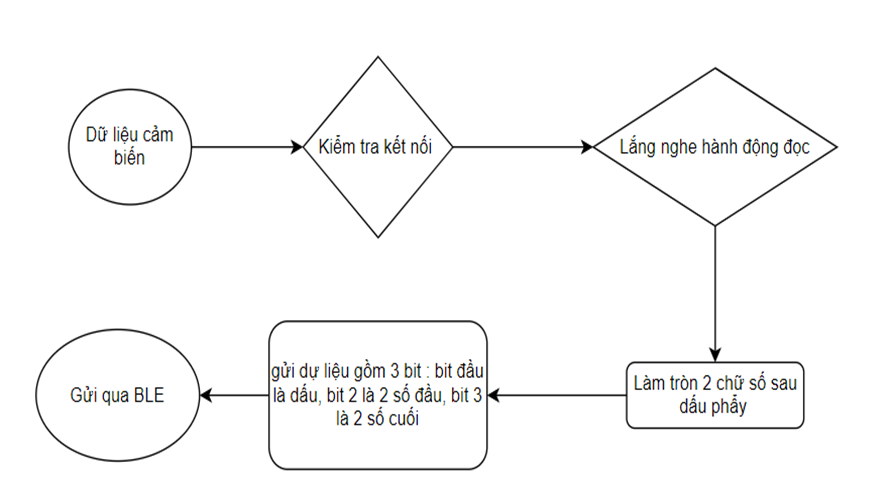
\includegraphics[width=\textwidth]{images/sendBleFlow.png}
    \caption{Lưu đồ luồng gửi thông tin BLE}
    \label{sendBleFlow}
\end{figure}


Luồng xử lý dữ liệu BLE được minh hoạ tại Hình~\ref{sendBleFlow}. 
Sau khi thu nhận dữ liệu cảm biến, thiết bị kiểm tra trạng thái 
kết nối BLE. Nếu kết nối hợp lệ, nó sẽ tiếp tục lắng nghe hành động đọc 
từ phía thiết bị trung tâm. Dữ liệu sau đó được làm tròn đến hai chữ số 
thập phân và mã hoá thành ba byte: byte đầu tiên lưu dấu, byte thứ hai 
chứa hai chữ số đầu, và byte cuối là hai chữ số cuối của giá trị gia tốc. 
Chuỗi dữ liệu này được gửi qua BLE theo đặc tính đã định nghĩa trước đó.














\subsection{Hiệu chuẩn cảm biến}
Việc thu nhận và tiền xử lý dữ liệu là bước quan trọng trong các hệ đo 
lường. Mặc dù cảm biến thường được hiệu chuẩn từ nhà sản xuất, nhưng 
vẫn cần được hiệu chuẩn lại trong môi trường đo thực tế để cải thiện 
hiệu năng và giảm thiểu sai số. Các sai số này được chia thành hai 
loại chính: (i) sai số hệ thống (mặc định) và (ii) sai số ngẫu nhiên.

\textbf{Hiệu chuẩn sai số hệ thống.} Tác giả sử dụng gia tốc trọng trường 
để hiệu chuẩn cảm biến theo hướng tĩnh. Khi xoay cảm biến sao cho một 
trục hướng lên vuông góc với mặt phẳng nằm ngang, giá trị đo được 
là $-1g$; khi hướng xuống dưới, giá trị là $+1g$. Bằng cách xoay cảm 
biến lần lượt qua sáu vị trí tĩnh tương ứng với các hướng trục chính, 
có thể xác định được các điểm chuẩn, từ đó nội suy để xác định giá 
trị $0g$ một cách chính xác và đáng tin cậy.

\begin{figure}[htbp]
    \centering
    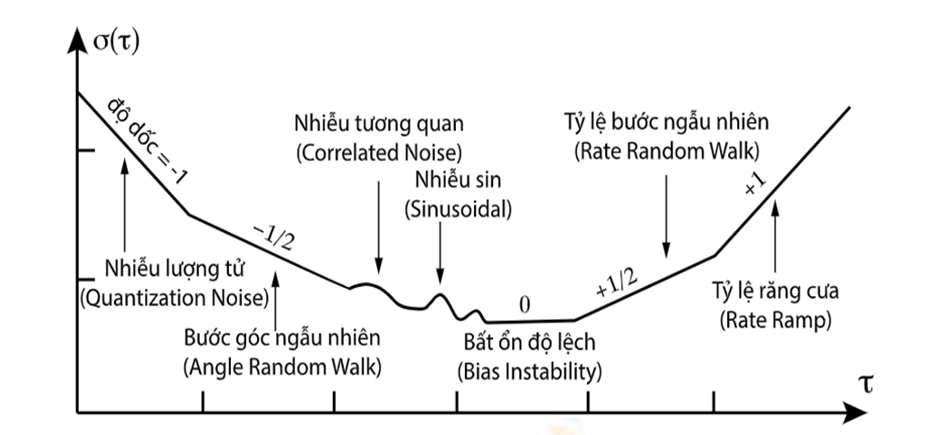
\includegraphics[width=\textwidth]{images/allan.png}
    \caption{Minh hoạ kết quả phân tích đường cong Allan}
    \label{allan}
\end{figure}

\textbf{Phân tích sai số ngẫu nhiên.} Tác giả sử dụng phương sai Allan 
để phân tích các thành phần nhiễu trong dữ liệu cảm biến \cite{allan}. 
Đây là phương pháp phân tích miền thời gian phổ biến nhằm đánh giá độ 
ổn định tần số và định lượng các loại nhiễu khác nhau như nhiễu trắng, 
trôi ngẫu nhiên, và nhiễu lượng tử. Biểu đồ Allan log-log cho phép nhận 
diện các thành phần nhiễu thông qua độ dốc của từng đoạn đường cong.

Trong thử nghiệm, cảm biến được đặt cố định trong phòng ở điều kiện 
nhiệt độ ổn định, với tần số lấy mẫu 10 Hz, thu được tổng cộng 1.211.210 
mẫu. Kết quả biểu diễn trong Hình~\ref{allan_real} cho thấy nhiễu chiếm 
ưu thế là nhiễu lượng tử (quantization noise), đặc trưng bởi hệ số góc 
tương ứng trong đồ thị.



\begin{figure}[htbp]
    \centering
    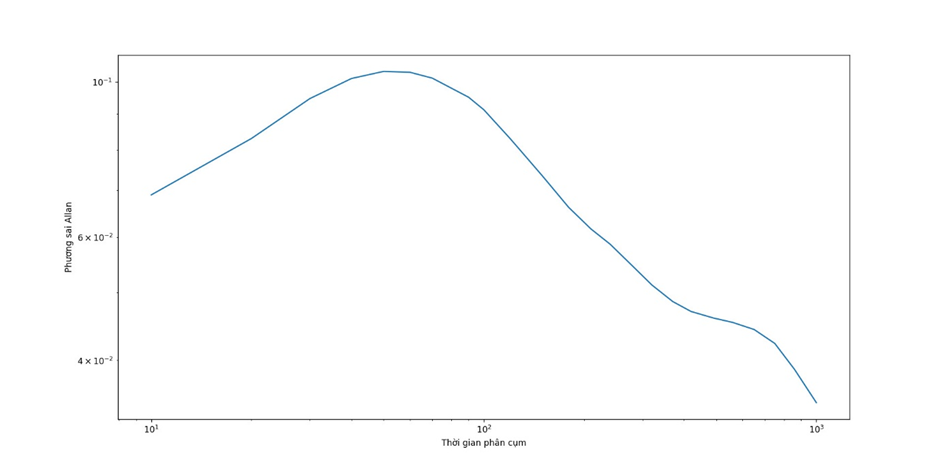
\includegraphics[width=\textwidth]{images/allan_real.png}
    \caption{Biểu đồ phương sai Allan của trục X}
    \label{allan_real}
\end{figure}

\textbf{Lọc nhiễu bằng bộ lọc Kalman.} Để xử lý nhiễu, đặc biệt là nhiễu 
lượng tử, tác giả sử dụng bộ lọc Kalman \cite{kalman}. Đây là một bộ lọc 
đệ quy có khả năng ước lượng trạng thái tối ưu của hệ thống từ các chuỗi 
đo lường bị nhiễu. Bộ lọc Kalman không chỉ phù hợp cho hệ thống tuyến 
tính mà còn có thể áp dụng cho hệ thống phi tuyến thông qua tuyến tính 
hoá cục bộ.

Trong hệ thống đề xuất, tín hiệu sau khi được cảm biến thu nhận sẽ 
được lọc trực tiếp tại vi điều khiển trước khi truyền đến ứng dụng 
để hiển thị và lưu trữ. Kết quả sau lọc được minh hoạ trong 
Hình~\ref{kalman}, cho thấy sự cải thiện đáng kể về độ mượt và ổn 
định của tín hiệu.


\begin{figure}[htbp]
    \centering
    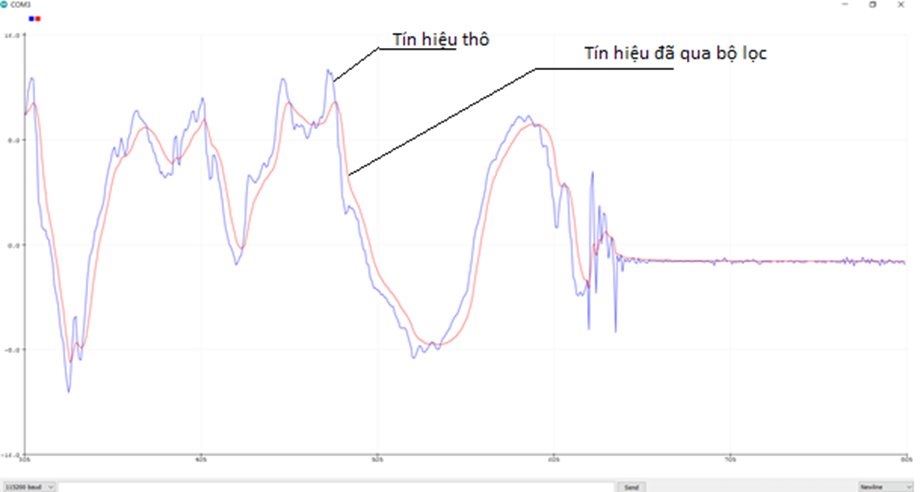
\includegraphics[width=\textwidth]{images/kalman.png}
    \caption{Kết quả bộ lọc Kalman cho dữ liệu trục X của cảm biến gia tốc}
    \label{kalman}
\end{figure}





\subsection{Xây dựng phần mềm ứng dụng}

Phần mềm ứng dụng được xây dựng với mục tiêu hỗ trợ người dùng trong việc 
kết nối với thiết bị phần cứng và trực quan hoá dữ liệu cảm biến. 
Ứng dụng đảm nhiệm vai trò là cầu nối giữa người dùng và hệ thống nhúng, 
đồng thời cung cấp các chức năng tương tác, cấu hình và theo dõi dữ liệu 
theo thời gian thực.

Các công nghệ và thành phần sử dụng được tóm tắt như sau:

\begin{flushleft}
\textbf{01)} Ngôn ngữ lập trình: \texttt{Dart} \\
\textbf{02)} Framework: \texttt{Flutter} \\
\textbf{03)} Nền tảng triển khai: \texttt{Android} \\
\textbf{04)} Giao tiếp phần cứng: Bluetooth Low Energy (BLE) \\
\textbf{05)} Chức năng chính: kết nối thiết bị, nhận dữ liệu, hiển thị, lưu trữ và cá nhân hóa trải nghiệm người dùng
\end{flushleft}

\begin{figure}[htbp]
    \centering
    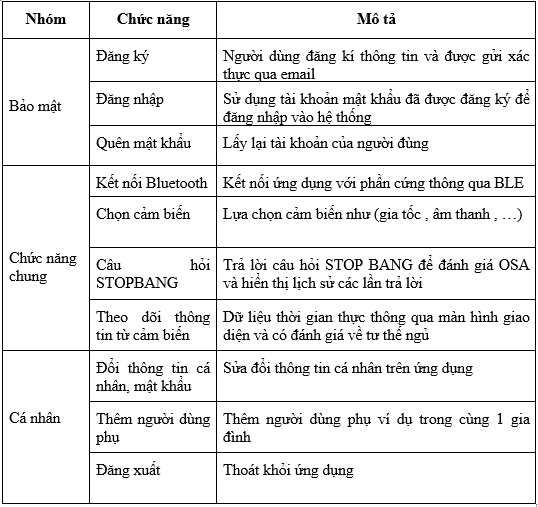
\includegraphics[width=\textwidth]{images/app_flow.png}
    \caption{Các nhóm chức năng chính của ứng dụng}
    \label{app_flow}
\end{figure}

Ứng dụng được thiết kế xoay quanh ba nhóm chức năng chính như minh họa 
trong Hình~\ref{app_flow}:

\begin{flushleft}
\textbf{01)} Nhóm bảo mật: đăng nhập, xác thực và khôi phục tài khoản. \\
\textbf{02)} Nhóm chức năng chung: kết nối với thiết bị phần cứng, thu thập và hiển thị dữ liệu cảm biến. \\
\textbf{03)} Nhóm cá nhân hoá: theo dõi chỉ số sức khỏe, khai báo STOP-BANG, lưu hồ sơ người dùng.
\end{flushleft}

\subsubsection*{Kiến trúc phần mềm}
Ứng dụng sử dụng mô hình \textbf{BLoC (Business Logic Component)} để tách biệt giao diện 
người dùng và logic xử lý. BLoC hoạt động dựa trên nguyên tắc nhận sự 
kiện đầu vào và trả về trạng thái phù hợp, giúp quản lý luồng dữ liệu 
hiệu quả. Cấu trúc tổng thể của kiến trúc BLoC gồm ba lớp chính được mô 
tả trong Hình~\ref{flutter}.

\begin{figure}[htbp]
    \centering
    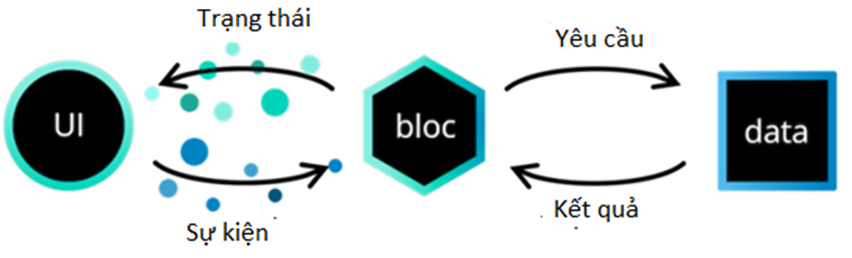
\includegraphics[width=0.8\textwidth]{images/flutter.png}
    \caption{Cấu trúc kiến trúc BLoC trong ứng dụng Flutter}
    \label{flutter}
\end{figure}


\begin{lstlisting}[float,language=dart,caption=Tập lệnh để tìm kiểm dịch vụ cảm biến ,label=flutterBle,captionpos=b]
StreamBuilder<List<BluetoothService>>(
      stream: device.services,
      initialData: [],
      builder: (c, snapshot) {
        if (snapshot.data!.length > 0) {
          isService = true;
        }
        BluetoothService serviceAcclerometer;
        if (snapshot.data == null || snapshot.data!.length == 0) {
          return Text("Please contact customer Service");
        }
        for (int i = 0; i < snapshot.data!.length; i++) {
          if (snapshot.data![i].uuid.toString() ==
              Constants.ACCLEROMETER_SERVICE) {
            accelerometerService = snapshot.data![i];
           }
        }
        if (accelerometerService == null) {
          return Text("Please contact customer Service");
        }
        for (int i = 0;
            i < accelerometerService!.characteristics.length;
            i++) {
          print(accelerometerService!.characteristics[i].uuid);
          if (accelerometerService!.characteristics[i].uuid
                  .toString() ==
              Constants.ACCLEROMETER_CHARACTION) {
            accelerometerCharactis =
                accelerometerService!.characteristics[i];
          }
        }
}));

\end{lstlisting}

\begin{lstlisting}[float,language=C,caption="Cấu trúc dữ liệu của phần nội dung đẩy lên máy chủ",label=format_ble,captionpos=b]
{
    "value": "0.88%0.66%0.99@2022-01-01/0.88%0.66%0.99@2022-01-01/0.88%0.66%0.99@2022-01-01",
    "customer": "62a5f5672ad9c724ef117d76"
}

\end{lstlisting}


Sau khi kết nối BLE được thiết lập thành công, ứng dụng truy xuất đối tượng đặc 
tính cảm biến (characteristic instance) và liên tục gửi yêu cầu đọc (\texttt{read}) 
đến vi điều khiển. Thiết bị phản hồi bằng cách trả về dữ liệu cảm biến 
dưới dạng mảng \texttt{UInt8}. Các giá trị này được ứng dụng giải mã, 
chuyển đổi sang dạng số thực tương ứng với gia tốc trên ba trục (X, Y, Z), 
và gắn nhãn thời gian thực.

Quá trình xử lý này được thực hiện trong một vòng 
lặp có kiểm soát độ trễ ngắn nhằm đảm bảo khả năng cập nhật liên tục 
nhưng vẫn tối ưu hiệu suất hệ thống.

Mã~\ref{flutterBle} minh hoạ toàn bộ quy trình xử lý: 
từ kết nối BLE, truy xuất đặc tính gia tốc, đọc giá trị nhị phân 
thô từ thiết bị, đến việc chuẩn hoá và gửi dữ liệu lên backend. 
Trong đoạn mã này, dữ liệu dạng \texttt{Uint8List} nhận từ cảm biến được tách và chuyển đổi 
thành ba thành phần tương ứng với ba trục gia tốc. Dữ liệu sau khi được xử lý sẽ được 
đóng gói theo định dạng \texttt{JSON} và gửi đến máy chủ thông qua phương thức 
POST, sử dụng thư viện \texttt{http} trong Flutter.

Định dạng dữ liệu BLE được chuẩn hoá như trong Mã~\ref{format_ble}, 
với trường \texttt{"value"} là chuỗi liên tục các 
giá trị cảm biến (phân tách bằng ký tự đặc biệt) và trường 
\texttt{"customer"} để định danh người dùng.

Việc tối ưu hóa cả quá trình đọc BLE và đẩy dữ liệu HTTP theo lô 
như vậy giúp giảm độ trễ, tránh tình trạng nghẽn băng thông, đồng thời 
vẫn đảm bảo độ chính xác và toàn vẹn của dữ liệu cảm biến.


Ngoài các chức năng thu thập và truyền dữ liệu cảm biến, ứng dụng còn tích hợp 
các công cụ hỗ trợ đánh giá y học lâm sàng ban đầu nhằm phục vụ cho việc sàng 
lọc và phân loại nguy cơ mắc hội chứng ngưng thở khi ngủ (OSA). Trong đó, 
ba thành phần quan trọng được triển khai bao gồm:

\noindent\textbf{01)} Bộ câu hỏi \textbf{STOP-BANG}: Đây là một bảng sàng lọc lâm sàng được sử dụng phổ biến trong y học giấc ngủ để đánh giá nguy cơ mắc OSA. Dữ liệu từ bảng này được lưu trữ cùng với dữ liệu cảm biến và đóng vai trò như đầu vào bổ sung cho các mô hình học máy dự đoán chỉ số AHI (Apnea–Hypopnea Index).

\vspace{0.5em}
\noindent\textbf{02)} Thang điểm \textbf{Epworth Sleepiness Scale (ESS)}: Tác giả triển khai thêm bảng câu hỏi ESS nhằm đánh giá mức độ buồn ngủ ban ngày của người dùng. Thang điểm này giúp phát hiện tình trạng buồn ngủ quá mức và có thể hỗ trợ phân tầng nguy cơ trong mô hình phân loại rối loạn giấc ngủ.

\vspace{0.5em}
\noindent\textbf{03)} Đánh giá \textbf{BMI (Body Mass Index)}: BMI được tự động tính toán dựa trên chiều cao và cân nặng người dùng nhập vào. Chỉ số này đóng vai trò là một trong các yếu tố nguy cơ chính trong chẩn đoán OSA, đặc biệt khi kết hợp cùng STOP-BANG.


Ngoài ra, nhằm cải thiện trải nghiệm người dùng và hỗ trợ trả lời câu hỏi liên quan 
đến giấc ngủ, tác giả 
phát triển thêm tính năng \textbf{chatbot y học giấc ngủ} dựa trên kỹ thuật 
\textbf{Retrieval-Augmented Generation (RAG)}. Chatbot này được xây dựng từ cơ 
sở dữ liệu gồm hơn 2000 câu hỏi và 
câu trả lời chuyên sâu liên quan đến giấc ngủ được biên tập bởi GS.TS Dương Quý Sỹ, 
bao gồm cả tài liệu lâm sàng, nghiên cứu khoa học và các hướng dẫn thực hành. 
Người dùng có thể đặt câu hỏi tự nhiên như “Tôi có nên lo nếu ngủ ngáy liên tục?” 
hoặc “STOP-BANG > 5 có ý nghĩa gì?”, và chatbot sẽ phản hồi dựa trên kiến 
thức được truy xuất từ tài liệu nền và được tổng hợp lại bằng mô hình ngôn ngữ.

Hệ thống RAG kết hợp khả năng truy vấn ngữ nghĩa từ tập văn bản lớn 
(document retrieval) và khả năng sinh văn bản linh hoạt từ mô hình ngôn ngữ lớn 
(LLM), từ đó cung cấp các câu trả lời chính xác, có căn cứ và dễ hiểu cho 
người dùng không chuyên.

\textbf{Tính năng quản lý người dùng} cũng được mở rộng. Người dùng có thể 
tạo tài khoản một lần và sử dụng lại trong các lần đăng nhập sau. Cơ chế này 
giúp rút ngắn thao tác, đồng thời vẫn đảm bảo tính bảo mật và khả năng khôi 
phục dữ liệu khi quên tài khoản hoặc mật khẩu. Dữ liệu người dùng 
(câu hỏi, chỉ số BMI, lịch sử cảm biến) được liên kết thống nhất qua một 
ID định danh duy nhất, hỗ trợ tốt cho việc phân tích, theo dõi tiến triển 
và huấn luyện mô hình học máy cá nhân hoá trong tương lai.



\subsection{Thiết kế và xây dựng hệ thống lưu trữ}
\begin{figure}[htbp]
    \centering
    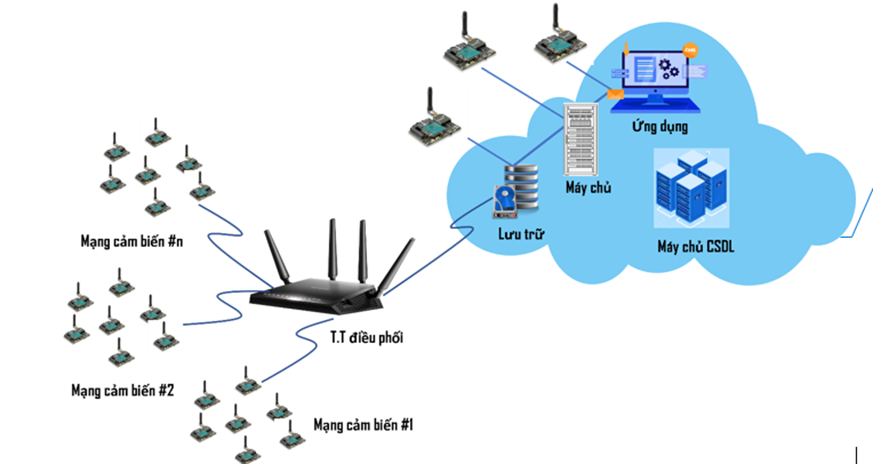
\includegraphics[width=0.8\textwidth]{images/cloud.png}
    \caption{Mô hình tích hợp giữa mạng cảm biến và cấu trúc dữ liệu đám mây}
    \label{cloud}
\end{figure}

Trong hệ thống đề xuất, dữ liệu cảm biến đóng vai trò trung tâm trong việc 
huấn luyện và triển khai các mô hình trí tuệ nhân tạo (AI). Tuy nhiên, bộ nhớ 
của vi điều khiển và thiết bị đầu cuối thường bị giới hạn, do đó giải pháp lưu 
trữ dữ liệu trên nền tảng đám mây là lựa chọn phù hợp và linh hoạt. Việc triển 
khai dữ liệu lên cloud không chỉ giúp loại bỏ rào cản về địa lý, mà còn hỗ 
trợ truy cập, phân tích và chia sẻ dữ liệu từ bất kỳ đâu miễn có kết nối 
Internet. Đồng thời, hệ thống hỗ trợ xuất dữ liệu dưới dạng văn bản (text), 
CSV hoặc JSON, phục vụ nhu cầu chia sẻ giữa các nhóm nghiên cứu.

Về dài hạn, mục tiêu của hệ thống là tích luỹ một tập dữ liệu lớn và đa dạng 
nhằm huấn luyện các mô hình học máy hỗ trợ chẩn đoán và ra quyết định trong 
sàng lọc hội chứng ngưng thở khi ngủ (\gls{OSA}).



\textbf{Cơ sở dữ liệu sử dụng là MongoDB Atlas} với các đặc điểm kỹ thuật nổi bật như sau:
01) Hỗ trợ lưu trữ hiệu quả dữ liệu lớn, phân tán trên nhiều cụm máy chủ, 
cho phép mở rộng theo chiều ngang.
02) Tối ưu hoá truy vấn theo thời gian thực với dữ liệu dạng \texttt{timestamp}.
03) Cơ chế đánh chỉ mục linh hoạt giúp tăng tốc độ truy vấn và giảm dung lượng lưu trữ.
04) Hỗ trợ tự động xoá dữ liệu cũ dựa trên TTL (Time To Live index), 
đồng thời tích hợp trực tiếp với nền tảng MongoDB Atlas.

\begin{figure}[htbp]
\centering
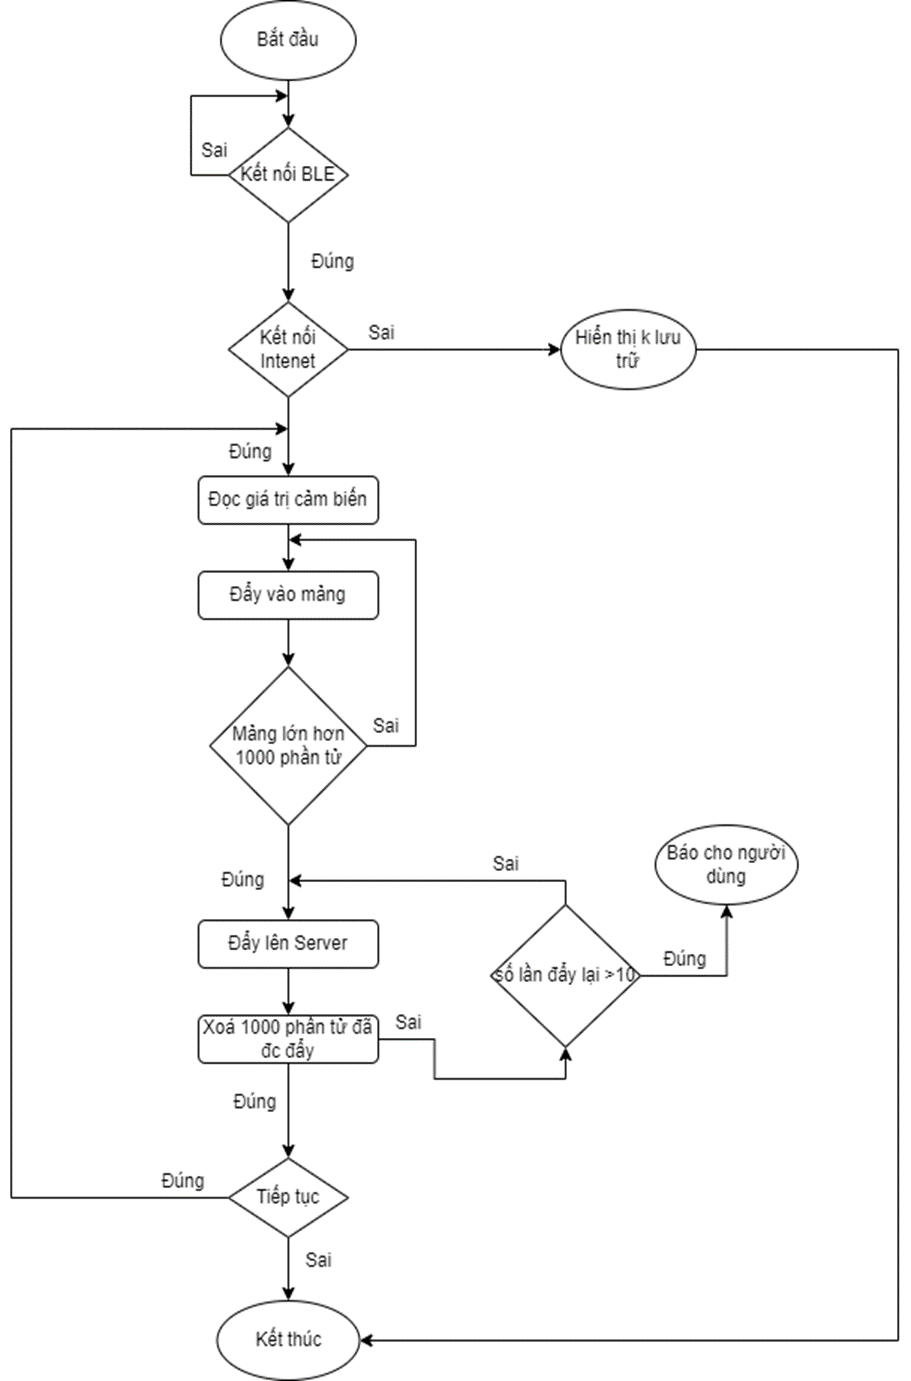
\includegraphics[width=0.9\textwidth]{images/flow_http.png}
\caption{Lưu đồ thuật toán lưu trữ dữ liệu cảm biến}
\label{flow_http}
\end{figure}
Phía máy chủ của hệ thống được xây dựng bằng nền tảng Node.js và triển khai 
trên Amazon Web Services (AWS), cho phép triển khai nhanh, dễ mở rộng và tối 
ưu chi phí trong giai đoạn thử nghiệm. MongoDB Atlas được lựa chọn là hệ quản 
trị cơ sở dữ liệu chính, hỗ trợ gói miễn phí dung lượng 500MB – phù hợp cho 
việc thu thập và đánh giá dữ liệu ở quy mô ban đầu.

Để tránh tình trạng quá tải server khi có nhiều yêu cầu truy cập đồng thời, 
ứng dụng không thực hiện gửi từng mẫu riêng lẻ. Thay vào đó, dữ liệu cảm biến 
sẽ được tích luỹ theo từng lô gồm 1000 mẫu, sau đó mới được gửi lên backend. 
Mỗi mẫu bao gồm ba thành phần gia tốc (\texttt{x, y, z}) và thời gian ghi 
nhận tương ứng, bảo đảm tính toàn vẹn và khả năng truy xuất ngược theo dòng 
thời gian.

Lưu đồ thuật toán lưu trữ dữ liệu được thể hiện trong Hình~\ref{flow_http}, 
gồm hai trường hợp chính:

\vspace{0.5em}
\noindent\textbf{1)} Khi người dùng không có kết nối mạng, hệ thống vẫn cho phép kết nối BLE và hiển thị dữ liệu cảm biến theo thời gian thực, tuy nhiên sẽ không tiến hành lưu trữ lên cloud.

\vspace{0.5em}
\noindent\textbf{2)} Khi người dùng đã đăng nhập và có kết nối Internet, ứng dụng sẽ tự động lưu trữ dữ liệu sau mỗi 1000 mẫu thu thập. Trong trường hợp thao tác gửi dữ liệu thất bại liên tục quá 10 lần, hệ thống sẽ thông báo lỗi và ngừng tiến trình lưu trữ để đảm bảo độ tin cậy.


Ngoài dữ liệu cảm biến thời gian thực được lưu trữ trên MongoDB Atlas, 
hệ thống còn sử dụng cơ sở dữ liệu quan hệ MySQL để quản lý các dữ liệu định 
danh và nghiệp vụ quan trọng khác. Cụ thể:

\vspace{0.5em}
\noindent\textbf{1)} Thông tin người dùng như tài khoản đăng nhập, mật khẩu mã hoá (hash), email, số điện thoại, lịch sử đăng nhập và phân quyền được lưu trữ trong hệ quản trị cơ sở dữ liệu MySQL. Cấu trúc dữ liệu dạng bảng (table) của MySQL giúp đảm bảo tính toàn vẹn quan hệ và dễ dàng thực hiện các truy vấn xác thực người dùng nhanh chóng, an toàn.

\vspace{0.5em}
\noindent\textbf{2)} Các dữ liệu khảo sát lâm sàng như bảng điểm STOP-BANG, thang điểm Epworth, chỉ số BMI, tiền sử bệnh nền và lịch sử đánh giá lặp lại theo từng thời điểm cũng được lưu trong MySQL nhằm đảm bảo tính liên kết logic giữa các thực thể (người dùng – biểu mẫu – kết quả – thời gian).

\vspace{0.5em}
\noindent\textbf{3)} Việc phân chia lưu trữ theo đặc thù dữ liệu (NoSQL cho dữ liệu cảm biến lớn và động, SQL cho dữ liệu người dùng có cấu trúc ổn định) giúp tối ưu hoá hiệu suất truy xuất, tính mở rộng và khả năng bảo trì hệ thống trong dài hạn.

Sự kết hợp giữa MongoDB (dành cho dữ liệu cảm biến, thời gian thực) 
và MySQL (dành cho thông tin người dùng và nghiệp vụ) tạo thành một kiến trúc 
lưu trữ lai (hybrid storage architecture) đáp ứng linh hoạt cả hai loại dữ 
liệu – phi cấu trúc và có cấu trúc – vốn là đặc trưng phổ biến trong các 
hệ thống y tế ứng dụng trí tuệ nhân tạo hiện đại.

\subsection{Tìm hiểu, ứng dụng phân loại tư thế ngủ bằng học máy  }

Tác giả cũng đã tìm hiểu nhiều mô hình, phương pháp để phân loại các tư thế ngủ, tư thế cơ bản của con người và đánh giá chỉ số AHI dự trên các tín hiệu cảm biến thu được. Các bước cơ bản để tiến hành dự án học máy liên quan đến các tín hiệu cảm biến:


\begin{figure}[b!]
		\centering
 		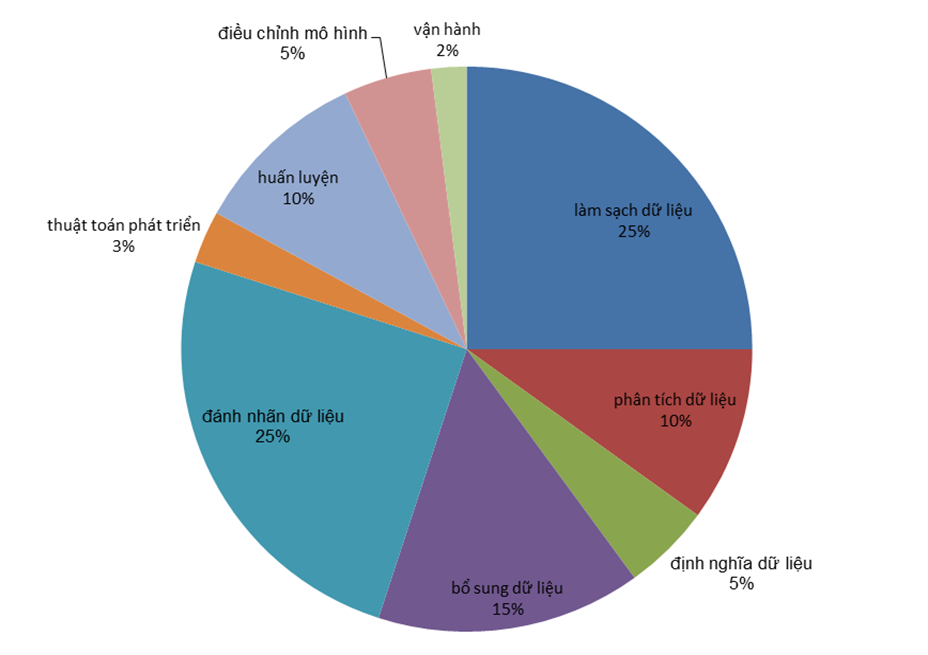
\includegraphics[width=1\textwidth]{images/hocmay_time.png}
		\caption{Phân bố thời gian sử dụng đối với dự án học máy}
		\label{hocmay_time}
\end{figure}

\begin{itemize}
    \item Thu thập dự liệu (bao gồm thu thập và gắn nhãn cho dữ liệu)
    
    \item Khám phá dữ liệu (đánh giá cân bằng dữ liệu, tỉ lệ dữ liệu có ý nghĩa)
    
    \item Chuẩn bị dữ liệu (làm sạch dữ liệu, tạo ra các đặc tính trên miền thời gian và miền tần số)
    
    \item Mô hình hoá dữ liệu (lựa chọn ra các mô hình phù hợp)
    
    \item Lựa chọn tính năng (lựa chọn ra các tính năng có ý nghĩa cao đối với mô hình)

    \item Tinh chỉnh mô hình
\end{itemize}

Jeng PY và cộng sự đã đề xuất chế tạo 2 thiết bị đeo ở cổ và ở cổ tay để đánh giá tư thế ngủ ở người \cite{Jeng}. Trong dự án này, tín hiệu thu được ở thiết bị đeo ở tay được chia thành những cửa sổ 1 giây rồi trích xuất các tính năng trên cửa sổ đó. Cảm biến đeo ở cổ sẽ được sử dụng để lấy nhãn tín hiệu theo phương pháp lấy đa số của tín hiệu trong cửa sổ. Nhóm tác giả đã sử dụng mô hình SVM và RF để đánh giá và đạt được kết quả có độ chính xác lần lượt là 82\% và 72\%. Nhóm của Saha S., Kabir M và cộng sự đã tiến hành nghiên cứu 1 thiết bị đeo được sử dụng bao gồm cảm biến gia tốc, cảm biến âm trên 31 đối tượng thử nghiệm. Sau đó họ tiến hành loại bỏ các bộ dữ liệu có độ dài dưới 2 giờ và cuối cùng sử dụng so sánh ngưỡng để xác định chứng OSA bằng việc phân chia các cửa sổ 10s với độ lặp 80\% \cite{Saha}. Trong khi đó, nhóm của Syeda Zuriat-e-Zehra Ali và cộng sử đã nghiên cứu và thử nghiệm thiết bị gối ngủ để tự điều chỉnh hoặc báo hiệu khi có chứng ngưng thở khi ngủ dựa trên các tín hiệu thô như nồng độ Oxi trong máu, nhịp tim [27]. Jarvis L, Moninger S và cộng sử đã trình bày hệ thống phát hiện đánh giá 5 tư thế gồm nằm, nằm tựa, ngồi thẳng, đứng, đi bộ với tập dữ liệu đươc lấy từ 2 cảm biến gắn ở cổ và đùi \cite{Syeda}. Dữ liệu được lấy mẫu với tần số 25 Hz sau đó được lưu vào bộ nhớ cục bộ trên điện thoại rồi gửi bản csv qua mail. Mô hình học máy gồm hồi quy logistic, SVM, DT với độ chính xác cao > 96\% đã được sử dụng đánh giá tập dữ liệu gồm 6 hành động thường ngày của con người như đứng, ngồi, đi bộ, lên cầu thang, xuống cầu thang và nằm \cite{Uday}. Nhóm nghiên cứu của Gomes E, Bertini L và cộng sự đã nghiên cứu, xây dựng, đánh giá giữa 3 mô hình: K-Nearest-Neighbor (KNN), cây quyết định (Decision tree) và SVM. Trong các bước tiền xử lý các tác giả đã phân đoạn dữ liệu theo cửa sổ 2.5s không che phủ sau đó phân tích, chuẩn hoá dữ liệu và đã có độ chính xác > 97\% đối với việc phát hiện tư thế. Ở Việt Nam, nhóm tác gủa Vũ Ngọc Thanh Sang và Nguyễn Đức Thắng đã phát triển thiết bị thu thâp dữ liệu từ điện thoại sau đó qua các bước xử lý dữ liệu, trích xuất tính năng và phân loại bằng các mô hình K-hàng xóm gần nhất (KNN) với độ chính xác là 100\% với toàn bộ tư thế ngoại trừ lái xe là 80\% \cite{Sang}. Qua tổng quan tài liệu tác giả nhận thấy các phương pháp học máy cổ điển đang chiến ưu thế hơn so với các phương pháp học sâu vì phát triển nhanh và dễ dàng và phù hợp với tính chất của bài toán đánh giá các tư thế của con người sử dụng cảm biến gia tốc. Trong đó, nổi bật lên là mô hình SVM, hồi quy Logistic và Random Forest. Từ đó, tác giả sẽ tập trung tìm hiểu và hướng tới áp dụng cho tập dữ liệu của tác giả.


\textbf{Hồi quy logistic - LR}: Đây là phương thức tốt nhất cho các vấn đề phân loại nhị phân (vấn đề với hai lớp giá trị). Hồi quy logistic giống như hồi quy tuyến tính với mục đích là để tìm ra các giá trị cho các hệ số mà trọng lượng mỗi biến đầu vào. Không giống như hồi quy tuyến tính, dự đoán đầu ra được chuyển đổi bằng cách sử dụng một hàm không tuyến tính được gọi là hàm logistic. Hàm logistic trông giống như một chữ S lớn và sẽ biến đổi bất kỳ giá trị nào thành 0-1. Tuy nhiên, nhược điểm của nó là chỉ giải quyết được bài toán phân loại 2 lớp. Để giải quyết được những bài toán đa lớp chúng ta có thể sử dụng mô hình Softmax Logistic là dạng tổng quát của hồi quy Logistic.

\textbf{Máy vec tơ hỗ trợ (Support vector machines - SVM)}: xây dựng một mặt siêu phẳng được sử dụng để phân chia không gian biến đầu vào. Trong SVM, một mặt siêu phẳng được chọn để phân tách tốt nhất các điểm trong không gian các biến đầu vào theo lớp của chúng, hoặc là lớp 0 hoặc lớp 1. Trong không gian hai chiều, có thể hình dung nó như một đường thẳng và giả sử rằng tất cả các biến đầu vào có thể được tách hoàn toàn bằng đường thẳng này. Thuật toán SVM tìm ra các hệ số dẫn đến sự phân tách tốt nhất của các lớp theo mặt siêu phẳng Hình ~\ref{svm}.


\begin{figure}
    \centering
    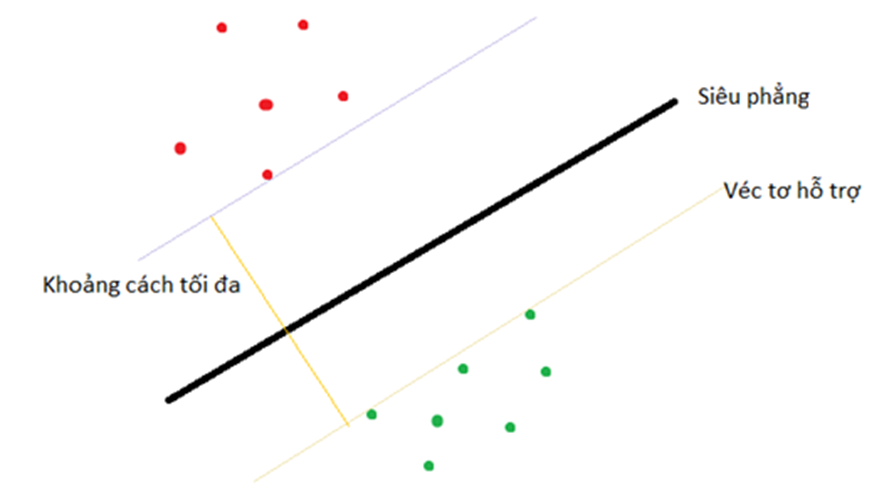
\includegraphics[width=1\linewidth]{images/svm.png}
    \caption{Tối ưu siêu phẳng sử dụng thuật toán SVM}
    \label{svm}
\end{figure}
Khoảng cách giữa mặt siêu phẳng và điểm dữ liệu gần nhất được gọi là biên. Mặt siêu phẳng tốt nhất hoặc tối ưu có thể tách riêng hai lớp là dòng có biên lớn nhất. Chỉ những điểm này có liên quan đến việc xác định hyperplane và trong việc xây dựng các điểm phân loại. Những điểm này được gọi là các vector hỗ trợ. Chúng hỗ trợ hoặc xác định hyperplane. Trong thực tế, một thuật toán tối ưu được sử dụng để tìm các giá trị cho các hệ số tối đa hóa biên. SVM có thể là một trong những phương pháp phân loại hàng đầu mạnh mẽ nhất và đáng thử trên tập dữ liệu. Cũng như hồi quy Logistic thì SVM cũng chỉ sử dụng để phân loại nhị phân. Để giải quyết vấn đề này thì có 2 phương pháp:

\begin{figure}
    \centering
    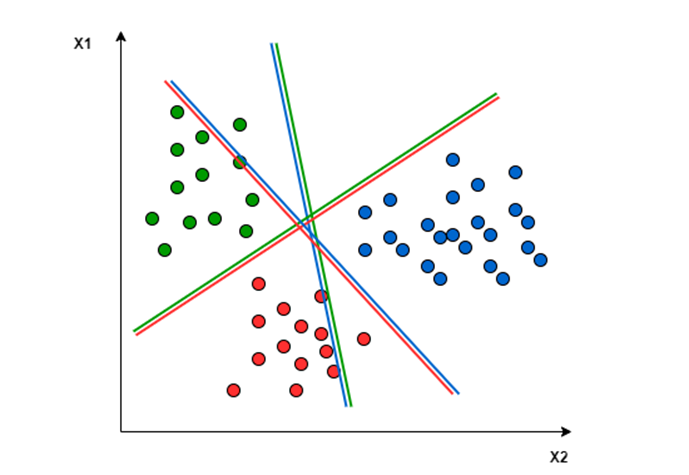
\includegraphics[width=0.6\linewidth]{images/svm_ovso.png}
    \caption{Thuật toán một với một}
    \label{svm_ovso}
\end{figure}



\begin{figure}
    \centering
    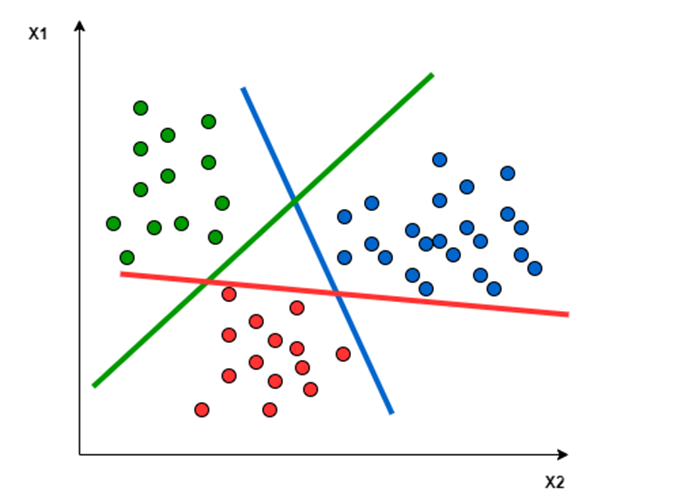
\includegraphics[width=0.6\linewidth]{images/ovsr.png}
    \caption{Thuật toán một với nhiều}
    \label{ovsr}
\end{figure}

\begin{itemize}
    \item Một với một (one vs one): Một mặt siêu phẳng được thiết lập để phân tách giữa hai lớp, bỏ qua các điểm của lớp thứ ba. Điều này có nghĩa là sự phân tách chỉ tính đến điểm của hai lớp trong sự phân tách hiện tại. Ví dụ: đường màu đỏ-xanh dương sẽ tách tối đa khoảng cách chỉ giữa các điểm màu xanh lam và màu đỏ Hình ~\ref{svm_ovso}.
    
    \item Một với nhiều (one vs rest): Cần một mặt siêu phẳng để tách biệt giữa một lớp và tất cả các lớp khác cùng một lúc. Điều này có nghĩa là sự tách biệt có tính đến tất cả các điểm, chia chúng thành hai nhóm; một nhóm cho các điểm của lớp và một nhóm cho tất cả các điểm khác. Ví dụ: đường màu sẽ tách tối đa hóa khoảng cách giữa các điểm màu lục và tất cả các điểm khác cùng một lúc Hình ~\ref{ovsr}.
\end{itemize}






\textbf{Rừng ngẫu nhiên (Random Forest - RF)}: được xây dựng trên cơ sở thuật toán Decision Tree (cây quyết định). Mỗi cây quyết định sẽ khác nhau (có yếu tố ngẫu nhiên khác nhau). Sau đó kết quả dự đoán được tổng hợp từ các cây quyết định. Trong thuật toán Decision Tree, khi xây dựng cây quyết định nếu để độ sâu tùy ý thì cây sẽ phân loại đúng hết các dữ liệu trong tập training dẫn đến mô hình có thể dự đoán tệ trên tập validation/test, khi đó mô hình bị quá khớp (overfitting).
Thuật toán Random Forest gồm nhiều cây quyết định, mỗi cây quyết định đều có những yếu tố ngẫu nhiên:
Lấy ngẫu nhiên dữ liệu để xây dựng cây quyết định.
Lấy ngẫu nhiên các thuộc tính để xây dựng cây quyết định.
Do mỗi cây quyết định trong thuật toán Random Forest không dùng tất cả dữ liệu training, cũng như không dùng tất cả các thuộc tính của dữ liệu để xây dựng cây nên mỗi cây có thể sẽ dự đoán không tốt, khi đó mỗi mô hình cây quyết định không bị overfitting mà có thế bị underfitting, hay nói cách khác là mô hình có high bias. Tuy nhiên, kết quả cuối cùng của thuật toán Random Forest lại tổng hợp từ nhiều cây quyết định, thế nên thông tin từ các cây sẽ bổ sung thông tin cho nhau, dẫn đến mô hình có low bias và low variance, hay mô hình có kết quả dự đoán tốt.
	Những kiến thức cơ bản về học máy sẽ được ứng dụng sâu trong những nghiên cứu tới đây của tác giả.



\chapter{KẾT QUẢ THỰC NGHIỆM VÀ ĐÁNH GIÁ}
Trong phần này, tác giả trình bày các kết quả đạt được từ hai giai đoạn chính: 
(i) thu thập và xử lý dữ liệu cảm biến từ các tư thế ngủ khác nhau; 
(ii) huấn luyện mô hình học máy và triển khai mô hình tối ưu lên vi điều khiển nhằm đánh giá tính khả thi của giải pháp trên thiết bị biên.

\section{Hệ thống thực nghiệm}

\begin{figure}[htbp]
    \centering
    \begin{subfigure}[b]{0.45\linewidth}
        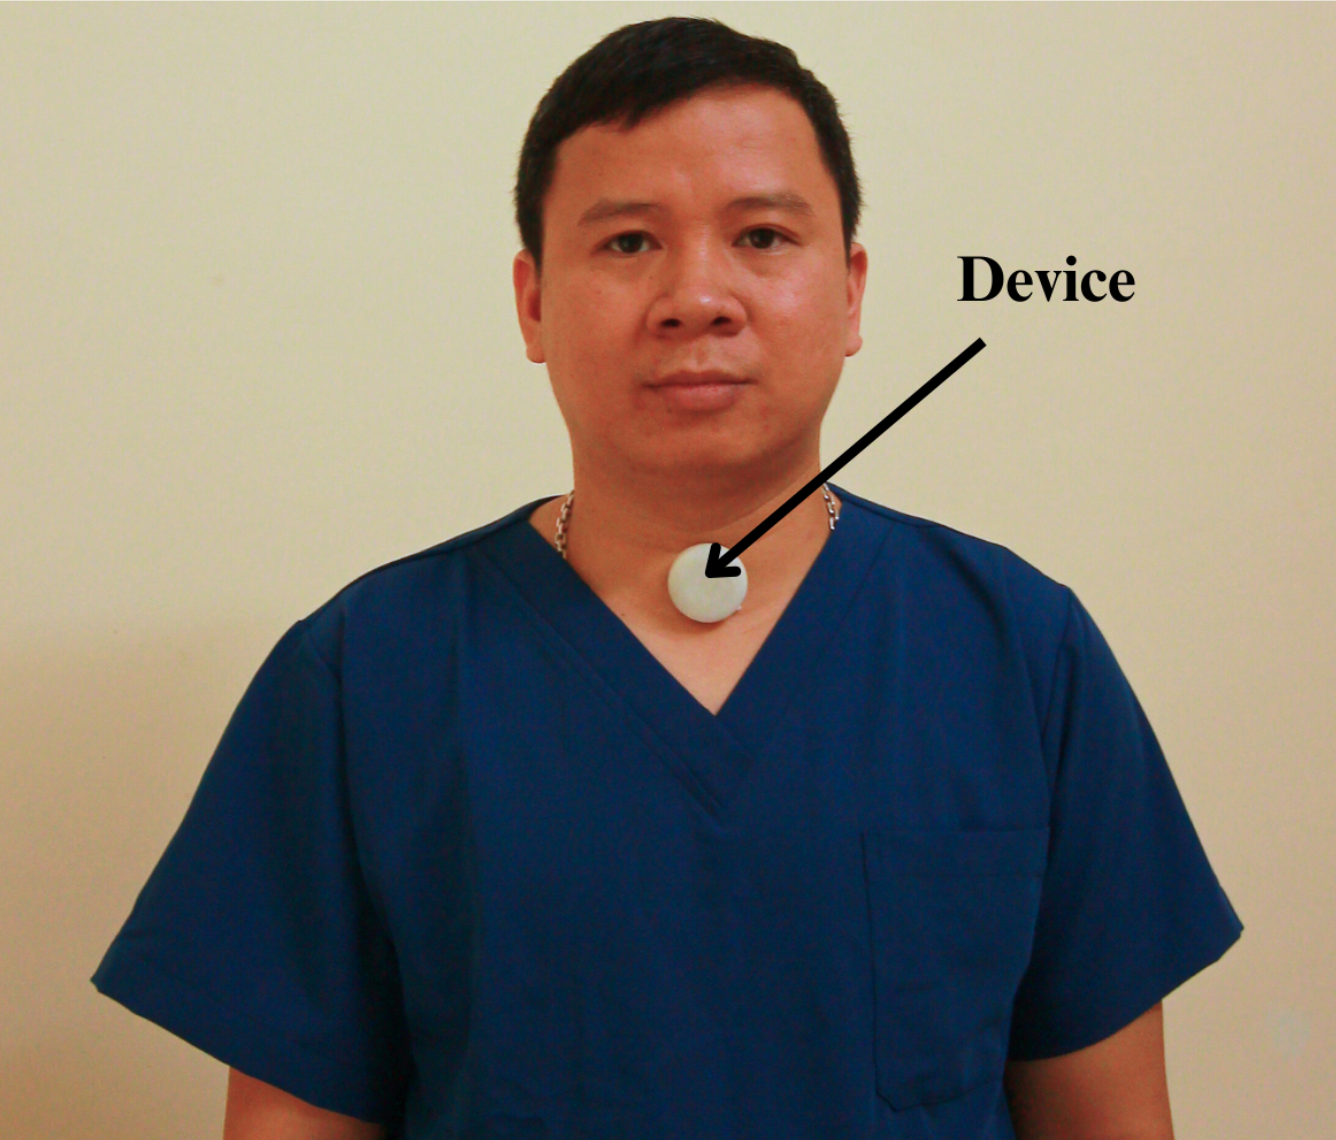
\includegraphics[width=\linewidth,height=6cm,keepaspectratio]{images/sleepdive2.png}
        \caption{}
        \label{fig:device_position}
    \end{subfigure}
    \hfill
    \begin{subfigure}[b]{0.45\linewidth}
        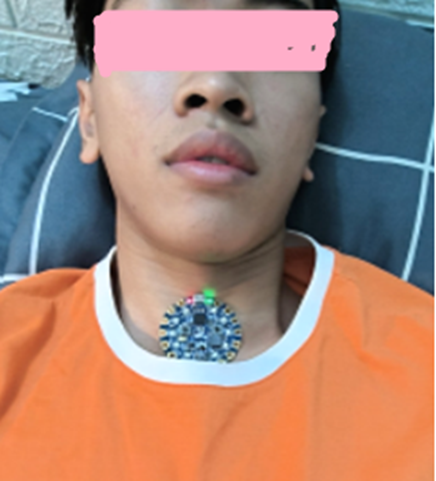
\includegraphics[width=\linewidth,height=6cm,keepaspectratio]{images/thucnghiem.png}
        \caption{}
        \label{fig:practical_test}
    \end{subfigure}
    \caption{Hệ thống thử nghiệm: (a) vị trí đặt thiết bị cảm biến; (b) minh hoạ thực nghiệm thực tế trong tư thế nằm.}
    \label{fig:experiment_system}
\end{figure}

Tác giả đã hoàn thiện việc lập trình firmware cho bộ vi mạch cảm biến 
tích hợp vi điều khiển NRF52840 và cảm biến gia tốc ba trục LIS3DH. 
Firmware được xây dựng sử dụng ngôn ngữ C/C++ trên nền tảng Arduino Core, 
tối ưu hóa để vận hành ổn định trong môi trường năng lượng thấp và 
hỗ trợ giao tiếp không dây chuẩn Bluetooth Low Energy (BLE).

Để đảm bảo khả năng hoạt động liên tục trong suốt một đêm ngủ 
(tối thiểu 8 giờ), hệ thống được thiết kế sử dụng pin cúc áo CR2032, 
với dòng tiêu thụ trung bình được đo đạt dưới 8 mA trong chế độ 
ghi nhận liên tục và truyền dữ liệu định kỳ.

Mã nguồn firmware bao gồm các khối chức năng chính: 
khởi tạo cảm biến, hiệu chỉnh dải đo và tần số lấy mẫu (10~Hz), 
lọc nhiễu đầu vào (bằng kỹ thuật trung bình trượt), 
đóng gói dữ liệu,
và truyền dữ liệu qua BLE đến ứng dụng Android. 
Ngoài ra, tác giả cũng tích hợp cơ chế báo hiệu bằng LED để xác nhận 
trạng thái hoạt động của thiết bị (kết nối, truyền dữ liệu, và lỗi).
Kết quả thử nghiệm thực tế cho thấy hệ thống hoạt động ổn định 
trong suốt thời gian ghi nhận dữ liệu qua đêm, không xảy ra hiện tượng 
rớt kết nối hay tràn bộ đệm dữ liệu. Toàn bộ dữ liệu thu được được đồng 
bộ theo thời gian thực tới ứng dụng di động, phục vụ cho các giai đoạn 
xử lý tín hiệu và huấn luyện mô hình học máy ở các chương sau.


Một trong các nhiệm vụ chính mà tác giả thực hiện là phát triển ứng dụng 
di động phục vụ cho quá trình thu thập, hiển thị và xử lý dữ liệu. 
Dựa trên phản hồi từ nhóm nghiên cứu, tư vấn khoa học của Thầy PGS.TS. Mai Anh Tuấn, tư vấn
y khoa của Thầy GS.TS. Dương Quý Sỹ,
ứng dụng được thiết kế với tiêu 
chí giao diện thân thiện, thao tác đơn giản và tính năng tập trung vào 
mục tiêu thử nghiệm.

Sau khi cài đặt, người dùng có thể đăng nhập hoặc đăng ký tài khoản 
thông qua giao diện như được thể hiện trong Hình~\ref{appAuth}. 
Với người dùng mới, quá trình đăng ký yêu cầu xác thực địa chỉ 
email nhằm đảm bảo bảo mật và hỗ trợ tính năng khôi phục tài khoản.
Hình ~\ref{app_cate} là giao diện khi người dùng đăng nhập thành công, 
bao gồm các tính năng: Kết nối BLE và đọc dữ liệu, chuyển người dùng, 
xem thông tin người dùng v.v.
Hình ~\ref{listble} thể hiện danh sách BLE có thể kết nối và 
dịch vụ kết nối với phần cứng đã được nhắc tới bên trên.


\begin{figure}[htbp]
    \centering
    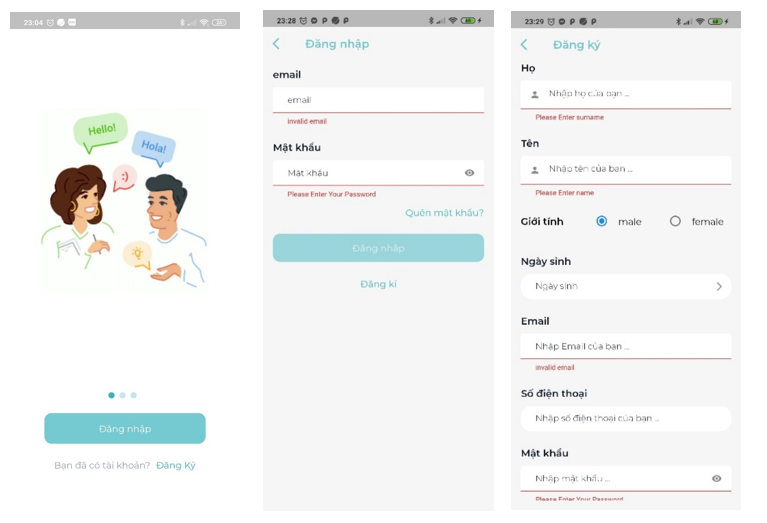
\includegraphics[width=0.8\linewidth]{images/appAuth.png}
    \caption{Giao diện chức năng đăng ký và đăng nhập}
    \label{appAuth}
\end{figure}

\begin{figure}[h!]
    \centering
    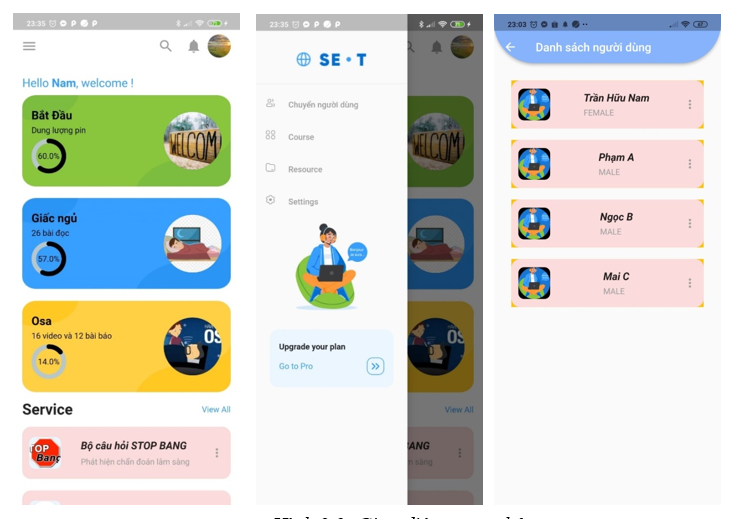
\includegraphics[width=0.8\linewidth]{images/app_cate.png}
    \caption{Giao diện trang chủ}
    \label{app_cate}
\end{figure}


\begin{figure}[htbp]
    \centering
    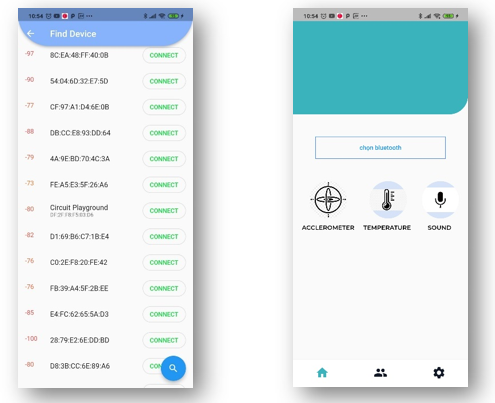
\includegraphics[width=0.5\linewidth]{images/app_ble.png}
    \caption{Giao diện màn hình danh sách BLE và chi tiết các dịch vụ kết nối với phần cứng}
    \label{listble}
\end{figure}

Hình~\ref{appsleep} minh họa giao diện của các chức năng hỗ trợ người 
dùng trong quá trình sàng lọc nguy cơ ngưng thở khi ngủ và cung cấp 
thông tin về chất lượng giấc ngủ. Giao diện đầu tiên (từ trái sang) 
hiển thị mục "Hỏi – Đáp về Giấc Ngủ", nơi người dùng có thể tra cứu 
các thông tin được tổng hợp từ chuyên gia trong lĩnh vực y học giấc ngủ. 
Giao diện thứ hai trình bày tập hợp các công cụ đo lường phổ biến như 
thang điểm Epworth, STOP-BANG, chỉ số khó có thể duy trì sự tỉnh táo 
(ESS), và các bộ câu hỏi dành riêng cho trẻ em hoặc đánh giá chất lượng 
giấc ngủ theo thang điểm Pittsburgh (PSQI).
Giao diện thứ ba mô tả chi tiết một bộ câu hỏi sàng lọc nguy cơ ngưng 
thở khi ngủ (tên mục: “Tầm soát ngày – Ngưng thở”) bao gồm các câu hỏi 
tổng quát và chuyên biệt nhằm đánh giá các yếu tố liên quan đến OSA 
(Obstructive Sleep Apnea), như tần suất ngáy, triệu chứng ngủ gật ban 
ngày, gián đoạn giấc ngủ, hoặc các đặc điểm nhân trắc học có liên quan.

Giao diện thứ tư là chức năng chatbot – nơi người dùng có thể trao 
đổi trực tiếp với hệ thống trí tuệ nhân tạo được lập trình sẵn để 
phản hồi các câu hỏi về OSA. Chatbot có khả năng nhận diện từ khóa 
và cung cấp phản hồi ngắn gọn dựa trên cơ sở dữ liệu đã huấn luyện. 
Trong ví dụ minh họa, chatbot phản hồi một truy vấn liên quan đến chỉ 
số BMI và nguy cơ mắc OSA, thể hiện vai trò hỗ trợ tư vấn bước đầu 
cho người dùng nghi ngờ có hội chứng ngưng thở khi ngủ.



\begin{figure}[htbp]
    \centering
    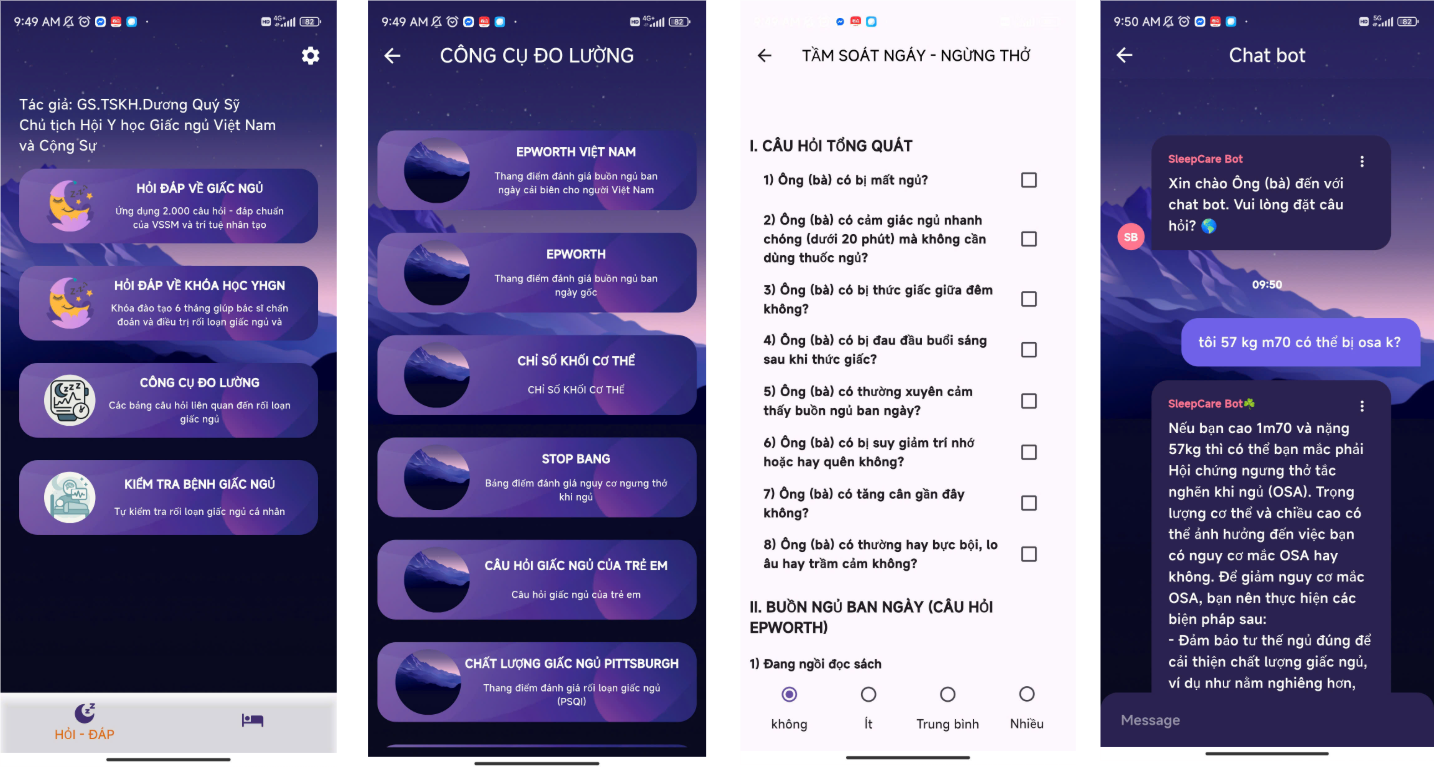
\includegraphics[width=0.8\linewidth]{images/appsleep.png}
    \caption{Giao diện chức năng chatbot và bộ câu hỏi tầm soát}
    \label{appsleep}
\end{figure}

\begin{lstlisting}[float,language=C,caption=Tập lệnh đánh giá tư thế ngủ bằng ngưỡng, label=nguong,captionpos=b]
static Function getPositionSleep = (double x, double y, double z) {
    if ((-6.5 < y && y < 6.5)) {
      if (-7.07 < x && x < 7.07) {
        if (z > 0) {
          return 1; // ngua
        }
        if (z < 0) {
          return 4; //sap
        }
      }
      if (x > 3) return 2; //trai
      if (x < -3) return 3; //phai
  }
    return 6; // khong phai nam
  };

\end{lstlisting}


Hình~\ref{appbieudo} minh họa giao diện hiển thị giá trị 
cảm biến theo thời gian thực. Phần đầu hiển thị biểu đồ ba trục 
x, y, z. Phần thứ hai là tổng thời gian theo từng tư thế ngủ 
được tính toán dựa trên tín hiệu nhận dạng. Phần cuối cùng cho biết 
tư thế hiện tại mà hệ thống đang xác định được. 
Tuy nhiên, phương pháp xác định tư thế dựa trên ngưỡng chưa có tính tổng quát cao. 
Do đó, trong các phần tiếp theo, các mô hình học máy sẽ 
được áp dụng để cải thiện độ chính xác và ổn định của hệ 
thống nhận diện tư thế. Việc cập nhật tư thế được thực hiện 
định kỳ mỗi 10 giây để tăng khả năng phản hồi theo thời gian thực.

\begin{figure}[htbp]
    \centering
    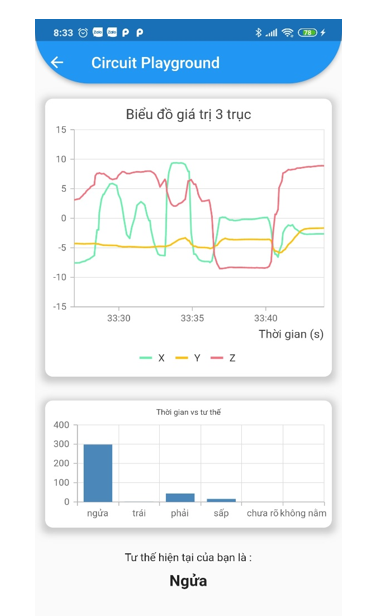
\includegraphics[width=0.3\linewidth]{images/appbieudo.png}
    \caption{Giao diện hiển thị dữ liệu gia tốc ba trục}
    \label{appbieudo}
\end{figure}

Về mặt kiến trúc lưu trữ dữ liệu, hệ thống được thiết kế phân tách 
giữa dữ liệu định tính và dữ liệu định lượng. Cụ thể, thông tin người 
dùng (tài khoản, cấu hình cá nhân), các bộ câu hỏi tầm soát 
(ví dụ: STOP-BANG, ESS), cùng với nội dung trả lời và phản hồi của 
chatbot được lưu trữ trong cơ sở dữ liệu quan hệ \textbf{PostgreSQL}. 
Cơ sở dữ liệu này hỗ trợ tính nhất quán cao và dễ dàng cho việc mở 
rộng truy vấn phức tạp trong các bài toán phân tích sau này.
Trong khi đó, dữ liệu cảm biến gia tốc được lưu trữ song song tại cơ 
sở dữ liệu phi quan hệ \textbf{MongoDB}, với định dạng BSON linh hoạt, 
phù hợp cho việc ghi nhận chuỗi thời gian lớn và truy xuất nhanh theo 
timestamp. Ngoài ra, hệ thống được mở rộng với các API cho phép trích 
xuất dữ liệu dưới dạng Excel, nhằm hỗ trợ phân tích và chia sẻ thông 
tin một cách linh hoạt.



\section{Thu thập và gắn nhãn dữ liệu}

\begin{figure}[htbp]
\centerline{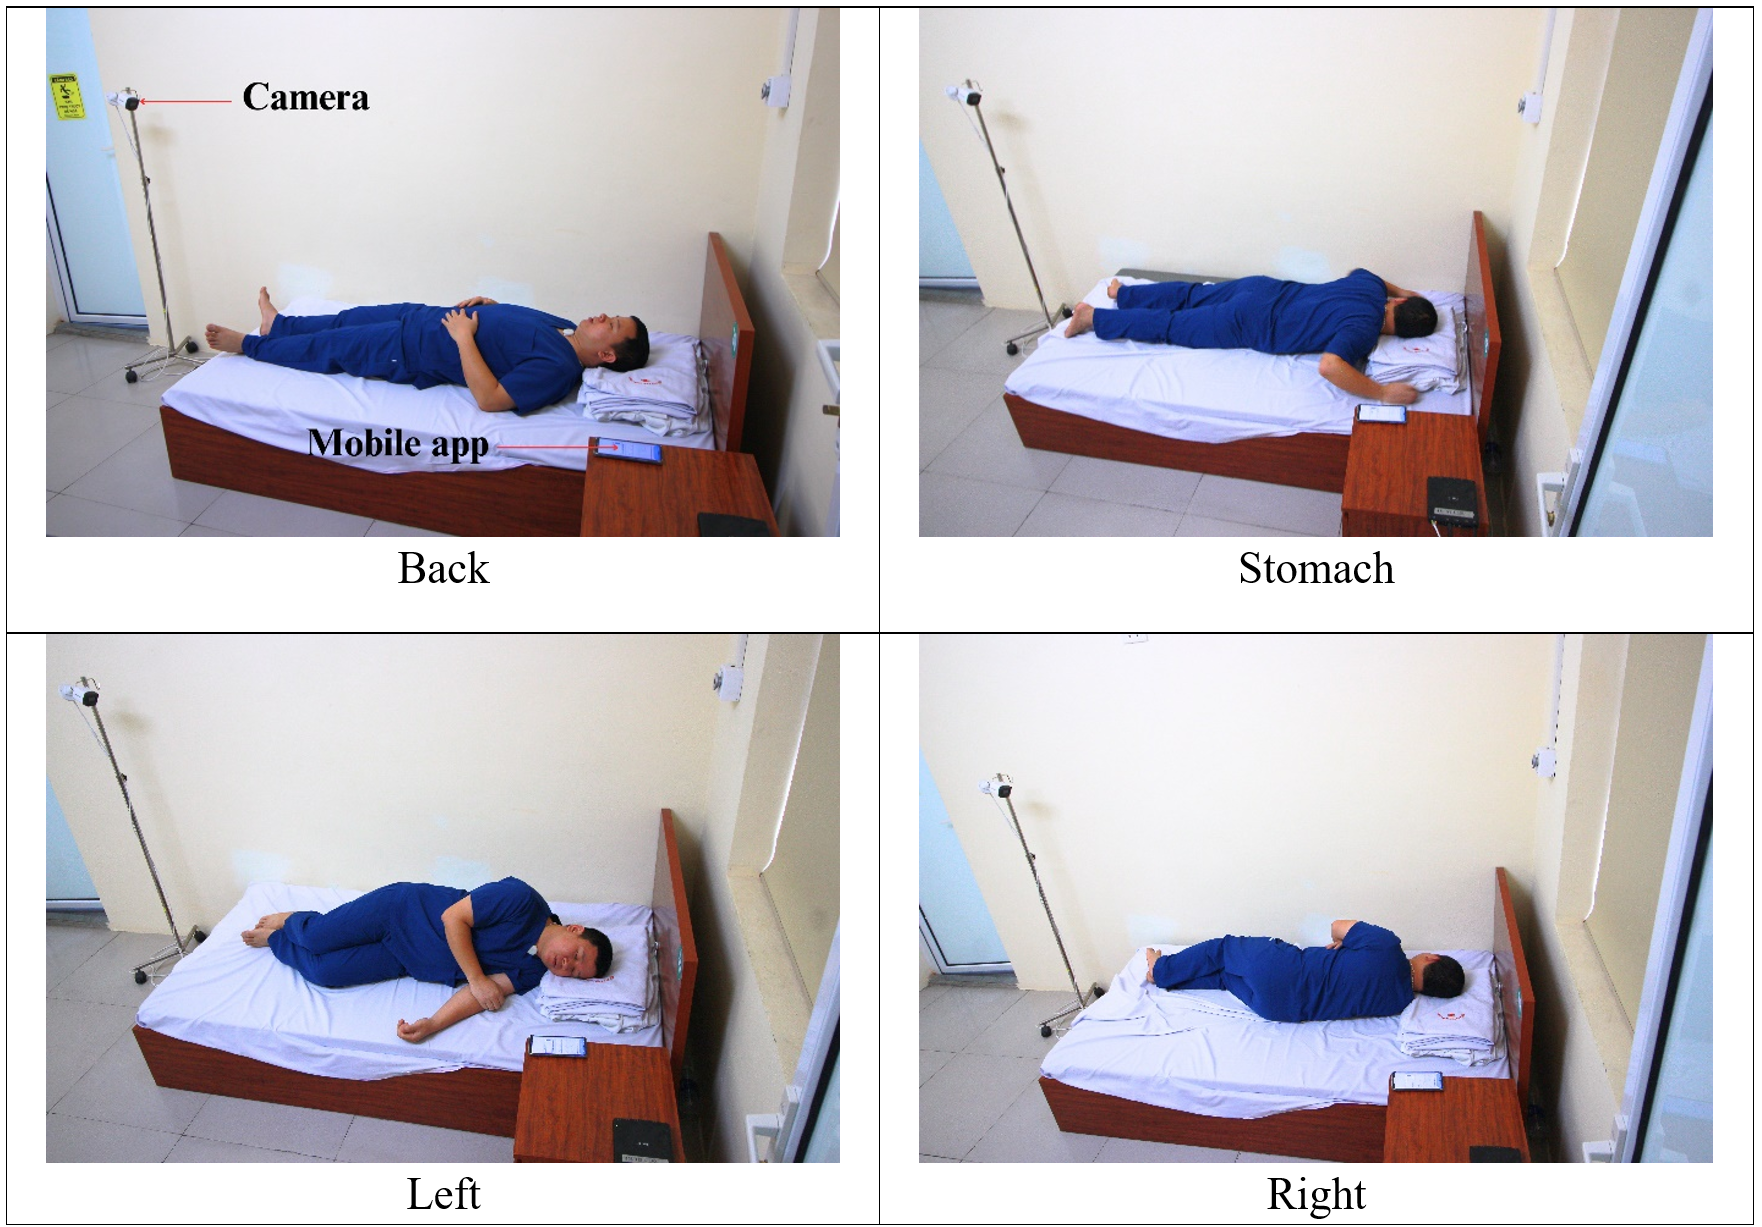
\includegraphics[width=0.8\linewidth]{images/4position.png}}
\caption{Mô phỏng thực nghiệm thực tế}
\label{4Position}
\end{figure}

Trong phần này, tác giả trình bày chi tiết phương pháp thu thập dữ liệu, 
các kịch bản thực nghiệm, cũng như quy trình xử lý và trích xuất đặc trưng 
để phục vụ cho việc huấn luyện các mô hình học máy trong bài toán nhận diện tư thế ngủ.

Tổng cộng 25 tình nguyện viên đã được tuyển chọn tham gia vào quá trình 
thu thập dữ liệu, với độ tuổi dao động từ 10 đến 60, trong đó độ tuổi 
phổ biến là 24. Nhóm tình nguyện viên bao gồm cả nam và nữ, được lựa 
chọn với tiêu chí đa dạng về giới tính và độ tuổi nhằm tăng tính đại 
diện và khách quan cho bộ dữ liệu.

Trong kịch bản đầu tiên (gọi là \textbf{thu thập có giám sát}), 
mỗi tình nguyện viên được hướng dẫn gắn thiết bị cảm biến vào vùng 
xương ức (ngay dưới hõm cổ) bằng băng keo y tế hai mặt 3M, 
sau đó đăng nhập vào ứng dụng di động với tài khoản cá nhân đã đăng ký. 
Dưới sự giám sát trực tiếp của tác giả, mỗi người tham gia sẽ lần 
lượt thực hiện các tư thế ngủ cơ bản (nằm ngửa, nằm sấp, nghiêng trái, nghiêng phải) 
trong thời gian tối thiểu 5 phút cho mỗi tư thế. 
Thứ tự thay đổi tư thế được thực hiện ngẫu nhiên nhằm tránh thiên 
lệch theo trình tự. Mỗi tư thế được lặp lại ít nhất hai lần để đảm 
bảo tính lặp lại và ổn định của tín hiệu.
Sau khi xác minh rằng dữ liệu cảm biến đã được lưu trữ đầy đủ 
trên hệ thống (kiểm tra trên MongoDB và giao diện ứng dụng), quá trình 
thu thập dữ liệu từ một tình nguyện viên được xem là hoàn tất.

Bên cạnh đó, để mô phỏng điều kiện thực tế khi sử dụng thiết bị trong 
sinh hoạt ban đêm, tác giả đã tự thực hiện kịch bản thứ hai 
(\textbf{thu thập trong giấc ngủ tự nhiên}). Trong kịch bản này, 
thiết bị được gắn vào cổ trước khi đi ngủ và ghi nhận dữ liệu liên 
tục trong suốt một đêm. Song song đó, một camera cố định được lắp 
đặt phía trên giường để ghi hình toàn bộ quá trình ngủ, từ đó hỗ 
trợ gán nhãn chính xác theo thời gian thực. Dữ liệu trong giai đoạn 
này được xử lý và đồng bộ thủ công giữa tín hiệu cảm biến và video 
để loại bỏ các đoạn có chuyển động hoặc sai lệch nhãn Hình~\ref{4Position}.

Mặc dù phương pháp thu thập trong môi trường tự nhiên sát với điều kiện 
sử dụng thực tế, nhưng đòi hỏi nhiều công sức xử lý hậu kỳ và 
khó kiểm soát chất lượng dữ liệu đầu vào. 
Theo ý kiến tư vấn từ các chuyên gia trong lĩnh vực y học giấc ngủ, 
phương pháp thu thập có giám sát (phương pháp 1) vẫn được ưu tiên do 
khả năng kiểm soát tốt, đảm bảo dữ liệu cân bằng giữa các tư thế, 
đồng thời vẫn duy trì được mức độ tương thích cao với điều kiện 
thực tế khi triển khai ứng dụng theo dõi tại nhà.

Sau quá trình thu thập, bộ dữ liệu huấn luyện bao gồm tổng cộng \textbf{158.750 mẫu} 
hợp lệ sau khi đã lọc nhiễu và loại bỏ các phiên ghi nhận không đạt yêu cầu của 25 tình nguyện viên. 
Dữ liệu kiểm thử sẽ là dữ liệu trong suốt một đêm ngủ tự nhiên của tác giả 
Việc gán nhãn dữ liệu được thực hiện thủ công bằng cách đồng bộ thời gian giữa 
tín hiệu cảm biến và dữ liệu video, sau đó loại bỏ toàn bộ các đoạn có chuyển động 
hoặc tư thế không rõ ràng. Kết quả là bộ dữ liệu kiểm thử gồm \textbf{64.258 mẫu} 
đảm bảo độ chính xác cao về mặt nhãn.

Tất cả dữ liệu thu thập từ các tình nguyện viên và tác giả đều được xuất ra định 
dạng \texttt{CSV}, bao gồm thông tin thời gian (timestamp), 
giá trị cảm biến trên ba trục $x$, $y$, $z$, và nhãn tư thế tương ứng 
(nếu có). Dữ liệu này được sử dụng làm đầu vào cho quá trình trích 
xuất đặc trưng và huấn luyện mô hình học máy.


\section{Phân loại tư thế ngủ bằng học máy}

\subsection{Phân tích dữ liệu}
Tư thế ngủ ban đầu có thể được ước lượng bằng phương pháp dựa trên ngưỡng 
(threshold-based), áp dụng trực tiếp lên dữ liệu cảm biến gia tốc ba 
trục. Trong phương pháp này, các ngưỡng được thiết lập trước cho từng 
trục ($x$, $y$, $z$), và sự thay đổi tư thế được suy đoán khi giá trị 
gia tốc đo được vượt quá ngưỡng tương ứng. Kỹ thuật này có ưu điểm là 
đơn giản, chi phí tính toán thấp, và đặc biệt phù hợp với các hệ thống 
nhúng tiêu thụ năng lượng thấp. 
Mặc dù kỹ thuật dựa trên ngưỡng có ưu điểm đơn giản và phù hợp với 
các hệ thống nhúng có tài nguyên hạn chế, nó tồn tại một số hạn chế 
nhất định. Cụ thể, phương pháp này khó phát hiện các chuyển động nhẹ 
hoặc tư thế trung gian giữa các trạng thái rõ ràng. Ngoài ra, các 
ngưỡng thường cần hiệu chỉnh theo từng cá nhân do sự khác biệt về 
hình thể, kiểu vận động và vị trí gắn cảm biến.


\begin{figure}[htbp]
\centering
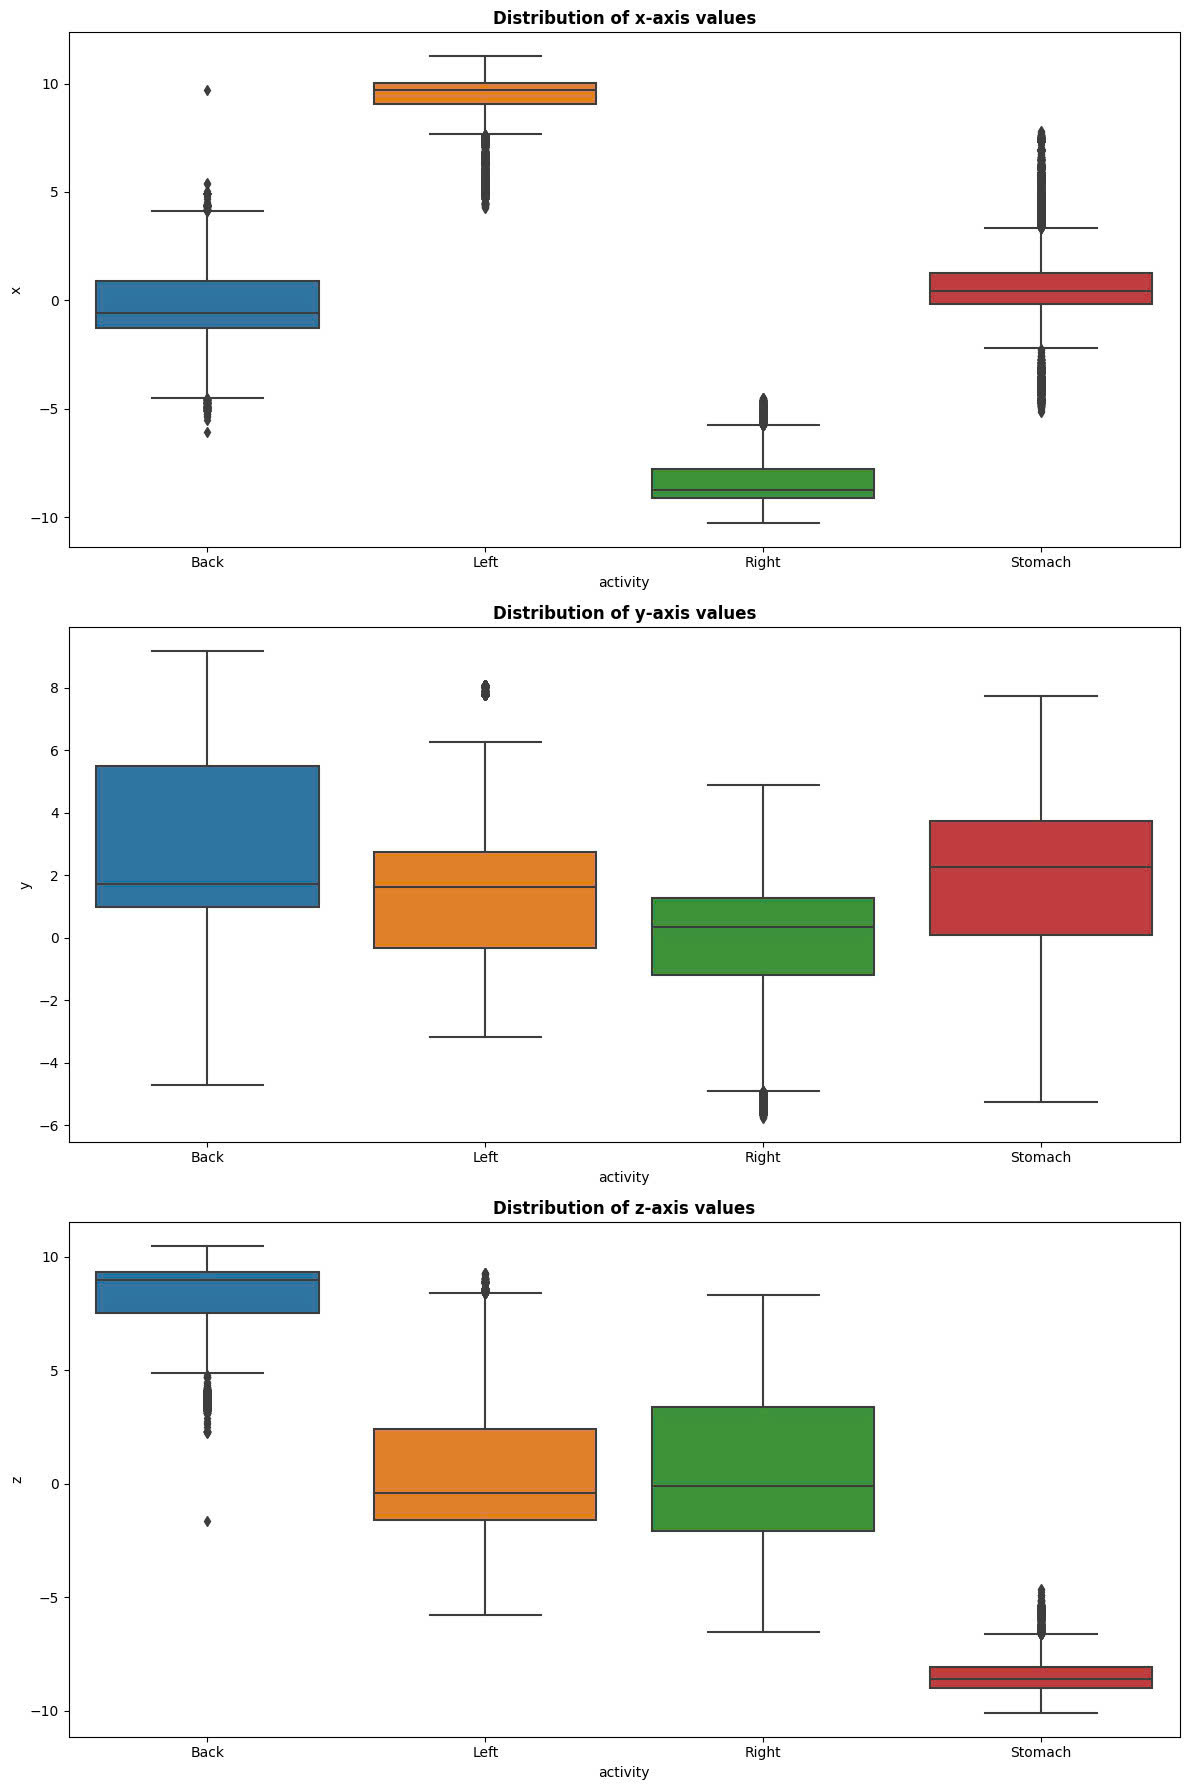
\includegraphics[width=0.7\linewidth]{images/threshhold.jpg} 
\caption{Phân bố dữ liệu cảm biến theo ba trục $x$, $y$, $z$ ứng với các tư thế ngủ khác nhau.}
\label{fig:axis_distribution}
\end{figure}
Hình~\ref{fig:axis_distribution} trình bày phân tích chi tiết phân bố 
tín hiệu cảm biến theo ba trục gia tốc ứng với bốn tư thế ngủ cơ bản. 
Ở trục $x$, các phân bố tương đối biệt lập, đặc biệt giữa hai tư thế 
nằm ngửa và nằm sấp, cũng như giữa nghiêng trái và nghiêng phải. 
Điều này cho thấy trục $x$ có khả năng phân biệt tư thế tốt. 
Ngược lại, trục $y$ thể hiện mức độ chồng lấn lớn giữa các tư thế, 
dẫn đến khả năng tách biệt thấp và ít giá trị trong việc xác định tư 
thế ngủ. Đối với trục $z$, có thể quan sát được sự phân tách 
rõ ràng giữa tư thế nằm nghiêng và các tư thế dọc 
(nằm ngửa và nằm sấp), chứng tỏ vai trò quan trọng của trục $z$ 
trong phân loại tư thế.



\begin{figure}[htbp]
\centering
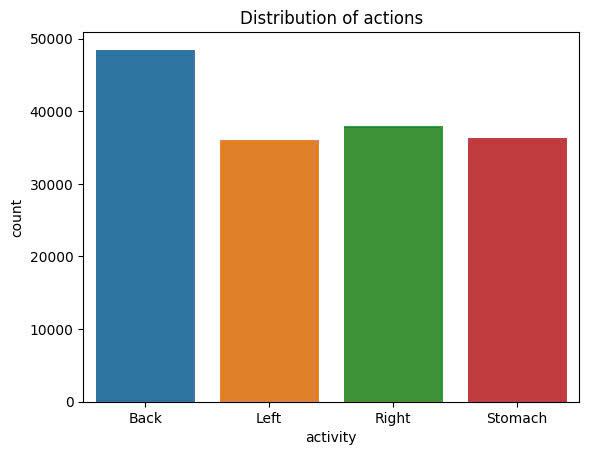
\includegraphics[width=0.6\linewidth]{images/distribution actions.jpg} 
\caption{Phân bố số lượng mẫu trong tập huấn luyện theo từng tư thế.}
\label{fig:countActions}
\end{figure}


Hình~\ref{fig:countActions} minh họa sự phân bố số lượng mẫu trong 
tập huấn luyện theo từng tư thế. Tư thế nằm ngửa (Back) chiếm tỷ 
trọng cao nhất với khoảng 50.000 mẫu, trong khi ba tư thế còn lại 
(nghiêng trái, nghiêng phải và nằm sấp) có số lượng tương đối cân bằng, 
dao động từ 30.000 đến 35.000 mẫu. Phân bố này phản ánh xu hướng phổ 
biến của tư thế nằm ngửa trong giấc ngủ tự nhiên, đồng thời cho thấy 
tầm quan trọng lâm sàng của tư thế này, đặc biệt trong bối cảnh hội 
chứng ngưng thở khi ngủ (OSA), khi tư thế nằm ngửa có thể làm trầm 
trọng tình trạng bệnh.



\subsection{Xử lý và trích xuất đặc trưng}

Dữ liệu cảm biến thu thập được trước tiên được xử lý khử nhiễu bằng 
phương pháp hiệu chỉnh điểm gốc (differential technique), bằng cách 
lấy hiệu giữa giá trị hiện tại và giá trị tham chiếu ban đầu trên ba 
trục $x$, $y$, và $z$. Sau đó, tín hiệu được chia thành các cửa sổ 
thời gian có độ dài 2 giây, với mức chồng lấn 50\% giữa các cửa sổ 
liên tiếp nhằm tăng độ mịn của chuỗi dữ liệu đầu vào.
Chỉ những cửa sổ dữ liệu có nhãn nhất quán trong toàn bộ thời gian 
mới được giữ lại để huấn luyện mô hình. Các cửa sổ chứa nhãn không 
đồng nhất (nhiều hơn một nhãn) hoặc có biểu hiện chuyển động bất 
thường sẽ bị loại bỏ khỏi quá trình xử lý tiếp theo.

\begin{table}[htbp]
\caption{Các đặc trưng thống kê và tín hiệu được sử dụng trong phân loại tư thế ngủ}
\label{tab:features}
\begin{center}
\renewcommand{\arraystretch}{1.5}
\begin{tabular}{|l|p{9.5cm}|}
\hline
\textbf{Đặc trưng} & \textbf{Mô tả / Công thức} \\
\hline
Giá trị trung bình & $\mu_s = \frac{1}{n} \sum_{i=1}^{n} S_i$ \\
\hline
Độ lệch chuẩn & $\sigma_s = \sqrt{\frac{1}{n} \sum_{i=1}^{n} (S_i - \mu_s)^2}$ \\
\hline
Độ lệch tuyệt đối trung bình & $\text{AAD} = \frac{1}{n} \sum_{i=1}^{n} |S_i - \mu_s|$ \\
\hline
Giá trị nhỏ nhất & $\min(s) = \min(S_1, S_2, \ldots, S_n)$ \\
\hline
Giá trị lớn nhất & $\max(s) = \max(S_1, S_2, \ldots, S_n)$ \\
\hline
Hiệu số lớn nhất - nhỏ nhất & $\max(s) - \min(s)$ \\
\hline
Trung vị & $\text{Median}(s) = \text{median}(S_1, S_2, \ldots, S_n)$ \\
\hline
Độ lệch tuyệt đối trung vị & $\text{MAD} = \frac{1}{n} \sum_{i=1}^{n} |S_i - \text{Median}(s)|$ \\
\hline
Khoảng tứ phân vị & $IQR = \text{percentile}(75) - \text{percentile}(25)$ \\
\hline
Số giá trị âm & $\#(S_i < 0)$ \\
\hline
Số giá trị dương & $\#(S_i > 0)$ \\
\hline
Số giá trị lớn hơn trung bình & $\#(S_i > \mu_s)$ \\
\hline
Số đỉnh (local maxima) & Số lượng điểm cực đại cục bộ trong chuỗi tín hiệu \\
\hline
Độ lệch (Skewness) & $\frac{1}{n \sigma_s^3} \sum_{i=1}^{n} (S_i - \mu_s)^3$ \\
\hline
Độ nhọn (Kurtosis) & $\frac{1}{n \sigma_s^4} \sum_{i=1}^{n} (S_i - \mu_s)^4$ \\
\hline
Năng lượng tín hiệu & $\sum_{i=1}^{n} S_i^2$ \\
\hline
Gia tốc tổng hợp trung bình & $\frac{1}{n} \sum_{i=1}^{n} \sqrt{x_i^2 + y_i^2 + z_i^2}$ \\
\hline
Tổng độ lớn tín hiệu (SMA) & $\frac{1}{n} \sum_{i=1}^{n} (|x_i| + |y_i| + |z_i|)$ \\
\hline
\end{tabular}
\end{center}
\end{table}

\subsubsection{Đặc trưng miền thời gian (T1)}\label{AA}

Dữ liệu cảm biến gia tốc vốn là chuỗi thời gian, do đó các đặc trưng miền thời gian đóng vai trò rất quan trọng trong nhận diện tư thế ngủ. Trong nghiên cứu này, tác giả trích xuất tổng cộng 40 đặc trưng thống kê cho mỗi cửa sổ dữ liệu, trên cả ba trục $x$, $y$, $z$. Các đặc trưng bao gồm giá trị trung bình, độ lệch chuẩn, độ lệch tuyệt đối trung bình, giá trị lớn nhất, nhỏ nhất, hiệu số lớn-nhỏ nhất, trung vị, độ lệch tuyệt đối trung vị, khoảng tứ phân vị, số lượng giá trị âm/dương, số lượng giá trị lớn hơn trung bình, số đỉnh tín hiệu, độ lệch, độ nhọn, năng lượng tín hiệu, gia tốc tổng hợp và tổng độ lớn tín hiệu. Các đặc trưng này được lựa chọn dựa trên tính dễ tính toán, hiệu quả phân tách tư thế và khả năng triển khai trên vi điều khiển.

\subsubsection{Đặc trưng miền tần số (F1)}\label{AA}

Để khai thác thông tin trong miền tần số, tác giả sử dụng Biến đổi Fourier Nhanh (FFT) để chuyển đổi dữ liệu từ miền thời gian sang miền tần số. Từ các cửa sổ tín hiệu sau biến đổi, 29 đặc trưng thống kê được tính toán, bao gồm các đặc trưng tương tự như trong miền thời gian: trung bình, độ lệch chuẩn, độ lệch tuyệt đối, giá trị cực đại – cực tiểu, trung vị, khoảng tứ phân vị, số đỉnh, độ lệch, độ nhọn, năng lượng tín hiệu,... Ngoài ra, hai đặc trưng kết hợp là gia tốc tổng hợp trung bình và tổng độ lớn tín hiệu (SMA) cũng được duy trì trong miền tần số để phục vụ so sánh với miền thời gian.

Việc sử dụng đồng thời các đặc trưng từ cả hai miền thời gian và tần số giúp tăng khả năng mô tả đặc trưng cho mô hình học máy, từ đó nâng cao hiệu quả phân loại tư thế ngủ trong các điều kiện khác nhau.

\subsection{Kịch bản kiểm thử và lựa chọn tính năng}

Lựa chọn đặc trưng là một bước quan trọng trong quá trình xây dựng mô hình học máy, giúp giảm chiều dữ liệu, cải thiện hiệu quả huấn luyện, rút ngắn thời gian tính toán và hạn chế hiện tượng quá khớp (overfitting). Nguyên lý chung là các đặc trưng hiệu quả phải có mối tương quan cao với biến mục tiêu (tư thế ngủ), đồng thời có mức tương quan thấp với nhau nhằm tránh dư thừa thông tin.

\textbf{Thứ nhất}, phân tích ma trận tương quan Pearson (Hình~\ref{fig:correlation}) đã cho thấy một số cặp đặc trưng có mức tương quan rất cao, điển hình như $x_{\mathrm{std}}$ và $x_{\mathrm{aad}}$ ($r = 0.98$), hay $y_{\mathrm{std}}$ và $y_{\mathrm{aad}}$ ($r = 0.68$). Điều này gợi ý rằng có thể loại bỏ một phần các đặc trưng trùng lặp nhằm giảm độ phức tạp mô hình mà vẫn giữ được thông tin cốt lõi.

\begin{figure}[htbp]
\centering
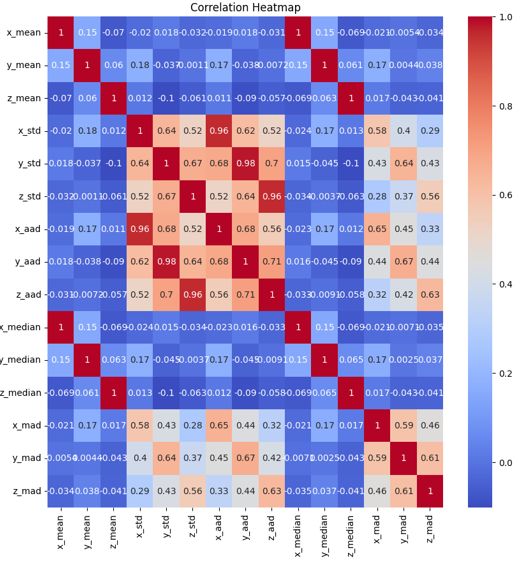
\includegraphics[width=1\linewidth]{images/correlation.png} 
\caption{Ma trận tương quan giữa các đặc trưng trích xuất. Cường độ màu thể hiện hệ số tương quan Pearson. Màu đỏ là tương quan dương mạnh, xanh là tương quan âm mạnh, xám là không tương quan.}
\label{fig:correlation}
\end{figure}

\textbf{Thứ hai}, kết quả phân tích SHAP (SHapley Additive exPlanations) ở Hình~\ref{fig:shap} chỉ ra rằng một số đặc trưng – đặc biệt là các đặc trưng miền thời gian trên trục $z$ như trung bình, năng lượng, trung vị – có ảnh hưởng vượt trội đến dự đoán của mô hình. Do đó, việc ưu tiên các đặc trưng này trong kịch bản triển khai nhẹ (TinyML) là hoàn toàn hợp lý về mặt kỹ thuật.

\begin{figure}[htbp]
\centering
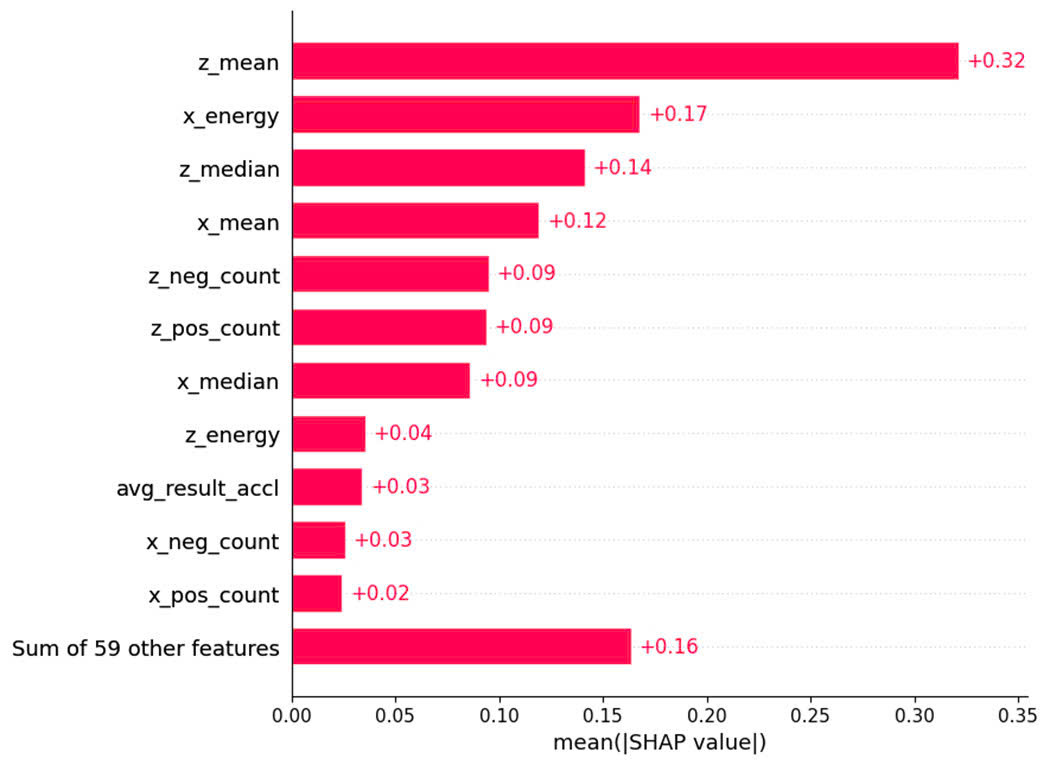
\includegraphics[width=0.8\linewidth]{images/shap20.jpg} 
\caption{Phân tích giá trị SHAP nhằm xác định tầm quan trọng của các đặc trưng trong mô hình phân loại tư thế ngủ. Các đặc trưng từ trục $z$ chiếm ưu thế về mức ảnh hưởng đến đầu ra mô hình.}
\label{fig:shap}
\end{figure}

\textbf{Thứ ba}, để hệ thống hóa việc đánh giá vai trò của từng nhóm đặc trưng và cấu hình mô hình, tác giả đã xây dựng tám kịch bản thực nghiệm được trình bày trong Bảng~\ref{tab:scenarios}. Các kịch bản được thiết kế nhằm phản ánh đầy đủ các yếu tố cần đánh giá như loại đặc trưng (miền thời gian, tần số), mức độ tương quan, độ dài cửa sổ tín hiệu và bộ đặc trưng tối ưu hoá bằng SHAP.

\begin{table}[htbp]
\caption{Các kịch bản lựa chọn và sử dụng đặc trưng trong nghiên cứu}
\label{tab:scenarios}
\begin{center}
\renewcommand{\arraystretch}{1.2}
\begin{tabular}{|c|p{6.1cm}|}
\hline
\textbf{Kịch bản} & \textbf{Mô tả} \\
\hline
1 & Sử dụng toàn bộ đặc trưng để đánh giá ảnh hưởng tổng thể đến mô hình. \\
\hline
2 & Áp dụng toàn bộ đặc trưng trong miền thời gian. \\
\hline
3 & Áp dụng toàn bộ đặc trưng trong miền tần số. \\
\hline
4 & Sử dụng đặc trưng miền thời gian, loại bỏ các đặc trưng có tương quan $>$ 95\%. \\
\hline
5 & Chọn ra 11 đặc trưng quan trọng nhất theo giá trị SHAP. \\
\hline
6 & Dùng cửa sổ 3 giây (50\% overlap), với 11 đặc trưng SHAP. \\
\hline
7 & Dùng cửa sổ 1 giây (50\% overlap), với 11 đặc trưng SHAP. \\
\hline
8 & Dùng cửa sổ 2 giây (25\% overlap), với 11 đặc trưng SHAP. \\
\hline
\end{tabular}
\end{center}
\end{table}

Đối với các kịch bản 5 đến 8, việc lựa chọn 11 đặc trưng được thực hiện bằng cách huấn luyện mô hình Random Forest trên toàn bộ tập đặc trưng, sau đó tính giá trị SHAP trung bình cho từng đặc trưng và chọn ra nhóm có ảnh hưởng cao nhất. Việc rút gọn đặc trưng này giúp mô hình nhẹ hơn, nhanh hơn, phù hợp với môi trường nhúng có giới hạn về bộ nhớ và tính toán.

Các kịch bản 6 đến 8 thay đổi độ dài cửa sổ trượt (1 giây, 2 giây, 3 giây) và mức chồng lấn nhằm khảo sát tác động của kích thước đoạn tín hiệu đến hiệu quả mô hình, đồng thời phản ánh điều kiện sử dụng thực tế trong các thiết bị đeo (wearables) hoặc hệ thống biên (edge-AI).

Với thiết kế kịch bản như trên, luận văn không chỉ đánh giá hiệu quả mô hình theo nhiều hướng khác nhau, mà còn hướng tới việc xác định cấu hình tối ưu giữa độ chính xác, chi phí tính toán và khả năng triển khai thực tiễn.

\subsection{Huấn luyện mô hình}

Dựa trên các phương pháp phân loại được đề cập ở các phần trước — 
bao gồm phương pháp ngưỡng, học máy và học sâu — 
tác giả đã lựa chọn một tập hợp đại diện các mô hình để 
tiến hành đánh giá hiệu quả trong bài toán nhận diện tư thế ngủ 
từ dữ liệu cảm biến gia tốc. Cụ thể, bốn mô hình học máy truyền 
thống được lựa chọn từ thư viện \texttt{scikit-learn} gồm: 
\textbf{Random Forest (RF)}, \textbf{Logistic Regression (LR)}, 
\textbf{Support Vector Machine (SVM)}, và \textbf{Gradient Boosting (GB)}. 
Đây đều là các mô hình đã được chứng minh hiệu quả trong việc xử lý dữ 
liệu cảm biến có cấu trúc, đặc biệt trong các bài toán phân loại đa lớp.

Để đảm bảo tính công bằng trong so sánh và khả năng triển khai thực tế trên vi điều khiển, các siêu tham số (hyperparameters) của từng mô hình được lựa chọn dựa trên kinh nghiệm thực tiễn trong các công trình trước và quá trình tinh chỉnh sơ bộ nhằm đạt được sự cân bằng giữa độ chính xác và độ phức tạp tính toán. Chi tiết tham số của từng mô hình được trình bày trong Bảng~\ref{tab:models}.

\begin{table}[htbp]
\caption{Các mô hình học máy và siêu tham số sử dụng trong nghiên cứu}
\label{tab:models}
\centering
\renewcommand{\arraystretch}{1.2}
\begin{tabular}{|l|p{9cm}|}
\hline
\textbf{Mô hình} & \textbf{Tham số cấu hình} \\
\hline
\textbf{Random Forest (RF)} & 
Số cây quyết định: 50; \newline
Độ sâu tối đa: 5; \newline
Số đặc trưng được xét tại mỗi nút: \texttt{log2} \\
\hline
\textbf{Logistic Regression (LR)} & 
Chiến lược đa lớp: \texttt{one-vs-rest}; \newline
Số vòng lặp tối đa: 50; \newline
Hàm tối ưu: \texttt{lbfgs} \\
\hline
\textbf{Support Vector Machine (SVM)} & 
Hàm kernel: \texttt{sigmoid}; \newline
Tham số điều chuẩn $C = 2$; \newline
Chiến lược đa lớp: \texttt{one-vs-rest} \\
\hline
\textbf{Gradient Boosting (GB)} & 
Tốc độ học: 0.01; \newline
Số lượng cây tăng cường: 50; \newline
Độ sâu tối đa: 3; \newline
Số đặc trưng được chọn: \texttt{log2} \\
\hline
\textbf{Mạng nơ-ron (Neural Network, Keras)} & 
Cấu trúc: [8, 4, \textit{num\_classes}]; \newline
Hàm kích hoạt: \texttt{ReLU}, \texttt{ReLU}, \texttt{Softmax}; \newline
Thuật toán tối ưu: \texttt{Adam} (learning rate = 0.01); \newline
Hàm mất mát: \texttt{sparse\_categorical\_crossentropy}; \newline
Độ đo đánh giá: \texttt{accuracy} \\
\hline
\end{tabular}
\end{table}

Ngoài các mô hình học máy, một mạng nơ-ron nhân tạo tuyến tính đơn giản 
(feedforward neural network) được xây dựng bằng thư viện \texttt{TensorFlow/Keras} 
để đại diện cho phương pháp học sâu. 
Mạng bao gồm hai lớp ẩn với số lượng nơ-ron lần lượt là 8 và 4, 
theo sau là một lớp đầu ra sử dụng hàm kích hoạt \texttt{Softmax} cho bài toán phân loại đa lớp. 
Các lớp ẩn sử dụng hàm kích hoạt \texttt{ReLU} nhằm mô hình hóa các quan hệ phi tuyến hiệu quả hơn. 
Mô hình này được tối ưu bằng thuật toán \texttt{Adam} với tốc độ học (learning rate) là 0.01 
và được huấn luyện bằng hàm mất mát \texttt{sparse\_categorical\_crossentropy}, 
sử dụng độ đo đánh giá \texttt{accuracy} để phản ánh hiệu suất phân loại.

Việc lựa chọn kết hợp các mô hình với mức độ phức tạp khác nhau cho phép đánh giá toàn diện về 
hiệu quả phân loại trong các điều kiện thực tế. 
Từ các mô hình cây đơn giản và dễ diễn giải, đến các mô hình mạnh 
hơn như Gradient Boosting hoặc mạng nơ-ron – nghiên cứu nhằm tìm r
a giải pháp cân bằng tối ưu giữa độ chính xác, kích thước mô hình, 
tốc độ suy luận (inference latency) và mức sử dụng bộ nhớ, 
phục vụ cho các ứng dụng thực tiễn như hệ thống AI biên (Edge-AI) 
hoặc thiết bị đeo thông minh.
\subsection{Đánh giá kết quả}
Để đánh giá hiệu quả của các mô hình học máy và tác động của lựa 
chọn đặc trưng đầu vào, tám kịch bản thực nghiệm đã được thiết kế 
như trình bày ở các phần trước. Các kịch bản này không chỉ cho phép 
phân tích ảnh hưởng của đặc trưng, cửa sổ tín hiệu và trục cảm biến, 
mà còn hướng đến tối ưu hóa trọng số mô hình phục vụ triển khai trên 
thiết bị nhúng.


\begin{table}[htbp]
\caption{Độ chính xác phân loại của các mô hình trong 8 kịch bản}
\label{tab:accuracy}
\centering
\renewcommand{\arraystretch}{1.1}
\scriptsize
\begin{tabular}{|l|c|c|c|c|c|c|c|c|}
\hline
\textbf{Mô hình} & S1 & S2 & S3 & S4 & S5 & S6 & S7 & S8 \\
\hline
LR  & 0.970 & 0.970 & 0.368 & 0.970 & 0.987 & 0.990 & 0.990 & 0.987 \\
RF  & 0.995 & 0.996 & 0.426 & 0.994 & 0.993 & 0.993 & 0.993 & 0.991 \\
SVM & 0.995 & 0.985 & 0.280 & 0.991 & 0.989 & 0.982 & 0.982 & 0.870 \\
GB  & 0.996 & 0.996 & 0.439 & 0.995 & 0.995 & 0.996 & 0.996 & 0.996 \\
NN  &  0.920 &  --   &  --   &  --   &  --   &  --   &  --   & -- \\
\hline
\end{tabular}
\end{table}

Kết quả trong Bảng~\ref{tab:accuracy} làm sáng tỏ sự khác biệt căn bản giữa các nhóm đặc trưng và cách tiếp cận mô hình. 
Trước hết, \textbf{Gradient Boosting (GB)} nổi bật với hiệu năng ổn định nhất, 
liên tục đạt giá trị chính xác tối đa (0.996) trong năm kịch bản (S1, S2, S6, S7, S8). 
Đặc điểm này cho thấy ưu thế vượt trội của các phương pháp tăng cường mô hình dựa trên cây quyết định, 
khả năng khai thác tốt cả quan hệ phi tuyến và sự tương tác giữa các đặc trưng. 
\textbf{Random Forest (RF)} mặc dù có đôi chút biến thiên, nhưng vẫn duy trì độ chính xác vượt ngưỡng 0.99 trong hầu hết kịch bản, 
củng cố vai trò của các mô hình ensemble dựa trên bootstrap aggregation trong việc giảm phương sai và cải thiện khả năng tổng quát hoá.  

Trái lại, \textbf{Logistic Regression (LR)} và \textbf{Support Vector Machine (SVM)} 
chỉ đạt được hiệu năng tiệm cận 0.99 trong các kịch bản sử dụng đặc trưng miền thời gian hoặc đặc trưng được lựa chọn bằng SHAP. 
Đặc biệt, ở kịch bản S3 – vốn chỉ khai thác đặc trưng miền tần số – cả hai mô hình này sụt giảm nghiêm trọng về độ chính xác (LR còn 0.368, SVM chỉ 0.280). 
Kết quả nhấn mạnh rằng các tín hiệu động học quan trọng để phân loại chủ yếu được mã hoá trong miền thời gian. 
Điều này hoàn toàn tương thích với phân tích SHAP (Hình~\ref{fig:shap}), 
khi các đặc trưng đóng góp nhiều nhất đều tập trung ở miền thời gian, đặc biệt trên trục $z$, 
nơi thể hiện rõ sự khác biệt về động học tư thế.

Một điểm đáng chú ý khác là khi áp dụng cơ chế chọn lọc đặc trưng dựa trên \textbf{SHAP} (các kịch bản S5–S8), 
độ chính xác của các mô hình hầu như không suy giảm, thậm chí trong một số trường hợp còn được cải thiện nhẹ 
(ví dụ LR đạt 0.990 ở S6 và S7 so với 0.970 ở S1). 
Điều này chứng tỏ việc loại bỏ các đặc trưng dư thừa và tập trung vào những đặc trưng quan trọng nhất 
không chỉ giúp giảm chiều dữ liệu mà còn hạn chế hiện tượng nhiễu, từ đó gia tăng độ khái quát hoá. 
Kết quả này có ý nghĩa thực tiễn quan trọng, vì nó cho phép duy trì hiệu năng phân loại cao 
trong khi giảm thiểu chi phí tính toán và bộ nhớ – yếu tố then chốt khi triển khai trên các thiết bị nhúng hoặc hệ thống IoT có tài nguyên hạn chế.

Tóm lại, Bảng~\ref{tab:accuracy} không chỉ xác nhận ưu thế vượt trội của các mô hình ensemble như GB và RF, 
mà còn chứng minh tính hiệu quả của phương pháp chọn lọc đặc trưng dựa trên SHAP. 
Sự thất bại rõ rệt của kịch bản S3 nhấn mạnh rằng miền tần số không mang lại giá trị phân loại đáng kể trong trường hợp này, 
trong khi các đặc trưng miền thời gian mới là nguồn thông tin then chốt để mô hình học được ranh giới phân lớp một cách chính xác và bền vững.




\begin{figure}[htbp]
    \centering
    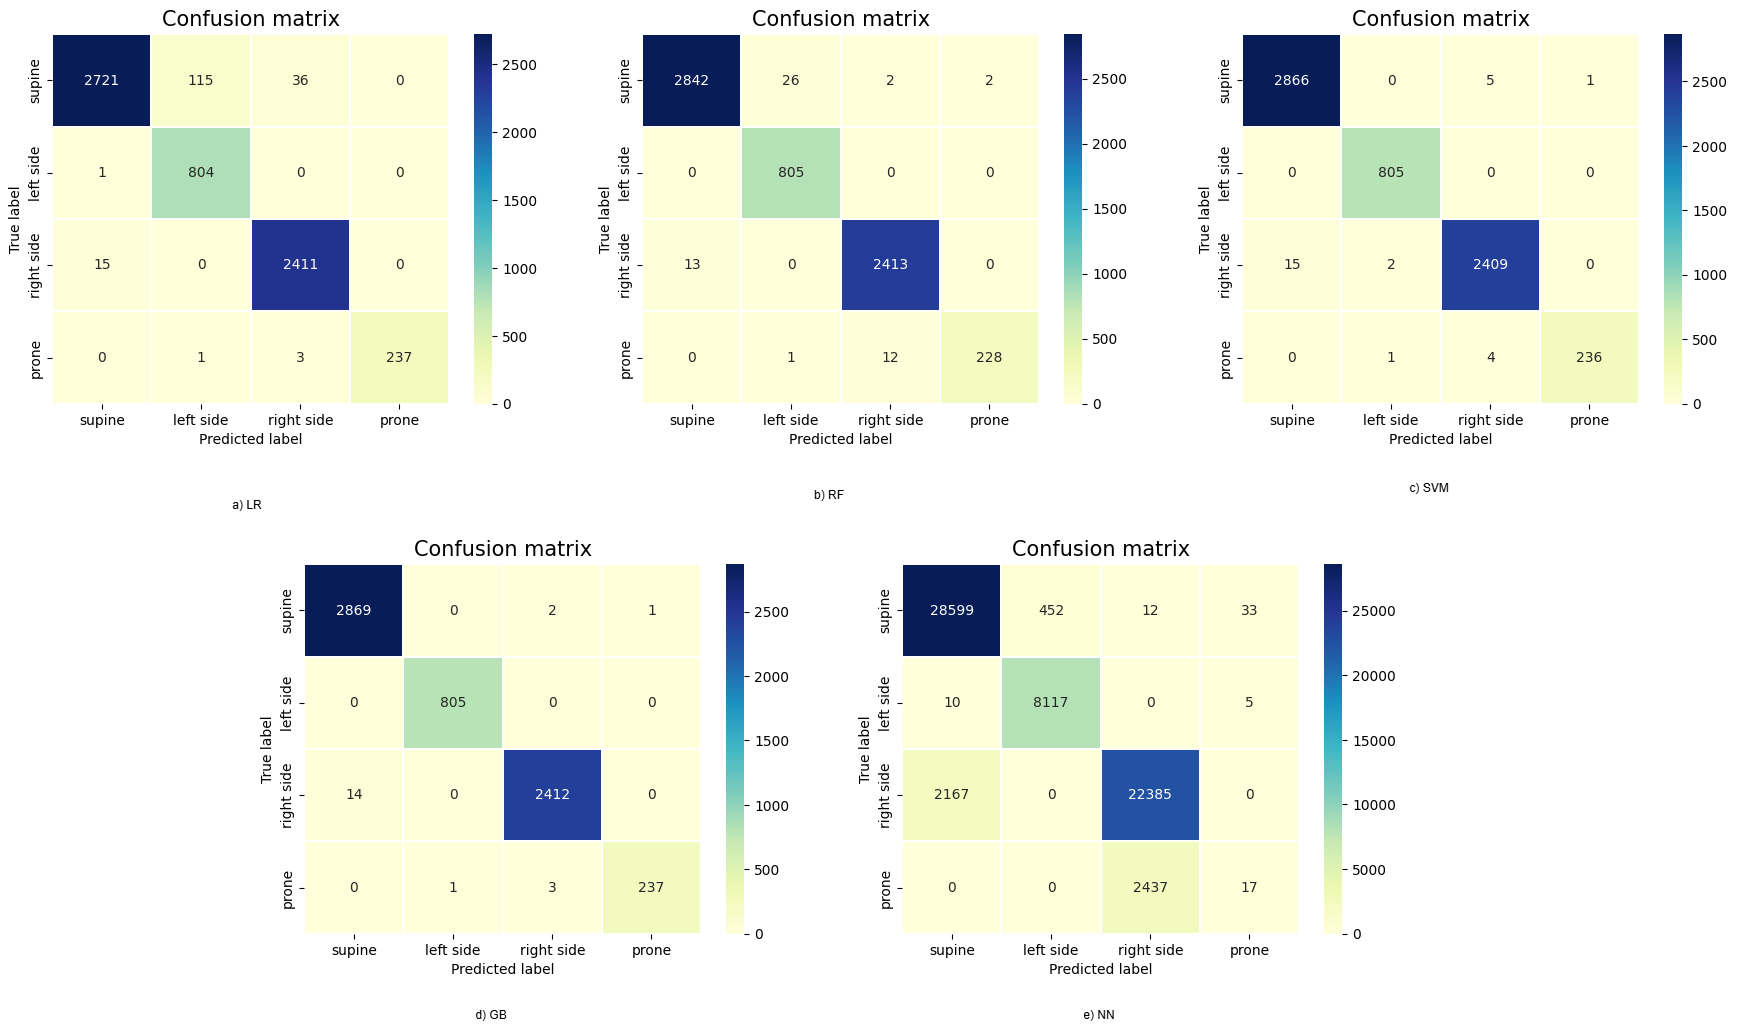
\includegraphics[width=\linewidth]{images/matrix (2).png}
    \caption{Ma trận nhầm lẫn (confusion matrix) của năm mô hình 
    phân loại trong kịch bản S1. GB và RF cho kết quả chính xác 
    cao nhất. Mô hình NN được huấn luyện trực tiếp trên dữ liệu thô.}
    \label{fig:cm_all_models}
\end{figure}

Kết quả này nhấn mạnh vai trò then chốt của lựa chọn đặc trưng đầu vào đối với hiệu quả mô hình. Các kịch bản sử dụng đặc trưng đã rút gọn theo SHAP (như S5–S8) vừa đạt độ chính xác cao, vừa giảm số chiều dữ liệu đầu vào, qua đó hỗ trợ triển khai mô hình nhẹ trong môi trường nhúng. Ngược lại, các kịch bản thiếu chọn lọc như S3 dẫn đến hiệu suất kém.

\begin{table}[htbp]
\caption{Kích thước mô hình (KB) trong 8 kịch bản}
\label{tab:modelsize}
\centering
\renewcommand{\arraystretch}{1.1}
\scriptsize
\begin{tabular}{|l|c|c|c|c|c|c|c|c|}
\hline
\textbf{Mô hình} & S1 & S2 & S3 & S4 & S5 & S6 & S7 & S8 \\
\hline
LR  & 4   & 2   & 2    & 2   & 2   & 2   & 2   & 2   \\
RF  & 187 & 151 & 291  & 176 & 89  & 89  & 141 & 103 \\
SVM & 315 & 232 & 3051 & 294 & 150 & 92  & 183 & 274 \\
GB  & 605 & 602 & 615  & 603 & 587 & 587 & 587 & 589 \\
NN  & 55  & --  & --   & --  & --  & --  & --  & --   \\
\hline
\end{tabular}
\end{table}

Bảng~\ref{tab:modelsize} cho thấy sự khác biệt đáng kể về kích thước giữa các mô hình. 
\textbf{Gradient Boosting (GB)} luôn duy trì dung lượng trên 580~KB bất kể kịch bản, 
cho thấy tính ổn định nhưng đồng thời cũng phản ánh hạn chế khi triển khai trên thiết bị nhúng có bộ nhớ giới hạn. 
\textbf{Random Forest (RF)} có kích thước biến thiên rõ rệt (89–291~KB) phụ thuộc vào số lượng và loại đặc trưng đầu vào, 
song vẫn duy trì ở mức chấp nhận được đối với các nền tảng nhúng có tài nguyên trung bình.  

Ngược lại, \textbf{Logistic Regression (LR)} chỉ chiếm 2–4~KB, 
một dung lượng cực kỳ nhỏ, khiến mô hình này trở thành ứng viên lý tưởng trong các hệ thống vi điều khiển hoặc IoT cần tối ưu bộ nhớ, 
mặc dù độ chính xác có phần thấp hơn so với các mô hình ensemble. 
\textbf{Support Vector Machine (SVM)} thường dao động trong khoảng 92–315~KB, 
tuy nhiên ở kịch bản S3 kích thước tăng vọt lên 3051~KB, 
nguyên nhân xuất phát từ số chiều đầu vào lớn và cấu trúc bộ nhớ của kernel. 
Điều này cho thấy SVM kém ổn định về mặt tài nguyên và khó kiểm soát khi triển khai thực tế.  

Đáng chú ý, \textbf{Neural Network (NN)} ở kịch bản S1 đạt độ chính xác 0.92 với dung lượng chỉ 55~KB. 
Mặc dù chưa đạt hiệu năng tối ưu, kết quả này mở ra hướng tiếp cận tiềm năng cho các ứng dụng Edge AI, 
nơi sự cân bằng giữa hiệu năng và tính gọn nhẹ được đặt lên hàng đầu.  

Tổng thể, Bảng~\ref{tab:modelsize} nhấn mạnh bài toán đánh đổi (trade-off) giữa \emph{hiệu quả dự đoán} và \emph{tài nguyên triển khai}. 
Trong khi RF và GB cho kết quả phân loại vượt trội về độ chính xác, 
thì LR và NN lại nổi bật nhờ kích thước gọn nhẹ, đặc biệt phù hợp với môi trường hạn chế tài nguyên. 
Sự đánh đổi này cho thấy rằng lựa chọn mô hình tối ưu không chỉ dựa vào độ chính xác thuần tuý, 
mà còn phụ thuộc vào yêu cầu hệ thống và ngữ cảnh triển khai cụ thể.
Từ hai bảng kết quả có thể thấy rõ sự đánh đổi giữa \emph{hiệu năng phân loại} và \emph{tài nguyên triển khai}. 
Trong bối cảnh nghiên cứu hướng đến ứng dụng trên thiết bị nhúng và hệ thống IoT, 
các mô hình có kích thước gọn nhẹ nhưng vẫn duy trì độ chính xác ở mức cao cần được ưu tiên. 
Do đó, mặc dù \textbf{RF} và \textbf{GB} thể hiện hiệu năng vượt trội về mặt độ chính xác, 
luận án lựa chọn thử nghiệm chuyên sâu với \textbf{Logistic Regression (LR)} và \textbf{Neural Network (NN)}. 
Hai mô hình này có ưu điểm quan trọng: dung lượng bộ nhớ rất nhỏ (2--4~KB đối với LR, 55~KB đối với NN) 
và khả năng triển khai thuận lợi trên vi điều khiển, vốn thường chỉ có vài trăm kilobyte bộ nhớ khả dụng.  

Một điểm cần lưu ý là các kịch bản S1–S5 được xây dựng với cửa sổ trượt 2~giây, 
trong khi các kịch bản S7 sử dụng cửa sổ 1~giây với mức chồng lấn 50\%. 
Kết quả cho thấy việc giảm độ dài cửa sổ từ 2~giây xuống 1~giây không làm suy giảm đáng kể độ chính xác 
(thậm chí trong một số trường hợp, LR và GB còn cải thiện nhẹ, ví dụ LR đạt 0.990 ở S7 so với 0.987 ở S5). 
Việc lựa chọn cửa sổ 1~giây thay vì 2~giây có ý nghĩa thực tiễn quan trọng: 
nó cho phép hệ thống phản hồi nhanh hơn, nắm bắt kịp thời sự thay đổi tư thế, 
đồng thời giảm độ trễ trong nhận dạng – một yêu cầu thiết yếu khi triển khai trong môi trường y tế thực tế.  

Tóm lại, mặc dù các mô hình ensemble như RF và GB đạt hiệu năng cao nhất về mặt số liệu, 
luận án định hướng ưu tiên triển khai thử nghiệm với LR và NN kết hợp cửa sổ 1~giây. 
Đây là lựa chọn cân bằng hợp lý giữa \emph{độ chính xác}, \emph{tính gọn nhẹ của mô hình}, 
và \emph{khả năng đáp ứng thời gian thực} khi triển khai trong các hệ thống nhúng hỗ trợ giám sát sức khỏe.

\section{Triển khai trên vi điều khiển nhúng}

Sau khi hoàn tất quá trình huấn luyện và đánh giá trên máy tính, bước tiếp theo của nghiên cứu là kiểm chứng khả năng triển khai mô hình trong môi trường thực tế sử dụng vi điều khiển nhúng. Mục tiêu khoa học ở giai đoạn này không chỉ dừng ở việc “chạy được” mô hình trên phần cứng hạn chế, mà còn nhằm làm sáng tỏ mối quan hệ đánh đổi giữa hiệu năng thuật toán và giới hạn tài nguyên của hệ thống nhúng.  

Cụ thể, nghiên cứu tiến hành triển khai song song hai mô hình: mạng nơ-ron nông (Neural Network – NN) với khả năng biểu diễn phi tuyến mạnh mẽ, và hồi quy logistic (Logistic Regression – LR) với cấu trúc tuyến tính cực kỳ gọn nhẹ. NN được kỳ vọng duy trì độ chính xác cao trong phân loại tư thế ngủ, trong khi LR đóng vai trò như một đối chứng quan trọng, minh chứng cho khả năng đạt được sự cân bằng tối ưu giữa độ chính xác vừa đủ và mức tiêu thụ tài nguyên tối thiểu.  

Điều này cho thấy trong bối cảnh phần cứng hạn chế, giá trị khoa học không nằm ở việc đạt độ chính xác tuyệt đối trong điều kiện lý tưởng, mà ở khả năng thiết kế một mô hình “đủ tốt” nhưng có thể vận hành bền vững trên chip. Chính sự đánh đổi này khẳng định nguyên lý cốt lõi của TinyML: hy sinh một phần nhỏ về độ chính xác để đổi lấy tính khả thi, hiệu quả năng lượng và độ tin cậy trong môi trường thực.  

Kết quả cũng cho thấy sự song hành giữa hai mô hình được lựa chọn. Mạng nơ-ron (NN) duy trì độ chính xác cao nhưng tiêu tốn nhiều tài nguyên, trong khi hồi quy logistic (LR) có dung lượng siêu nhỏ, tốc độ suy luận nhanh, và vẫn giữ mức chính xác tiệm cận. Việc triển khai song song cả NN và LR trên chip vì vậy không chỉ mang ý nghĩa kiểm chứng kỹ thuật, mà còn cung cấp bằng chứng khoa học cho thấy ranh giới cân bằng giữa “độ chính xác tối đa” và “khả năng ứng dụng thực tế” trong hệ thống nhúng y sinh.


\subsection{Quy trình triển khai mô hình}


Dựa trên các kết quả phân tích và đánh giá ở giai đoạn~1, 
tác giả quyết định bước sang giai đoạn~2 với mục tiêu triển khai thực tế trên phần cứng nhúng. 
Như đã trình bày, hai mô hình được lựa chọn cho thử nghiệm là \textbf{Neural Network (NN)} 
và \textbf{Logistic Regression (LR)}, bởi chúng đáp ứng tốt yêu cầu về tính gọn nhẹ và khả năng triển khai trên vi điều khiển.  

Quy trình triển khai bao gồm các bước sau:  
\begin{enumerate}
    \item \textbf{Xác định vi điều khiển mục tiêu}: lựa chọn nền tảng phần cứng phù hợp với giới hạn bộ nhớ và khả năng tính toán.  
    \item \textbf{Thu thập lại dữ liệu trực tiếp trên vi điều khiển}: đảm bảo dữ liệu phản ánh đúng điều kiện hoạt động của phần cứng thực tế, tránh sai lệch do khác biệt môi trường so với giai đoạn mô phỏng.  
    \item \textbf{Huấn luyện lại mô hình}: sử dụng bộ dữ liệu thu thập mới để tinh chỉnh và tái huấn luyện, nhằm tối ưu hóa mô hình cho nền tảng phần cứng được chọn.  
    \item \textbf{Chuyển đổi mô hình sang mã C/C++}: áp dụng các công cụ biên dịch và chuyển đổi chuyên dụng để xuất mô hình dưới dạng mã nguồn có thể nhúng trực tiếp.  
    \item \textbf{Triển khai trên chip}: nạp mã nguồn vào vi điều khiển, kiểm tra khả năng suy luận và hiệu năng thời gian thực.  
\end{enumerate}
\subsubsection{B1}

Vi điều khiển được lựa chọn là \textbf{Arduino Nano 33 BLE Sense}, sử dụng chip \texttt{nRF52840} (ARM Cortex-M4F, 64~MHz), 1~MB flash và 256~KB RAM. Bo mạch này cũng tích hợp sẵn cảm biến gia tốc, rất phù hợp để xây dựng hệ thống nhận diện tư thế ngủ hoàn chỉnh và hoạt động độc lập.

\subsubsection{B2}

Qua nhiều lần triển khai thực nghiệm trực tiếp trên vi điều khiển, 
tác giả đã rút ra một kết luận quan trọng: 
việc \textbf{giảm số lượng mẫu huấn luyện} kết hợp với \textbf{rút gọn tập đặc trưng} 
mang lại hiệu quả rõ rệt trong việc tối ưu mô hình cho môi trường nhúng. 
Cụ thể, các mô hình sau khi được tinh giản có \emph{kích thước tệp nhỏ hơn}, 
\emph{mức sử dụng bộ nhớ giảm đáng kể}, và \emph{thời gian suy luận nhanh hơn}, 
nhưng độ chính xác chỉ suy giảm ở mức rất nhỏ và hoàn toàn nằm trong ngưỡng chấp nhận được đối với ứng dụng thực tế. 
Điều này chứng tỏ rằng, trong bối cảnh triển khai Edge AI, 
sự đánh đổi giữa số lượng đặc trưng và hiệu năng mô hình có thể được cân bằng một cách hợp lý, 
từ đó vừa đảm bảo tính khả thi trên phần cứng hạn chế, vừa duy trì độ tin cậy trong dự đoán.  

Đặc biệt, ở \textbf{bước 2 của quy trình}, tác giả đã tiến hành \emph{thu thập lại 1.470 mẫu dữ liệu} 
trực tiếp từ thiết bị \textbf{Arduino Nano 33 BLE Sense}. 
Khác với bộ dữ liệu mô phỏng trên máy tính, tập dữ liệu này phản ánh sát thực tế điều kiện hoạt động của phần cứng, 
bao gồm cả đặc điểm nhiễu, độ trễ và sai số phép đo. 
Nhờ vậy, việc huấn luyện lại mô hình trên tập dữ liệu thực nghiệm giúp tăng tính tương thích giữa mô hình và nền tảng nhúng, 
giảm thiểu nguy cơ sai lệch do khoảng cách giữa môi trường mô phỏng và môi trường thực thi.  

\subsubsection{B3}
Trong quá trình triển khai thực tế, tác giả tiến hành hai hướng tiếp cận riêng biệt 
tương ứng với hai mô hình đã được lựa chọn từ giai đoạn~1: \textbf{Logistic Regression (LR)} và \textbf{Neural Network (NN)}.  

\begin{itemize}
    \item \textbf{Đối với LR:} sau khi huấn luyện lại mô hình trên tập dữ liệu thu thập từ Arduino Nano 33, 
    toàn bộ tham số bao gồm trọng số, hệ số bias và giá trị chuẩn hoá (min, max, scale) 
    được xuất trực tiếp sang mã C/C++. Cách tiếp cận này cho phép mô hình LR 
    được biểu diễn dưới dạng các mảng hằng số \texttt{const float[]} trong chương trình Arduino, 
    từ đó vi điều khiển có thể tính toán đầu ra bằng phép nhân ma trận và cộng bias đơn giản. 
    Việc xuất mô hình theo phương thức này đảm bảo kích thước file rất nhỏ (chỉ vài kilobyte) 
    và suy luận có thể thực hiện nhanh chóng mà không phụ thuộc vào thư viện học máy phức tạp.  

    \item \textbf{Đối với NN:} mô hình được thiết kế với hai lớp ẩn (8 và 4 nơ-ron), 
    sử dụng hàm kích hoạt ReLU và lớp đầu ra Softmax. Sau khi huấn luyện, 
    mô hình được chuyển đổi sang định dạng \textbf{TensorFlow Lite (TFLite)} bằng công cụ \texttt{TFLiteConverter}. 
    File nhị phân \texttt{.tflite} sau đó được ánh xạ sang mã C thông qua tiện ích \texttt{xxd -i}, 
    tạo thành một mảng byte \texttt{const unsigned char[]} để nạp trực tiếp vào bộ nhớ của vi điều khiển. 
    Cách tiếp cận này cho phép duy trì toàn bộ cấu trúc của mạng nơ-ron, 
    đồng thời tận dụng khả năng tối ưu hoá suy luận của TensorFlow Lite trên nền tảng nhúng.  
\end{itemize}

Sự khác biệt giữa hai phương pháp này phản ánh bản chất của từng mô hình: 
LR dựa trên phương trình tuyến tính với đặc trưng đã trích xuất, 
nên việc chuyển đổi tham số sang C/C++ là tối ưu và gọn nhẹ nhất. 
Ngược lại, NN có cấu trúc phi tuyến và nhiều lớp, do đó cần sử dụng định dạng TFLite 
để đóng gói toàn bộ mô hình dưới dạng nhị phân, vừa đảm bảo tính toàn vẹn, 
vừa khai thác được khả năng tối ưu hoá suy luận trên chip.  

Qua đó, luận án đã thiết lập được hai quy trình triển khai hoàn chỉnh:  
(i) LR với mô hình tuyến tính tối giản, phù hợp với các hệ thống nhúng cực kỳ hạn chế tài nguyên;  
(ii) NN với mô hình phi tuyến phức tạp hơn, tận dụng TFLite để cân bằng giữa độ chính xác và tốc độ suy luận.  

\subsubsection{B4-B5}
Trong bước triển khai thực tế, mô hình Logistic Regression (LR) được ánh xạ trực tiếp sang mã C/C++ 
thông qua ba thành phần chính: (i) tệp \texttt{model.h} lưu trữ toàn bộ tham số huấn luyện (trọng số, hệ số bias, 
giá trị chuẩn hoá); (ii) tệp \texttt{predict.h} định nghĩa cơ chế suy luận bằng phép tính tuyến tính kết hợp Softmax; 
và (iii) chương trình chính điều khiển cảm biến, trích xuất đặc trưng, chuẩn hoá và gọi hàm dự đoán. 
Cách tổ chức này giúp mô hình hoạt động độc lập hoàn toàn trên vi điều khiển mà không cần bất kỳ thư viện học máy ngoài nào.  

Thực nghiệm cho thấy toàn bộ quá trình suy luận được thực hiện chỉ với các phép toán cơ bản 
(\emph{cộng, nhân, căn bậc hai, hàm mũ}), tiêu tốn rất ít tài nguyên tính toán 
và đạt thời gian xử lý ở mức micro giây cho mỗi cửa sổ dữ liệu. 
Điều này khẳng định tính phù hợp của LR trong bối cảnh triển khai trên thiết bị nhúng 
có bộ nhớ và công suất xử lý hạn chế.  

Từ góc độ khoa học, việc triển khai LR theo cách này minh chứng rằng một mô hình học máy 
có thể được rút gọn thành tập tham số tĩnh và tái hiện chính xác trên chip, 
đồng thời duy trì độ chính xác ở mức chấp nhận được cho ứng dụng giám sát sức khoẻ thời gian thực. 
Chiến lược \textbf{tối giản mô hình} này là minh chứng rõ rệt cho tính khả thi của Edge AI: 
đảm bảo độ trễ thấp, tính riêng tư dữ liệu và khả năng vận hành bền vững trong môi trường hạn chế tài nguyên.

Khác với LR, mô hình Neural Network (NN) được triển khai trên chip thông qua định dạng 
\textbf{TensorFlow Lite Micro (TFLM)}. Sau khi huấn luyện, mô hình Keras được chuyển đổi sang 
tệp nhị phân \texttt{.tflite} và sau đó nhúng trực tiếp vào chương trình Arduino dưới dạng mảng byte 
(\texttt{const unsigned char model[]}). Việc này cho phép vi điều khiển thực thi suy luận với sự hỗ trợ 
của thư viện TFLM, vốn đã được tối ưu hóa cho các hệ thống nhúng có bộ nhớ giới hạn.  

Trong chương trình triển khai, bộ gia tốc của Arduino Nano 33 BLE Sense 
cung cấp dữ liệu ba trục $(x, y, z)$ liên tục. Tiếp đó dữ liệu được chuẩn hóa để bảo đảm sự tương thích với dải giá trị đầu vào mà mô hình đã được huấn luyện.  

Khối \texttt{MicroInterpreter} trong TFLM chịu trách nhiệm phân bổ bộ nhớ, 
thực thi các toán tử (Dense, ReLU, Softmax), và trả về xác suất dự đoán cho từng lớp tư thế 
(\emph{ngửa, nghiêng trái, nghiêng phải, sấp}). Kết quả cuối cùng được xác định bằng cách 
chọn lớp có xác suất cao nhất.  

Ý nghĩa khoa học của phương thức triển khai này nằm ở chỗ: 
thay vì trích xuất đặc trưng thủ công như với LR, NN có khả năng \textbf{học trực tiếp từ dữ liệu thô}, 
từ đó giảm thiểu sự phụ thuộc vào các bước tiền xử lý. 
Mặc dù chi phí tính toán cao hơn, 
NN có ưu thế trong việc nắm bắt quan hệ phi tuyến 
phức tạp giữa các tín hiệu.  

Như vậy, hai mô hình LR và NN phản ánh hai chiến lược bổ sung cho nhau: 
LR tối giản, phù hợp khi ưu tiên tốc độ và tài nguyên, trong khi NN khai thác tối đa dữ liệu thô 
nhờ khả năng biểu diễn phi tuyến, phù hợp cho các ứng dụng đòi hỏi độ chính xác cao và tính khái quát.  

\subsection{Đánh giá hiệu suất và tài nguyên}




Quá trình triển khai và kiểm thử cho kết quả như sau:

\begin{itemize}
    \item \textbf{Dung lượng mô hình (flash):} khoảng 55~KB;
    \item \textbf{Mức sử dụng RAM trong lúc suy luận:} khoảng 19.6~KB;
    \item \textbf{Thời gian suy luận trung bình:} khoảng 17~ms/mẫu;
    \item \textbf{Tốc độ lấy mẫu cảm biến:} 10~Hz (mỗi 100~ms);
    \item \textbf{Dòng tiêu thụ trung bình:} 6.5~mA (hoạt động liên tục, BLE tắt).
\end{itemize}

Kết quả cho thấy hệ thống đáp ứng tốt yêu cầu suy luận thời gian thực, bộ nhớ sử dụng nằm trong giới hạn an toàn của thiết bị, và có thể hoạt động liên tục nhiều giờ bằng pin cúc áo CR2032.





% \chapter{Nghiên cứu liên quan}
% Hiện tại chưa có nhiều nghiên cứu về bài toán sinh dữ liệu kiểm thử tự động áp dụng cho ứng dụng Web Typescript. Những nghiên cứu liên quan nhất với chủ đề của luận văn có thể kể đến là \cite{evomaster,artermis,symjs,js_based_statement_coverage, jseft}

Andrea Arcuri đề xuất một phương pháp được triển khai trong công cụ EvoMaster \cite{evomaster} để tạo dữ liệu thử nghiệm tự động cho các dịch vụ Web RESTful trong Java. Ý tưởng của phương pháp này là thu thập thông tin hộp trắng từ các dịch vụ Web đang chạy (ví dụ: độ phủ câu lệnh và khoảng cách nhánh), sau đó tạo các ca kiểm thử tiếp theo bằng cách sử dụng một thuật toán tiến hóa. Mặc dù công cụ này có thể phát hiện ra một số lỗi trong các dự án thử nghiệm, nhưng nó có độ phủ thấp do một số vấn đề liên quan đến ràng buộc chuỗi, quyền truy cập vào tài nguyên từ xa.

Artermis \cite {artermis} và SymJS \cite {symjs} là hai framework có thể tạo dữ liệu kiểm thử tự động theo hướng phản hồi (\textit{feedback-directed automated
test data generation}) cho các chương trình của ứng dụng Web phía máy khách trong Javascript. Công cụ đầu tiên Artermis sử dụng kỹ thuật kiểm thử ngẫu nhiên theo hướng phản hồi được đề xuất bởi Pacheco và các cộng sự. \cite{feedback_directed_random_testing}. Kỹ thuật này dựa vào thông tin thực thi của chương trình để định hướng quá trình sinh dữ liệu kiểm thử tạo ra các đầu vào hiệu quả làm tăng độ phủ. Công cụ thứ hai SymJs triển khai một máy ảo thực thi tượng trưng (\textit{symbolic virtual machine}) và xây dựng trình điều khiển tự động với \textit{dynamic taint analysis} \cite{taint_analysis_1, taint_analysis_2} để thu thập thông tin phản hồi để định hướng tạo các đầu vào tiếp theo. Một công cụ liên quan khác là JSEFT \cite{jseft} tạo các ca kiểm thử dựa trên các thuật toán để tối đa hóa bao phủ hàm và giảm thiểu trạng thái của hàm.

% Artermis \cite{artermis} and SymJS \cite{symjs} are two frameworks for feedback-directed automated test data generation for client-side Web programs in Javascript, which language Typescript is based on. The first framework Artermis uses feedback-directed random testing
% technique by Pacheco et al. \cite{feedback_directed_random_testing} to guide test data generation achieving inputs that increase coverage. The second framework SymJs implements a symbolic virtual machine and automatic driver construction with dynamic taint analysis \cite{taint_analysis_1, taint_analysis_2} to collect feedback information for directing the next generated inputs. Another related tool is JSEFT \cite{jseft} which generates test cases based on algorithms to maximize function coverage and minimize function states.

Witthaya Luanghirun và cộng sự \cite {js_based_statement_coverage} giới thiệu một phương pháp tạo các ca kiểm thử cho các hàm Javascript dựa trên độ phủ câu lệnh. Phương pháp này biến đổi các hàm Javascript thành biểu đồ luồng điều khiển, tìm một tập hợp tối thiểu các đường dẫn thực thi, sau đó tạo vectơ đầu vào từ các biểu thức điều kiện của đường dẫn. Phương thức này có thể xử lý các tham số chuỗi, số, boolean của các hàm độc lập.
% Witthaya Luanghirun et al. \cite{js_based_statement_coverage} introduce a method for generating test cases for Javascript functions based on statement coverage. This method transforms Javascript functions into control flow graph, finds a minimal set of execution paths, and then generates input vectors from path predicate expressions. This method can treat string, number, boolean parameters of independent functions.
\chapter{Kết luận}
\subsection*{Hướng phát triển trong thời gian tới}

Trong giai đoạn nghiên cứu trước, các mô hình học máy như Logistic Regression, Random Forest, Support Vector Machine và Gradient Boosting đã được áp dụng để phân loại tư thế ngủ với độ chính xác cao (lên tới 99.6\% với Gradient Boosting, 98.7\% với Logistic Regression). Đồng thời, một mô hình mạng nơ-ron nông (NN) cũng đã được triển khai thành công trên vi điều khiển Arduino Nano 33 BLE Sense, chứng minh tính khả thi của việc chạy mô hình trực tiếp trên phần cứng nhúng.

Trong giai đoạn tiếp theo, nhóm nghiên cứu sẽ tập trung vào việc:
\begin{itemize}
    \item \textbf{Tối ưu mô hình}: Tiếp tục khai thác Logistic Regression do ưu thế về kích thước nhỏ gọn và tốc độ suy luận, đồng thời thử nghiệm các kiến trúc học sâu nhẹ (lightweight deep learning) như CNN, MobileNet hoặc TinyML framework nếu điều kiện phần cứng cho phép;
    \item \textbf{Phát triển phần cứng}: Tự thiết kế mạch nguyên lý và PCB trên Altium, tích hợp cảm biến, vi điều khiển, module truyền không dây và khối xử lý tín hiệu nhằm xây dựng thiết bị chuyên biệt thay vì phụ thuộc vào bo mạch thương mại;
    \item \textbf{Mở rộng tín hiệu}: Bổ sung thêm các cảm biến sinh lý (như microphone phát hiện ngáy, cảm biến nhịp thở, nhịp tim, SpO\textsubscript{2}) để từng bước hướng tới đánh giá chỉ số AHI (Apnea–Hypopnea Index) – thước đo quan trọng trong chẩn đoán hội chứng ngưng thở khi ngủ (OSA);
    \item \textbf{Cải tiến phần mềm}: Bổ sung kết nối Wi-Fi/BLE Mesh để dữ liệu được gửi trực tiếp lên server, hạn chế việc phụ thuộc vào ứng dụng di động phải chạy liên tục, từ đó nâng cao trải nghiệm người dùng và tiết kiệm năng lượng.
\end{itemize}

Ngoài ra, một trong những ưu tiên quan trọng là \textbf{xây dựng bộ dữ liệu huấn luyện có độ tin cậy cao}. Nhóm nghiên cứu dự kiến triển khai các phương pháp gán nhãn tự động và bán tự động, bao gồm:
\begin{itemize}
    \item Ghi hình kết hợp đồng bộ thời gian với dữ liệu cảm biến;
    \item Gán nhãn theo khoảng thời gian định trước;
    \item Gán nhãn thủ công trực tiếp trên ứng dụng di động thông qua nút bấm hỗ trợ.
\end{itemize}

Ứng dụng di động trong tương lai sẽ được bổ sung tính năng gán nhãn và quản lý dữ liệu tập trung, hỗ trợ quá trình thu thập và huấn luyện mô hình.

\subsection*{Kết luận định hướng}

Mục tiêu dài hạn của nghiên cứu không chỉ dừng lại ở việc nhận diện tư thế ngủ, mà còn hướng đến phát triển một hệ thống \textbf{Home Sleep Testing (HST)} đơn giản, chi phí thấp, có khả năng \textbf{sàng lọc nguy cơ mắc hội chứng ngưng thở khi ngủ tắc nghẽn (OSA)} ngay tại nhà.

Các định hướng cụ thể gồm:
\begin{itemize}
    \item Tích hợp đa cảm biến để giám sát đồng thời tư thế, nhịp thở, âm thanh và SpO\textsubscript{2};
    \item Phát triển thuật toán ước lượng chỉ số AHI dựa trên dữ liệu tổng hợp;
    \item Thiết kế giao diện giám sát từ xa dành cho bác sĩ, kết hợp đề xuất can thiệp lâm sàng;
    \item Tối ưu và lượng tử hóa mô hình học máy để triển khai trực tiếp trên vi điều khiển hoặc thiết bị đeo tay.
\end{itemize}

Với định hướng này, sản phẩm kỳ vọng trở thành một giải pháp HST gọn nhẹ, dễ tiếp cận và có tính ứng dụng cao, góp phần hỗ trợ bệnh nhân và các cơ sở y tế trong công tác \textbf{sàng lọc sớm, theo dõi và quản lý OSA} tại cộng đồng, đặc biệt ở các khu vực còn hạn chế về thiết bị PSG chuẩn.



% %-	Danh mục TL tham khảo
%-	Phụ lục (nếu có)
\textbf{Tiếng Anh}
\begin{thebibliography}{99}
\bibitem{ref-tiobe}
TIOBE 2020
\url{https://www.tiobe.com/tiobe-index/}, [Accessed 6 June 2020]
\bibitem{ref-mocha}
Mocha 2020
\url{https://mochajs.org/}, [Accessed 6 June 2020]
\bibitem{ref-jest}
Jest 2020
\url{https://jestjs.io/}, [Accessed 6 June 2020]
\bibitem{ref-jasmine}
Jasmine 2020
\url{https://jasmine.github.io/}, [Accessed 6 June 2020]
\bibitem{ref-dotup}
TypeScript Test Generator 2020
\url{https://marketplace.visualstudio.com/items?itemName=dotup.dotup-vscode-test-generator}, [Accessed 6 June 2020]

\bibitem{ref-jsTestGen}
JS Test Gen 2020
\url{https://js-test-gen.github.io/}, [Accessed 6 June 2020]

\bibitem{ref-factory}
Factory 2020
\url{https://www.npmjs.com/package/factory.ts}, [Accessed 6 June 2020]

\bibitem{ref-faker}
Faker 2020
\url{https://www.npmjs.com/package/faker}, [Accessed 6 June 2020]

\bibitem{ref-chance}
Chance 2020
\url{https://www.npmjs.com/package/chance}, [Accessed 6 June 2020]

\bibitem{ref-casual}
Casual 2020
\url{https://www.npmjs.com/package/casual}, [Accessed 6 June 2020]

\bibitem{ref-randexp}
Randexp 2020
\url{https://www.npmjs.com/package/randexp}, [Accessed 6 June 2020]

\bibitem{ref-sonarlint}
SonarLint 2020
\url{https://plugins.jetbrains.com/plugin/7973-sonarlint}, [Accessed 6 June 2020]

\bibitem{ref-tslint}
TSLint 2020
\url{https://palantir.github.io/tslint/}, [Accessed 6 June 2020]

\bibitem{ref-eslint}
ESLint 2020
\url{https://eslint.org/}, [Accessed 6 June 2020]

\bibitem{ref-instanbul}
Instanbul 2020
\url{https://istanbul.js.org/}, [Accessed 6 June 2020]
\bibitem{ref-jstool}
Witthaya Luanghirun, Taratip Suwannasart. 2016. Test Cases Generation Tool for JavaScript Based on Statement Coverage Criteria. In Proceedings of the International MultiConference of Engineers and Computer Scientists 2016 Vol I. IMECS 2016, March 16 - 18, 2016, Hong Kong
\bibitem{ref-symjs}
Guodong Li, Esben Andreasen, and Indradeep Ghosh. 2014. SymJS: automatic symbolic testing of JavaScript web applications. In Proceedings of the 22nd ACM SIGSOFT International Symposium on Foundations of Software Engineering (FSE 2014). Association for Computing Machinery, New York, NY, USA, 449–459.
% \bibitem{ref_rank1}
% Emerging Economies 2020
% \url{https://www.timeshighereducation.com/world-university-rankings/2020/emerging-economies-university-rankings}, 
\bibitem{unit-testing}
Adam D., \textit{The hitchhiker's guide to the galaxt}, San Val, 1995
\bibitem{Lee03}
Copeland Lee, \textit{A practitioner's guide to software test design}, Artech House, Inc., Norwood, MA, USA, 2003
\bibitem{ref-branch-coverage}
Karl J. Ottenstein. An algorithmic approach to the detection and prevention of plagiarism. \textit{ACM SIGSCE
Bulletin}, 8(4):30–41, 1976.
\bibitem{ref-cft4cunit}
Duc-Anh Nguyen and Pham Ngoc Hung. 2017. A Test Data Generation Method for C/C++ Projects. In Proceedings of the Eighth International Symposium on Information and Communication Technology (SoICT 2017). Association for Computing Machinery, New York, NY, USA, 431–438.
\bibitem{check3}
Sam Grier. A tool that detects plagiarism in Pascal programs. \textit{ACM SIGSCE Bulletin (Proc. of 12th
SIGSCE Technical Symp.)}, 13(1):15–20, February 1981.
\bibitem{check4}
K. K. Verco and M. J. Wise. Software for detecting suspected plagiarism: Comparing structure and
attribute-counting systems. In John Rosenberg, editor, \textit{Proc. of 1st Australian Conference on Computer
Science Education}, Sydney, July 1996.
\bibitem{yap3}
Michael J. Wise. Detection of similarities in student programs: YAP’ing may be preferable to Plague’ing.
\textit{ACM SIGSCE Bulletin (Proc. of 23rd SIGCSE Technical Symp.)}, 24(1):268–271, March 1992.
\bibitem{moss}
 Alex Aiken. MOSS (Measure Of Software Similarity) plagiarism detection system.
https://theory.stanford.edu/~aiken/moss/ (as of April 2000) and personal communication, 1998. University of Berkeley, CA.
\bibitem{algorithm}
Michael J. Wise. String similarity via greedy string tiling and running Karp-Rabin matching. Dept. of
CS, University of Sydney, ftp://ftp.cs.su.oz.au/michaelw/doc/RKR GST.ps, December 1993.
% \url{https://www.netacad.com/courses/packet-tracer}
% \bibitem{ref_tool2}
% Công cụ hỗ trợ chấm điểm input/output Verwandlung
% \url{https://github.com/hzxie/voj}
% \bibitem{ref_tool}
% Công cụ hỗ trợ chấm điểm input/output Verwandlung
% \url{https://github.com/hzxie/voj}
\bibitem{whitebox-testing}
Phạm Ngọc Hùng, Trương Anh Hoàng và Đặng Văn Hưng, "Giáo trình kiểm thử phần mềm", 2018.
\end{thebibliography}

% \bibliographystyle{plain} % ieeetr


% \appendix
% \addcontentsline{toc}{chapter}{Phụ lục A}
% \chapter*{Phụ lục A}
% \vspace{-1cm}
\setcounter{table}{0}
\renewcommand{\thetable}{A.\arabic{table}}
\setlength\LTleft{0pt}
\setlength\LTright{0pt}
\setlength\LTcapwidth{\linewidth}
\begin{longtable}{ |p{1cm}|p{7cm}|p{6,5cm}|}
% \begin{longtable}{ @{\extracolsep{\fill}}|p{1cm}|p{6,5cm}|p{6,5cm}|@{}}
    % \centering
    \caption{Bảng danh sách các dạng biểu thức được hỗ trợ trong mã nguồn}
    % \vspace{0.5cm}
    % \begin{adjustbox}{width=1\textwidth}
    % \small
    % \begin{tabular}{ |p{1cm}|p{6,5cm}|p{6,5cm}|  }
    \\
         \hline
         \textbf{STT} & \textbf{Kiểu biểu thức} & \textbf{Ví dụ minh họa}\\
         \hline
         \endhead
         \hline
         \endfoot
        1 & Biểu thức sử dụng các phép toán với biến nguyên thủy & \makecell[l]{ a = 1 + 2;\\
         a = 3*4/2;\\
        if (a > 1);\\ if(a > 1 + 2); \\
        if (a + 1 > 3*4)} 
        \\
        \hline
        2 & Biểu thức sử dụng các phép toán với tên biến.   & \makecell[l]{ a = b + c;\\ a = b*c;\\
        if (a > b); \\if (a > b+c); \\
        if (a + b ==  c + d); \\
        if (a*b != c/d)}
        \\
        \hline
        3 & Biểu thức sử dụng thuộc tính length của biến kiểu string & \makecell[l]{ s = “abcdef”;\\
        a = s.length;\\
        if (s.length > 10);\\
        if(s.length > a+b); \\
        if (s1.length < s2.length + a);}
        \\
        \hline
        4 & Biểu thức sử dụng phương thức startsWith(), endsWith(), includes() của biến kiểu string & \makecell[l]{ a = s.startsWith(“ABC”); \\
        a = endsWith(“DEF”);\\
        if (s.includes(“XYZ”))}
        \\
        \hline
        5 & Gán một chuỗi cụ thể cho biến kiểu string & a = “abcdef”;\\
        \hline
        6 & Biểu thức sử dụng các phép toán với thuộc tính của tham số đối tượng   & \makecell[l]{a = person.height + person.age;\\
        if (person.height > 180)\\
        if (person.height/person.age <  8)} 
        \\ 
        \hline
        7 & Biểu thức sử dụng các phép toán với các hàm getter của đối tượng & \makecell[l]{s = person.getName();\\
        if (person.getName().\\startsWith(“hoaithu”))} 
        \\
         \hline
        8 & Biểu thức sử dụng các phép toán với phần tử mảng có index cụ thể &\makecell[l]{ a = arr[0] + b; \\
        a[0] = a + b + a[1];} 
        \\
         \hline
        9 & Biểu thức khai báo/gán giá trị là một mảng & a = [1,2,3,4,5,6];\\
         \hline
        10 &Biểu thức khai báo/gán giá trị là một Json object & \makecell[l]{a= \{height: 180, age: 23, \\school:\{name: “UET”\}\}}\\
         \hline
        11 & Biểu thức điều kiện kép bao gồm biều biểu thức điều kiện đơn thỏa mãn các tính chất 1 -> 8 & If (a > b \&\& s.length > 10 \&\& s.startsWith(“ABC”))
        % \end{tabular}
    % \end{adjustbox}
    \label{table:expressions}
\end{longtable}

\begin{longtable}{ |p{1cm}|p{7cm}|p{6,5cm}|}
% \begin{longtable}{ @{\extracolsep{\fill}}|p{1cm}|p{6,5cm}|p{6,5cm}|@{}}
    % \centering
    \caption{Bảng danh sách các dạng hình thức mã nguồn chưa được hỗ trợ}
    % \vspace{0.5cm}
    % \begin{adjustbox}{width=1\textwidth}
    % \small
    % \begin{tabular}{ |p{1cm}|p{6,5cm}|p{6,5cm}|  }
    \\
         \hline
         \textbf{STT} & \textbf{Hình thức mã nguồn} & \textbf{Ví dụ minh họa}\\
         \hline
         \endhead
         \hline
         \endfoot
        1 & Cấu trúc điều khiển vòng lặp & \makecell[l]{let list = [4, 5, 6];\\
        for (let i in list) \{ console.log(i); \}\\
        for (let i of list) \{ console.log(i); \}\\
        for (var i = 0; i < list.length; i++) \{\\
            var num = list[i];\\
            console.log(num);\\
        \}
        } \\
        \hline
        2 & Cấu trúc điều khiển \textit{switch}   & \makecell[l]{ a = b + c;\\ a = b*c;\\
        if (a > b); \\if (a > b+c); \\
        if (a + b ==  c + d); \\
        if (a*b != c/d)}
        \\
        \hline
        3 & Câu điều kiện rút gọn & \makecell[l]{ s = “abcdef”;\\
        a = s.length;\\
        if (s.length > 10);\\
        if(s.length > a+b); \\
        if (s1.length < s2.length + a);}
        \\
        \hline
        4 & Biểu thức thay đổi giá trị rút gọn & \makecell[l]{ a = s.startsWith(“ABC”); \\
        a = endsWith(“DEF”);\\
        if (s.includes(“XYZ”))}
        \\
        \hline
        5 & Chỉ số truy cập phần tử mảng là biểu thức & a = “abcdef”;\\
        \hline
        6 & Arrow Function  & \makecell[l]{a = person.height + person.age;\\
        if (person.height > 180)\\
        if (person.height/person.age <  8)} 
        \\ 
        \hline
        7 & Gọi hàm bên ngoài trả về kiểu dữ liệu là đối tượng & \makecell[l]{s = person.getName();\\
        if (person.getName().\\startsWith(“hoaithu”))} 
        \\
         \hline
        8 & Biến kiểu dữ liệu enum, any, undefined, never, tuple, v.v. &\makecell[l]{ a = arr[0] + b; \\
        a[0] = a + b + a[1];}  \\
        \hline
        v.v. & v.v. & v.v.
        %  \hline
        % 9 & Biểu thức khai báo/gán giá trị là một mảng & a = [1,2,3,4,5,6];\\
        %  \hline
        % 10 &Biểu thức khai báo/gán giá trị là một Json object & \makecell[l]{a= \{height: 180, age: 23, \\school:\{name: “UET”\}\}}\\
        %  \hline
        % 11 & Biểu thức điều kiện kép bao gồm biều biểu thức điều kiện đơn thỏa mãn các tính chất 1 -> 8 & If (a > b \&\& s.length > 10 \&\& s.startsWith(“ABC”))
        % \end{tabular}
    % \end{adjustbox}
    \label{table:expressions_not_handle}
\end{longtable}



\newpage
\printbibliography[heading=bibintoc, title=Tài liệu tham khảo]
% \printbibliography[heading=bibintoc, title=Tài liệu tham khảo tiếng Việt,keyword=vietnamese]
% \printbibliography[heading=bibintoc, title=Tài liệu tham khảo tiếng Anh,keyword=english]
% \appendix



\end{document}
